\documentclass[a4paper,11pt,notitlepage]{report}

\usepackage{graphicx}
\usepackage[utf8]{inputenc}
\usepackage[T1]{fontenc}
\usepackage[ngerman]{babel}
\usepackage{bibgerm}
\usepackage{amsmath,amssymb,amsthm}
\usepackage{color}
\usepackage{enumerate}
\usepackage{tabularx}
\usepackage{subfig}
\usepackage{fancyhdr}
\usepackage{upgreek}
\usepackage[pdftex,pdfpagelabels,colorlinks,backref,pagebackref]{hyperref}
\usepackage{tikz} % SELBST HINZUGEFÜGT
\usepackage{graphicx}
\usepackage{framed}
\usepackage{lmodern}
\usepackage{geometry}
\geometry{a4paper,left=20mm,right=30mm, top=3cm, bottom=2cm} 
\usepackage{marginnote}
\setlength{\headwidth}{15cm}
\setlength{\textwidth}{15cm}

\usepackage{shadethm}
% == Set the heading style ===================================================
\setlength{\headheight}{14pt}
\pagestyle{fancyplain}
\renewcommand{\chaptermark}[1]{\markboth{#1}{}}
\renewcommand{\sectionmark}[1]{\markright{\thesection\ #1}}
\lhead[\fancyplain{}{\thepage}]{\fancyplain{}{\rightmark}}
\rhead[\fancyplain{}{\leftmark}]{\fancyplain{}{\thepage}}
\cfoot{}
\renewcommand{\headrulewidth}{0.4pt}
% ============================================================================

% == Set correct values for fitting floats ===================================
\tolerance=2000
\emergencystretch=10pt

\setcounter{topnumber}{3}
\setcounter{totalnumber}{5}
\setcounter{bottomnumber}{2}

% To make those darn floats fit where they should
\setcounter{totalnumber}{9}
\setcounter{topnumber}{9}
\setcounter{bottomnumber}{9}
\renewcommand{\textfraction}{0.00}
\renewcommand{\topfraction}{1.0}
\renewcommand{\bottomfraction}{1.0}
% ============================================================================

% == German definitions for theorems etc. ==================================== 
%\newtheorem{theorem}{Satz}[chapter]
\newtheorem{lemma}{Lemma}[chapter]
\newtheorem{proposition}{Proposition}[chapter]
%\newtheorem{corollary}{Korollar}[chapter]
\newtheorem{observation}{Beobachtung}[chapter]
\newtheorem{fact}{Fakt}[chapter]
\newtheorem{example}{Beispiel}[chapter]
%\theoremstyle{remark} 
\theoremstyle{definition} 
\newtheorem{remark}{Bemerkung}[chapter]
% ============================================================================

% == Abkürzungen für die reellen, natürlichen, ganzen,... Zahlen =============
\newcommand{\R}{{\ensuremath{\mathbb{R}}}}
\newcommand{\N}{{\ensuremath{\mathbb{N}}}}
\newcommand{\Z}{{\ensuremath{\mathbb{Z}}}}
\newcommand{\C}{{\ensuremath{\mathbb{C}}}}
\newcommand{\Q}{{\ensuremath{\mathbb{Q}}}}
\newcommand{\F}{{\ensuremath{\mathbb{F}}}}
\newcommand{\Prim}{{\ensuremath{\mathbb{P}}}}
% ============================================================================

% == Makros für Autorenname und -adresse =====================================
\newcommand{\myaddress}[6]{%
  \parbox{\textwidth}{\textbf{\large #1}\\
    #2\\ #3\\ #4\\ 
    \ifthenelse{\equal{#5}{}}{}{Email: \href{mailto:#5}{\texttt{#5}}\\}
    \ifthenelse{\equal{#6}{}}{}{WWW: \href{#6}{\path|#6|}\\}
  } 
}

\newcommand{\myauthor}[1]{%
  \addtocontents{toc}{\protect\hspace{3.35ex}%
  \textsl{#1}\par}\vspace{-4ex}\quad\hfill\textsl{\Large #1}\vspace{8ex}}

\newcommand{\myname}[1]{\Large #1}

%%%%%%%%%%%%%%%%%%%%%%%%%%%%%%%%%%%%%%%%%%%%%%%%%%
% Tragen Sie in der folg. Zeile Ihren Namen ein: %
%%%%%%%%%%%%%%%%%%%%%%%%%%%%%%%%%%%%%%%%%%%%%%%%%%

\newcommand{\OO}{{\ensuremath{\mathcal{O}}}}

%\renewcommand{\thechapter}{\Roman{chapter}}
\renewcommand{\thesection}{\arabic{section}}


\newenvironment{Kasten}[1]
{
\hspace{0.05\linewidth}
\begin{center}
\begin{minipage}{0.95\linewidth}
\setlength{\fboxsep}{10pt}
%\setlength{\fboxsep}{18pt}
%\definecolor{shadecolor}{gray}{0.9}
\definecolor{shadecolor}{rgb}{0.9,1,1}
\definecolor{framecolor}{gray}{0}
%\def\FrameCommand{\fcolorbox{framecolor}{shadecolor}}
%\MakeFramed {\FrameRestore}
\subsection*{#1}
%\begin{itshape}
}
{
%\end{itshape}
%\endMakeFramed
\end{minipage}
\end{center}
%\vspace{1em}
}


\newenvironment{bsp}[1]
{
\setlength{\fboxsep}{10pt}
\subsection*{Beispiel: #1}
\begin{upshape}
}
{
\end{upshape}
}

\newshadetheorem{theorem}{Satz}[chapter]
\newshadetheorem{corollary}{Korollar}[chapter]
\newshadetheorem{definitions}{Definition}[chapter]

\newenvironment{definition}[1]{
	\begin{definitions}
	\marginnote{\emph{#1}}
}{\end{definitions}}

\begin{document}
\shorthandoff{"}
\setcounter{chapter}{0}

\begin{titlepage}
	\begin{center}	
		\LARGE \textbf{{Einführung in die Geometrie und Topologie - Mitschrieb -} \\[5ex] 
    		{\Large Vorlesung im Wintersemester 2011/2012\\[5ex]}}
	\end{center}
	\begin{center}
		\Large Sarah Lutteropp, Simon Bischof
	\end{center}
	\begin{center}
		\today
	\end{center}
	\vspace{2cm}
	\begin{center}
		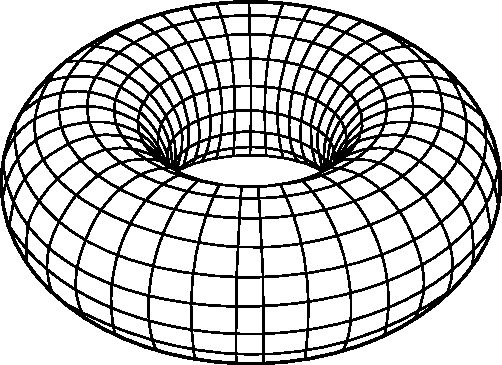
\includegraphics[width=0.8\textwidth]{torus2.pdf}
	\end{center}
\end{titlepage}
%\maketitle
\setcounter{tocdepth}{1}
\tableofcontents

\section*{Zusammenfassung}
Dies ist ein Mitschrieb der Vorlesung “Einführung in die Geometrie und Topologie” vom Wintersemester 2011/2012 am Karlsruher Institut für Technologie, die von Herrn Prof. Dr. Wilderich Tuschmann gehalten wird.

\setcounter{chapter}{-1}
\chapter{Einführung}
\setcounter{section}{-1}

Topologie ist qualitative Geometrie. Ihr grundlegendes Studienobjekt sind topologische Räume und Abbildungen zwischen diesen.

\begin{definition}{Topologischer Raum}
Ein \underline{topologischer Raum} $X$ ist gegeben durch eine Menge $X$ und ein System $\OO$ von Teilmengen von $X$, den so genannten \underline{offenen Mengen} von $X$, welches unter beliebigen Vereinigungen und endlichen Durchschnitten abgeschlossen ist und $X$ und die leere Menge $\emptyset$ als Elemente enthält.
\newline
$X$ Menge, $\OO \subset \mathcal{P}(X) \colon$
\begin{enumerate}[(1)]
	\item $O_1, O_2 \in \OO \Rightarrow O_1 \cap O_2 \in \OO$
	\item $O_\alpha \in \OO, \alpha \in A, A \text{ Indexmenge} \Rightarrow \bigcup\limits_{\alpha \in A}{O_\alpha} \in \OO$
	\item $X, \emptyset \in \OO$
\end{enumerate}
\end{definition}

\begin{bsp}{}
\OO = $\{X, \emptyset\} \Rightarrow (X,\OO)$ ist topologischer Raum!
\end{bsp}

\begin{bsp}{}
$$X \text{ Menge, }\OO = \left\{\{x\} \mid x\in X\right\} + \text{Axiome, die zu erfüllen sind} \leadsto \tilde{\OO} = \mathcal{P}(X)$$
$\Rightarrow (X,\tilde{\OO})$ ist topologischer Raum.
$\OO$ ist "Basis" der Topologie $\tilde{\OO}$.
\end{bsp}

\begin{definition}{Metrischer Raum}
Ein \underline{metrischer Raum} $X$ ist eine Menge $X$ mit einer Abbildung $d \colon X \times X \rightarrow \R$, der \underline{"Metrik"} auf $X$, die folgende Eigenschaften erfüllt:
$\forall x,y,z \in X$ gilt:
\begin{enumerate}[(1)]
	\item $d(x,y) = d(y,x)$ \underline{"Symmetrie"}
	\item $d(x,y) = 0 \Leftrightarrow x = y, d(x,y) \geq 0$ \underline{"Definitheit"}
	\item $d(x,z) \leq d(x,y) + d(y,z)$ \underline{"Dreiecksungleichung"}
\end{enumerate}
\end{definition}

\begin{definition}{Stetigkeit}
Eine Abbildung $F \colon X \rightarrow Y$ zwischen topologischen Räumen $X$ und $Y$ heißt \underline{stetig}, falls die F-Urbilder offener Mengen in $Y$ offene Teilmengen von $X$ sind.
\end{definition}

\begin{figure}[h]
\centering
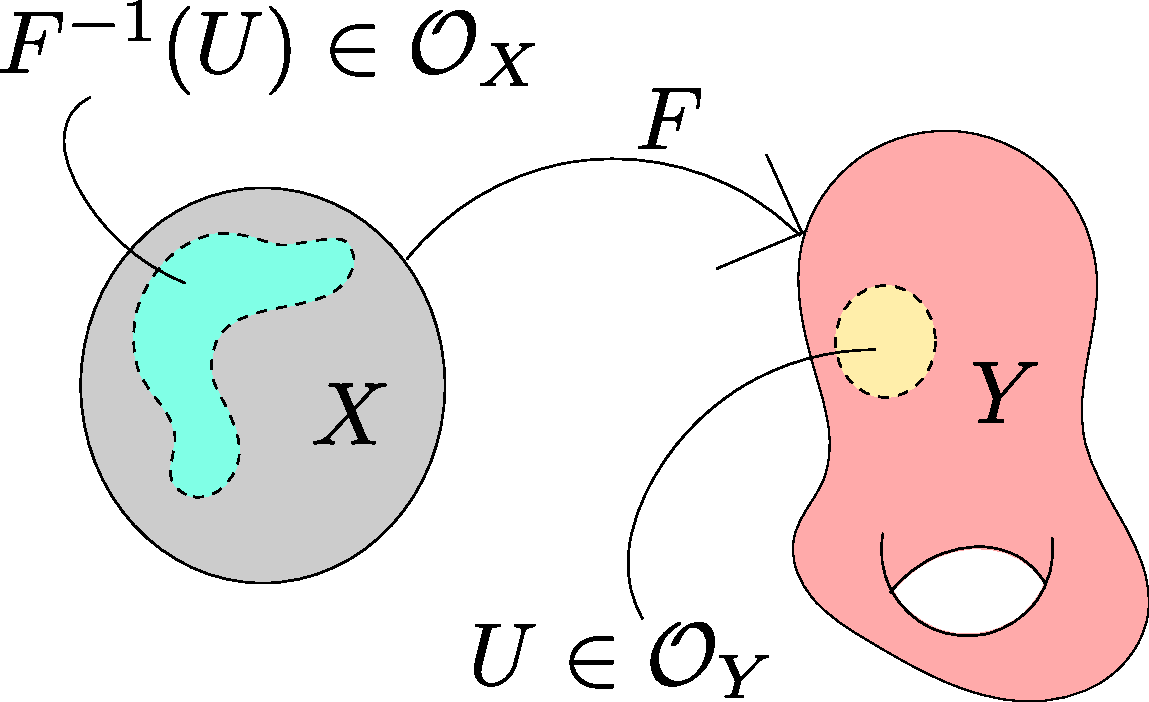
\includegraphics[width=0.3\textwidth]{images/stetigeAbb.pdf}
\caption{Stetige Abbildung}
\end{figure}

\begin{remark}
Ist $(X,d)$ ein metrischer Raum, so sind die offenen Mengen der von der Metrik induzierten Topologie\footnote{siehe später} Vereinigungen von endlichen Durchschnitten von Umgebungen
$U_{\epsilon}(x):=\{y \in X \mid d (x,y) < \epsilon \} (\epsilon > 0)$, 
und $F \colon (X,d) \rightarrow (Y,d')$ ist stetig im obigen Sinn genau dann, falls für alle $\epsilon > 0$ und alle $x \in X$ ein $\delta > 0$ existiert mit $F(U_\delta (x)) \subset U_\epsilon (F(x))$.
\end{remark}

\begin{definition}{Homotopie}
Eine \underline{Homotopie} $H \colon f \simeq g$ zwischen zwei (stetigen) Abbildungen $f,g \colon X \rightarrow Y$ ist eine (stetige) Abbildung $$H \colon X \times I \rightarrow Y, (x,t) \mapsto H(x,t)$$ 
mit $H(x,0) = f(x) \text{ und } H(x,1) = g(x) \quad \forall x \in X$.
\newline
(Hier ist $I = [0,1] \subset \R$)
\newline
$f$ und $g$ heißen dann \underline{homotop}, in Zeichen: $f \simeq g$.
\end{definition}

\paragraph{Achtung:} "Stetig" meint hier im Sinne der Produkt-Topologie (siehe später) auf $
X \times I$.

\begin{figure}[h]
\centering
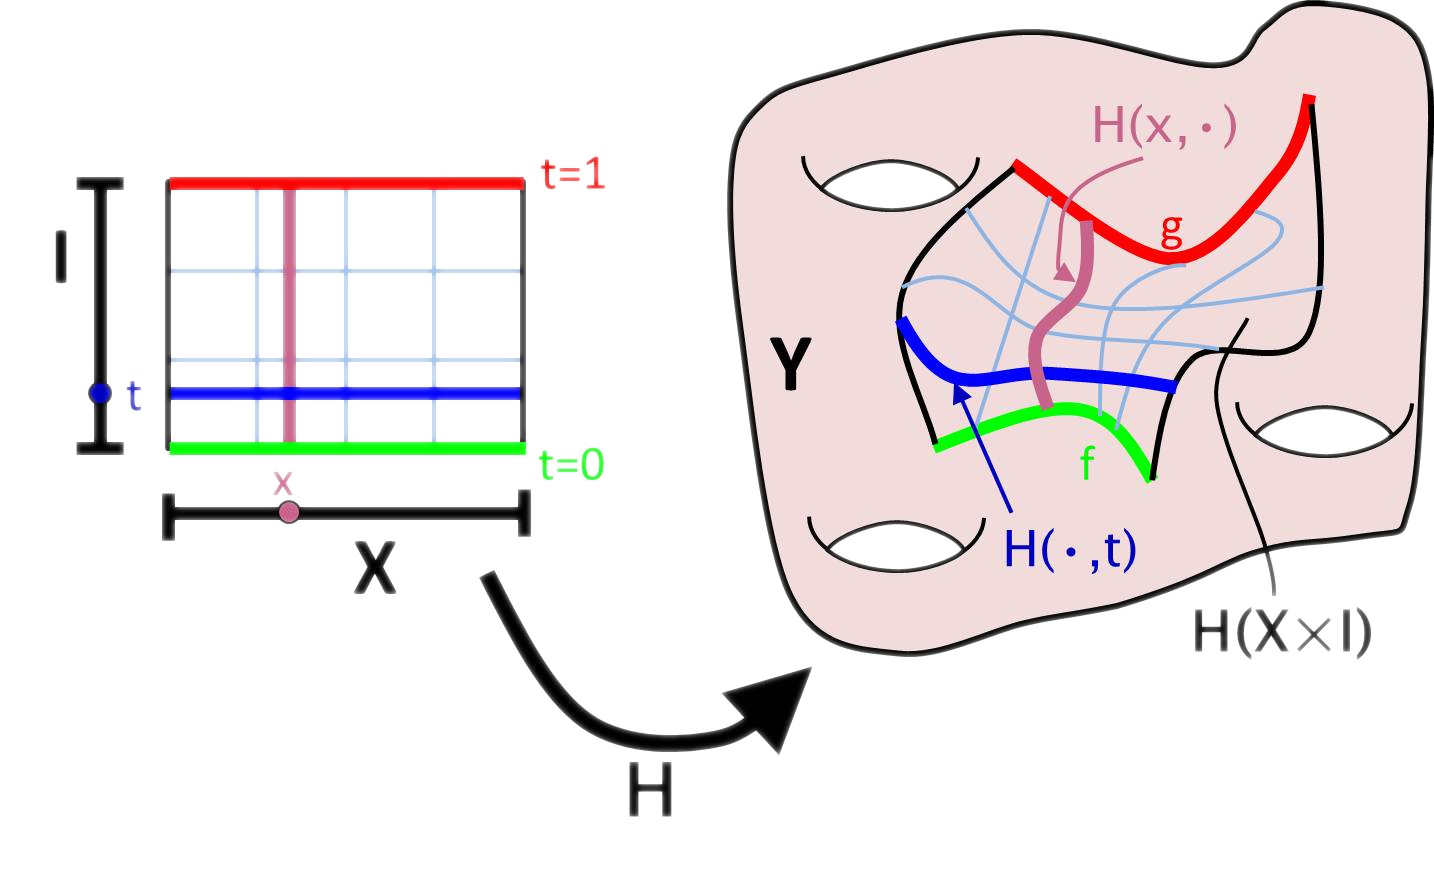
\includegraphics[width=0.5\textwidth]{images/Homotopie.png}
\caption{Homotopie}
\end{figure}

\begin{figure}[h]
\centering
\subfloat{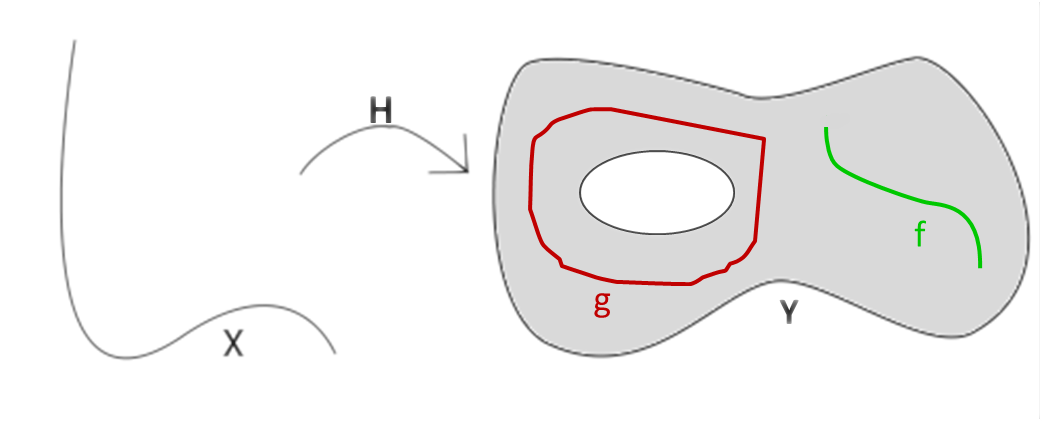
\includegraphics[width=0.5\textwidth]{images/nicht_homotop_1.png}}\qquad
\subfloat{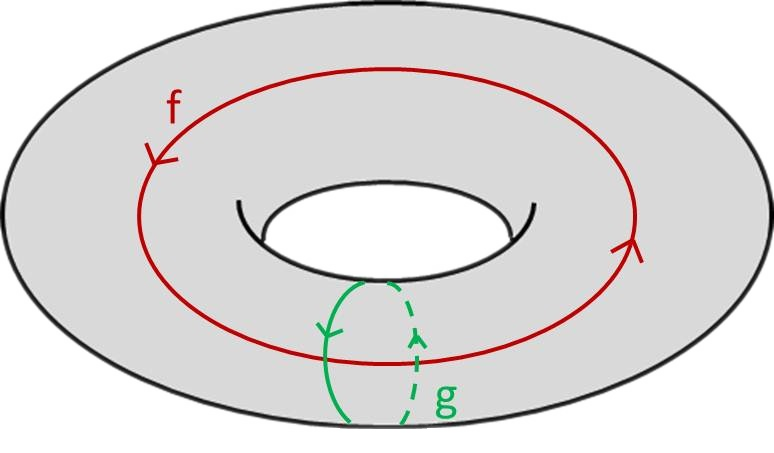
\includegraphics[width=0.4\textwidth]{images/nicht_homotop_2.png}}
\caption{f und g sind jeweils homotop, vgl. Bemerkung \ref{nichttrivial}!}
\end{figure}

\begin{remark}
$H$ heißt auch \underline{Homotopie} \underline{\underline{von $f$ nach $g$}}. Eine solche ist auch interpretierbar als eine stetige parametrisierte Schar.
\end{remark}

\begin{figure}[h]
\centering
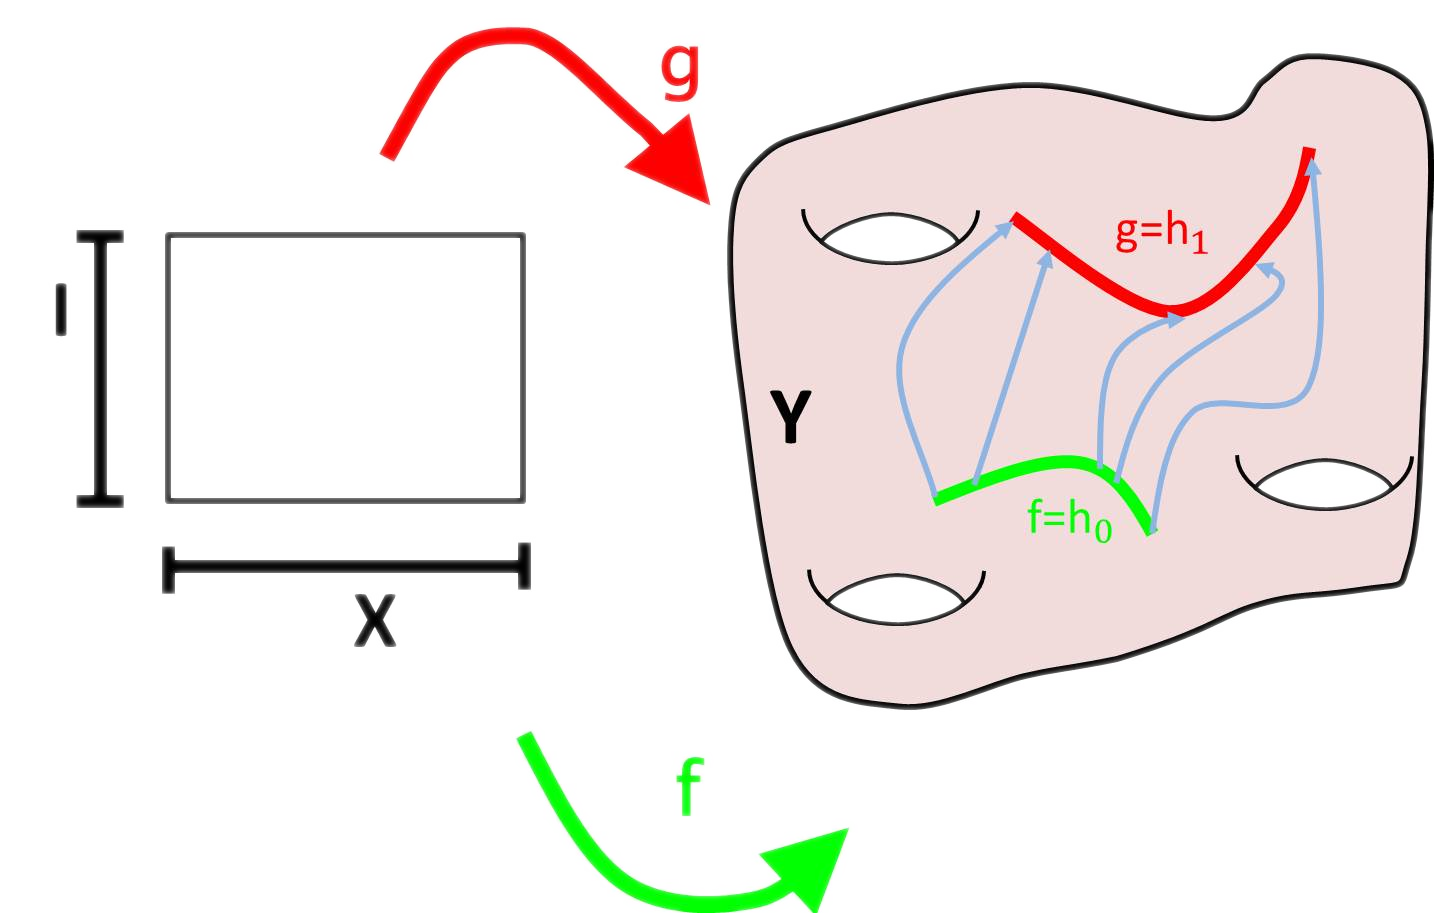
\includegraphics[width=0.5\textwidth]{images/Homotopie_param.png}
\caption{$H = (h_t), t \in [0,1]$, von stetigen Abbildungen $h_t \colon X \rightarrow Y$ mit \underline{Anfang} $h_0=f$ und \underline{Ende} $h_1=g$.}
\end{figure}


\begin{definition}{Homotope Abbildungen $f,g \colon X \rightarrow Y$}
	Zwei (stetige) Abbildungen heißen \underline{homotop}, in Zeichen: $f \simeq g$, falls eine Homotopie mit Anfang $f$ und Ende $g$ existiert.
\end{definition}

\begin{remark}
"Homotop sein" ist eine Äquivalenzrelation.
\end{remark}

\begin{proof}
	\underline{Symmetrie}:
	Gilt für $f,g \in C(X,Y) := \{F \colon X \rightarrow Y \text{ stetig } \}$ $f \simeq g$ vermöge $H=(h_t), t \in [0,1],$ so liefert $(\tilde{h_t})$ mit $\tilde{h_t}:=h_{1-t}$ eine Homotopie von $g$ nach $f$, d.h. $f \simeq g \Leftrightarrow g \simeq f$.
	\newline
	\underline{Reflexivität}:
	$f \simeq f$ vermöge $h_t : \equiv f \forall t \in [0,1]$
	\newline
	\underline{Transitivität}:
	Es sei $f \simeq g$ vermöge $(h_t)$ und ferner $g \simeq l$ vermöge $(k_t)$.
	Dann liefert $M \colon X \times [0,1] \rightarrow Y$ mit
	$$M_t := \begin{cases} h_{2t} & 0 \leq t \leq \frac{1}{2} \\
	k_{2t-1} & \frac{1}{2} \leq t \leq 1
	\end{cases}$$
	eine Homotopie von $f$ nach $l$, d.h. $f \simeq g, g \simeq l \Rightarrow f \simeq l$.
\end{proof}

\begin{figure}[h]
\centering
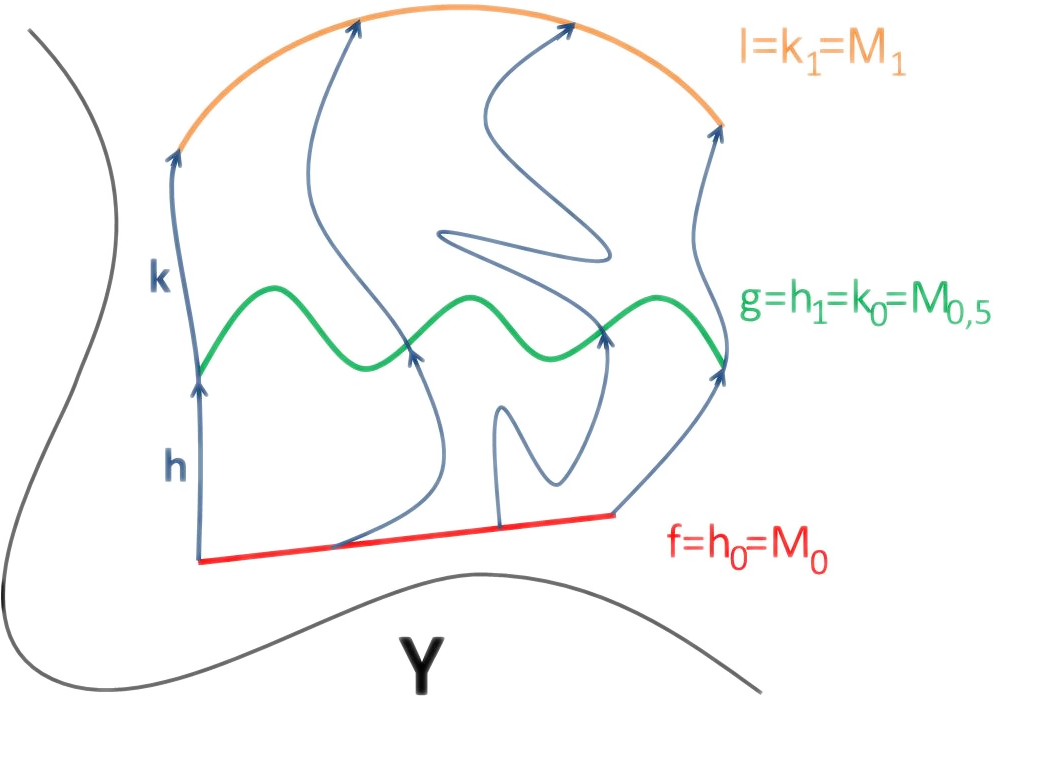
\includegraphics[width=0.5\textwidth]{images/Homotopie_Transitivitaet.png}
\caption{Transitivität der Relation "homotop sein"}
\end{figure}

\begin{remark}
Die Äquivalenzrelation "Homotopie von Abbildungen" liefert also eine Partition von $C(X,Y)$ in Äquivalenzklassen. Diese heißen Homotopieklassen und die \underline{Menge aller Homotopieklassen} \underline{stetiger Abbildungen} \underline{von $X$ nach $Y$} wird mit $[X,Y]$ bezeichnet.
\begin{figure}[h]
\centering
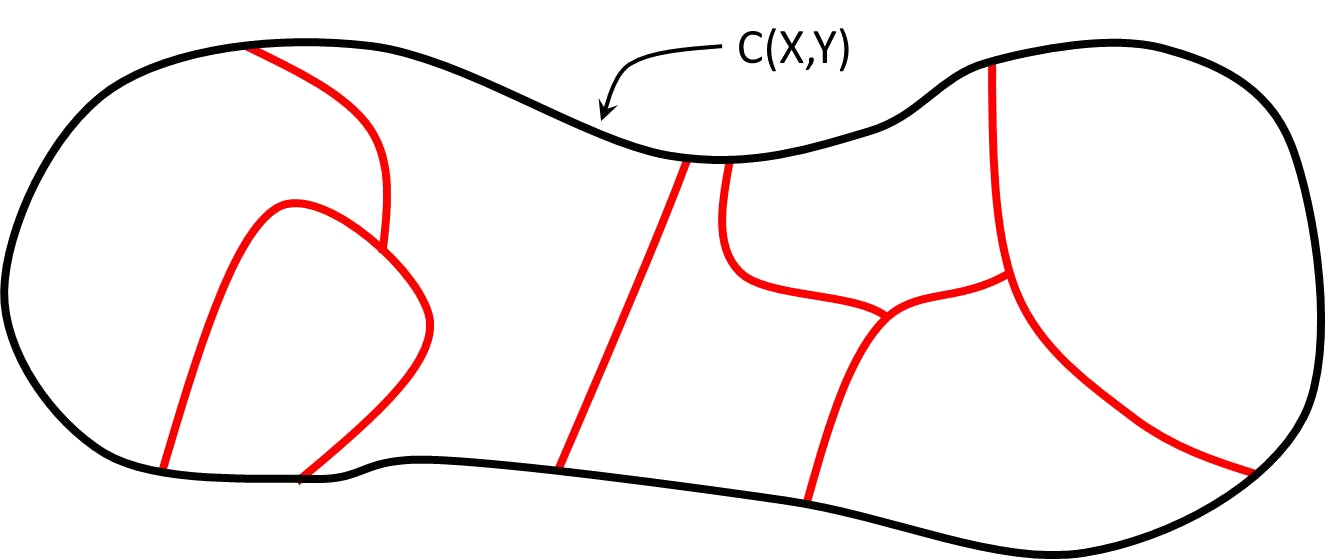
\includegraphics[width=0.5\textwidth]{images/Aequivalenzklassen.png}
\caption{Äquivalenzklassen $[X,Y]$ von $C(X,Y)$}
\end{figure}
\end{remark}

\begin{remark}
$C(X,Y)$ ist im Allgemeinen \underline{\underline{viel}} schwieriger zu verstehen als $[X,Y]$!
\end{remark}

\begin{bsp}{}
Je zwei stetige Abbildungen $f,g \colon X \rightarrow \R^n$ sind homotop! Denn 
$$H(x,t):= (1-t) f(x) + t \cdot g(x)$$ liefert eine Homotopie von $f$ nach $g$:
\begin{figure}[h]
\centering
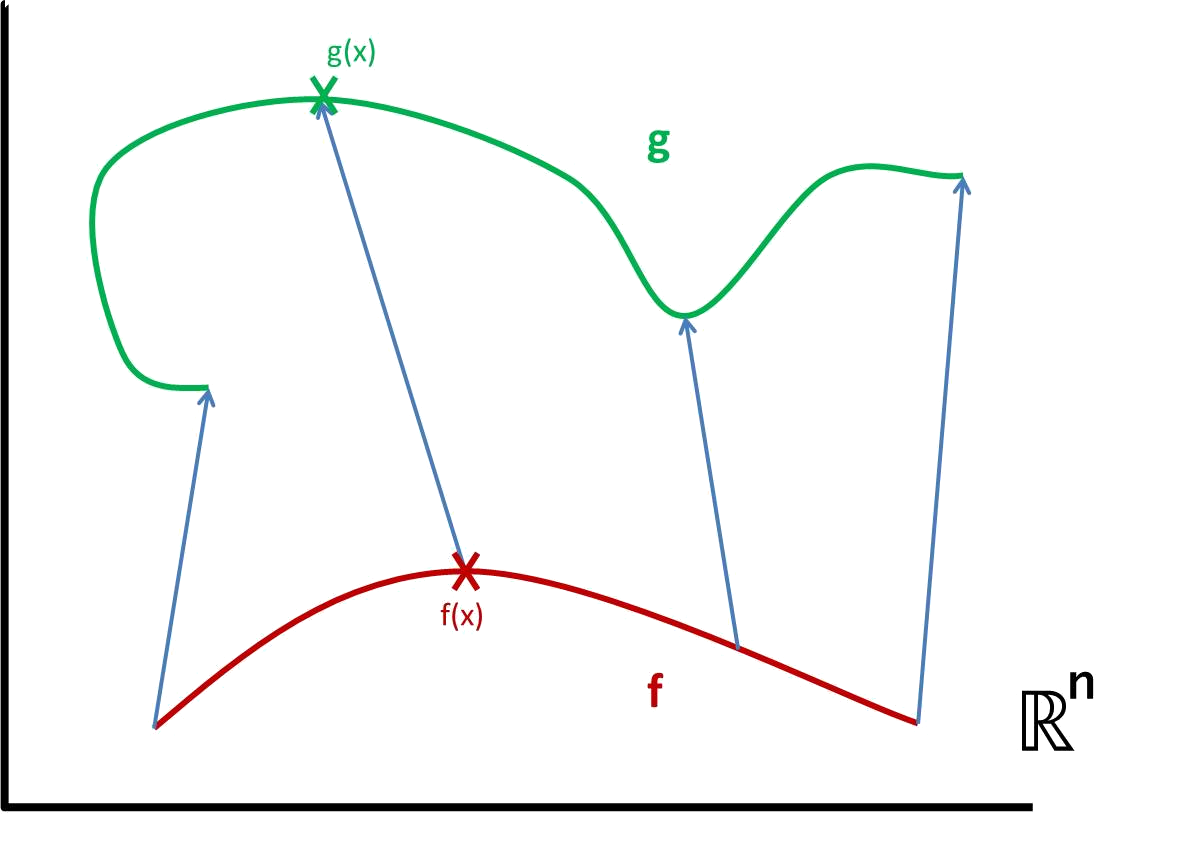
\includegraphics[width=0.5\textwidth]{images/R_n_immer_homotop.png}
\caption{Zwei stetige Abbildungen $f,g \colon X \rightarrow \R^n$ sind immer homotop.}
\end{figure} 
\end{bsp}

\begin{definition}{Nullhomotopie}
Eine stetige Abbildung $f \colon X \rightarrow Y$ heißt \underline{nullhomotop}, falls sie homotop zu einer konstanten Abbildung ist.
\end{definition}

\begin{figure}[h]
\centering
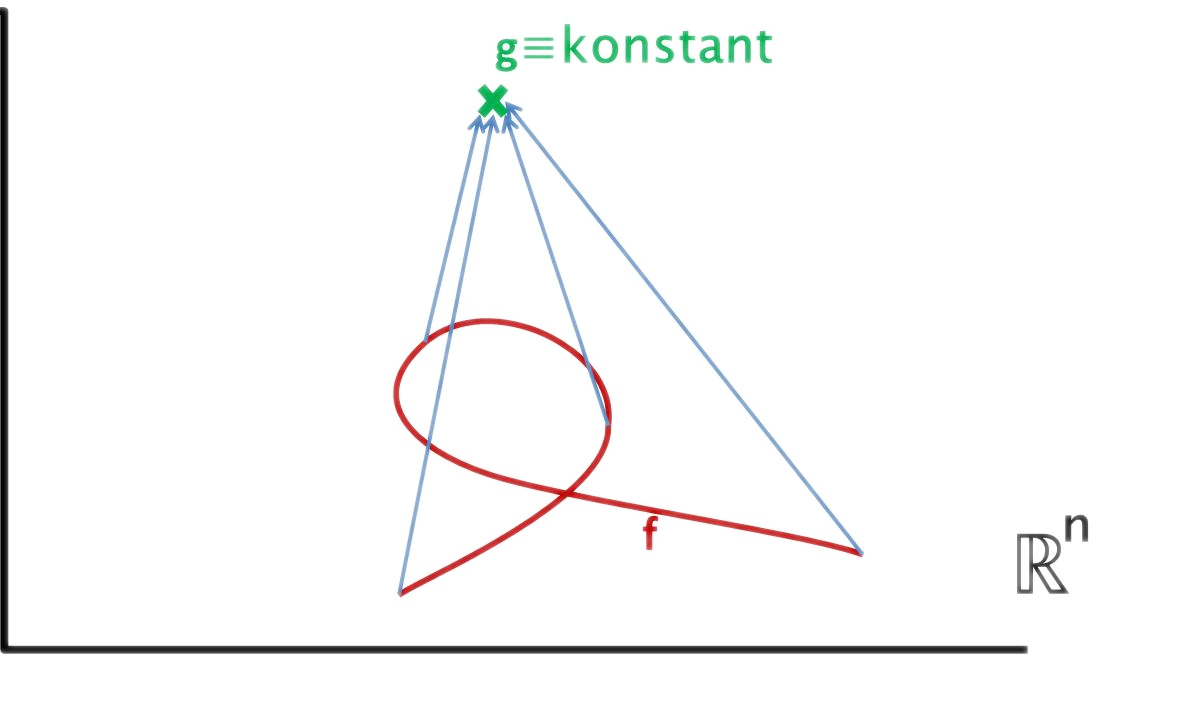
\includegraphics[width=0.5\textwidth]{images/Nullhomotopie.png}
\caption{f ist nullhomotop.}
\end{figure}

\begin{corollary}
Jede stetige Abbildung $f \colon X \rightarrow \R^n$ ist nullhomotop, d.h. für jeden topologischen Raum $X$ besteht $[X, \R^n]$, $n$ beliebig, nur aus einem Punkt!
\end{corollary}

\begin{bsp}{}
Jeder \underline{geschlossene Weg im $\R^2$}, d.h. jede stetige Abbildung $f \colon [0,1] \rightarrow \R^2$ mit $f(0) = f(1)$ ist nullhomotop.
$\bigl[[0,1], \R^2\bigr]$ + gleicher Anfangs- und Endpunkt besteht nur aus einem Punkt, zum Beispiel der Äquivalenzklasse der konstanten Kurve $t \mapsto (1,0)$.

\begin{figure}[h]
\centering
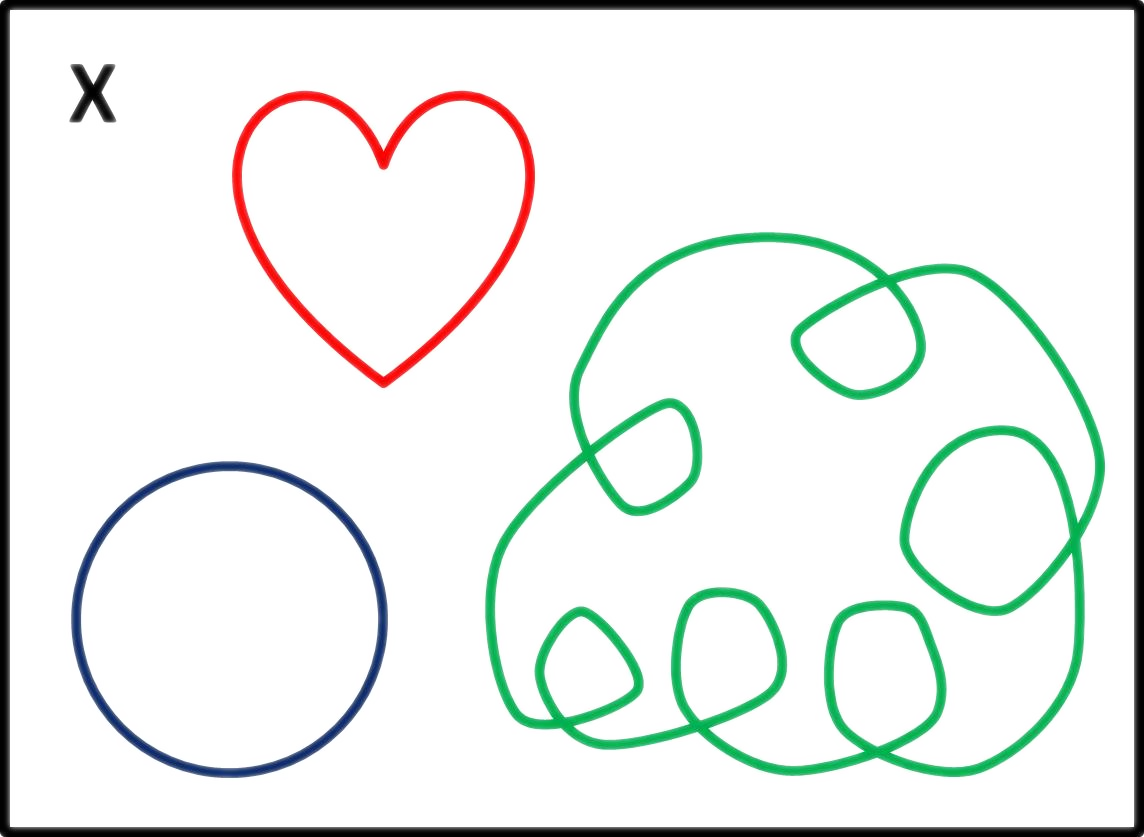
\includegraphics[width=0.5\textwidth]{images/Geschlossene_Wege.png}
\caption{Geschlossene Wege in $\R^n$.}
\end{figure}

\begin{remark}{}\label{nichttrivial}
Interpretiere einen geschlossenen Weg im $\R^2$ auch als stetige Abbildung von $S^1 := \{ x \in \R^2 \mid \text{ } ||x|| = 1\}$ in $\R^2$, so gilt also $[S^1, \R^2]$ ist einelementig.
\newline
\underline{Aber} $[S^1, \R^2 \backslash \{0\}]$ ist nichttrivial, wenn für $f \colon S^1 \rightarrow \R^2 \backslash \{0\}$ der Punkt $f(1), 1 = (1,0) \in S^1$, unter allen betrachteten Homotopien festgelassen werden soll. Dieses Phänomen wird uns zum Studium der Fundamentalgruppe führen \ldots
\end{remark}

\begin{figure}[h]
\centering
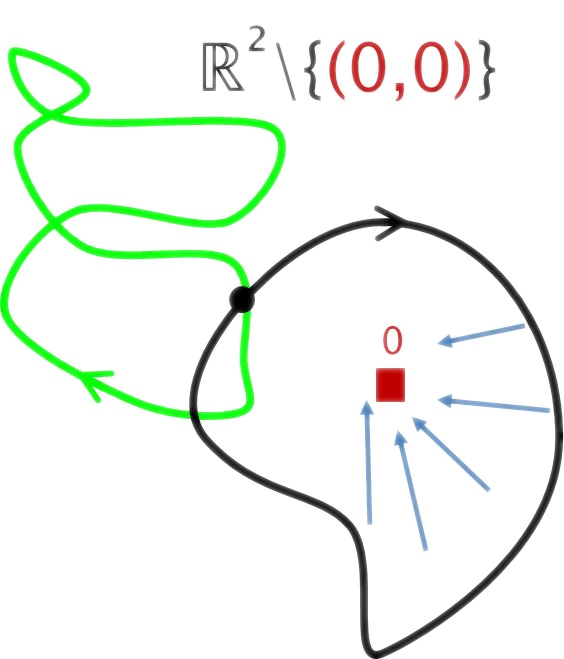
\includegraphics[scale=0.4]{images/Homotop_Schleifen_R_ohne_0.png}
\caption{$[S^1, \R^2 \backslash \{0\}]$ ist nichttrivial.}
\end{figure}
\end{bsp}

\begin{figure}[h]
\centering
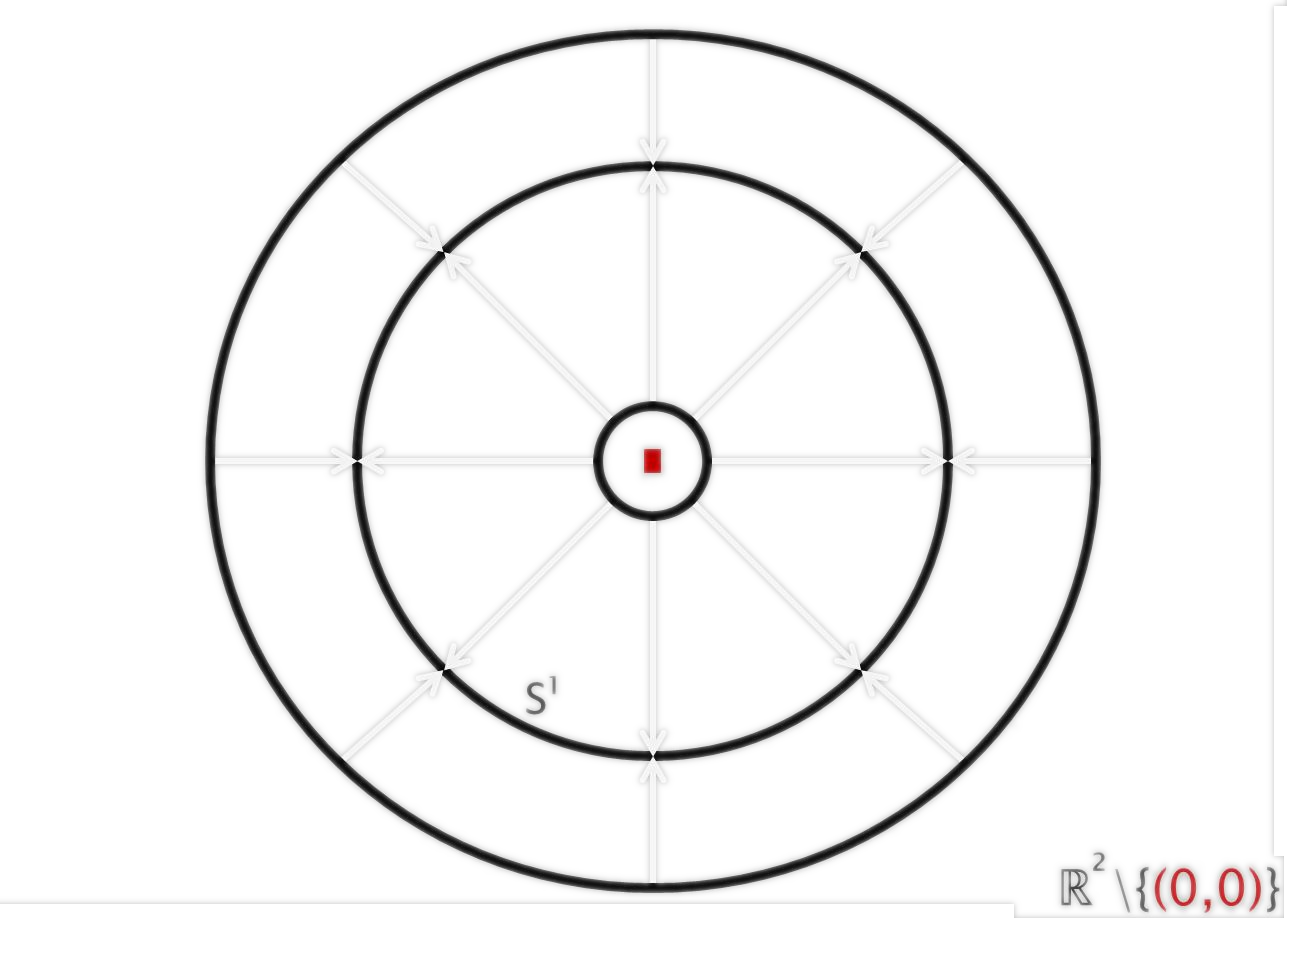
\includegraphics[width=0.5\textwidth]{images/S1_und_R2_ohne_0.png}
\caption{$[S^1,\R^2\backslash\{(0,0)\}]\text{ "=" }[S^1,S^1]$.}
\end{figure}



\newpage
\renewcommand{\thechapter}{\Roman{chapter}}
\chapter{Grundlagen der Allgemeinen Topologie}
\section{Erste Beispiele topologischer Räume}
\begin{bsp}{}
	\begin{enumerate}[(1)]
		\item $X, \OO := \{X, \emptyset\}$ \underline{`triviale Topologie'}
		\item $X, \OO := \mathcal{P}(X)$ \underline{`diskrete Topologie'}
		\item Metrische Räume, siehe unten
		\item $X:= \{a,b,c,d\} \Rightarrow \OO := \left\{X, \emptyset, \{a\}, \{b\}, \{a,c\}, \{a,b,c\}, \{a,b\} \right \}$ definiert eine Topologie auf $X$, aber $\OO^\prime:= \left \{ X, \emptyset, \{a,c,d\}, \{b,d\} \right \}$ nicht!
		\item $X := \R, \OO := \{O \mid \text{O ist Vereinigung von Intervallen } (a,b) \text{ mit } a,b \in \R\}$. $\Rightarrow (X, \OO) \text{ ist topologischer Raum}$, und $\OO$ heißt \underline{Standard-Topologie}.
		\item $X:= \R, \tilde{\OO} := \{O \mid O = \R \backslash E, E \subset \R \text{ endlich}\} \cup \{\emptyset\}$ ist auch eine Topologie auf $\R$, die so genannte $\mathcal{T}_1$-Topologie.
	\end{enumerate}
\end{bsp}

\begin{definition}{Teilraumtopologie}
Es sei $(X, \OO)$ topologischer Raum und $A \subset X$. Die auf $A$ durch
$$\OO \Big |_{A} := \{U \cap A \mid U \in \OO \}$$
induzierte Topologie heißt \underline{Teilraumtopologie} und der dadurch gegebene topologische Raum $(A, \OO \Big |_{A})$ heißt \underline{Teilraum} von $(X, \OO)$.
\end{definition}

\begin{remark}
$B \subset A$ ist also genau dann \underline{offen \underline{in $A$}}, wenn $B$ der Schnitt einer \underline{in $X$} offenen Menge mit $A$ ist.
\end{remark}

\begin{bsp}{}
$X = \R^2, A = S^1 = \{ x \in \R^2 \mid \text{ } ||x|| = 1\}$ 
\newline
\begin{figure}[h]
\centering
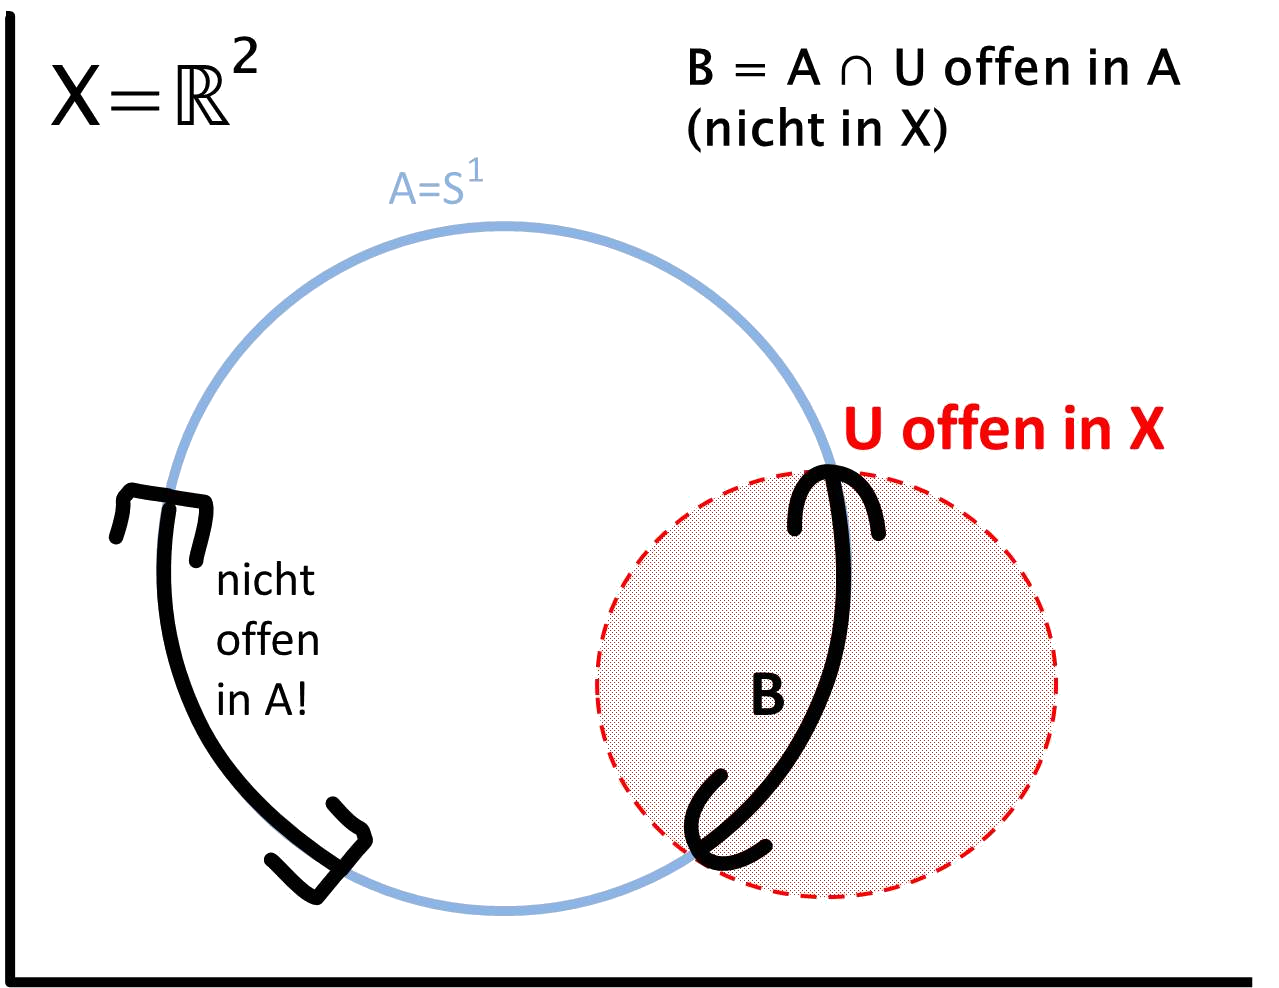
\includegraphics[width=0.5\textwidth]{images/Teilraumtopologie.png}
\end{figure}
\newline
\underline{Achtung:} $B$ ist \underline{\underline{nicht}} offen in $\R^2$!
\end{bsp}

\section{Topologische Grundbegriffe}

\begin{definition}{Abgeschlossenheit}
	$A \subset X, X$ topologischer Raum, heißt \underline{abgeschlossen} $$:\Leftrightarrow X \backslash A \text{ ist offen.}$$
\end{definition}

Die De Morgan'schen Regeln der Mengenlehre zeigen:

\begin{remark}
	Beliebige Durchschnitte abgeschlossener Mengen sind abgeschlossen, ebenso endliche Vereinigungen und genauso $X$ und $\emptyset$.
\end{remark}

\begin{bsp}{}
	In einem diskreten topologischen Raum sind \underline{alle Teilmengen} abgeschlossen, in $\R_{\mathcal{T}_1}$\footnote{$\R$ mit $\mathcal{T}_1$-Topologie} alle endlichen Teilmengen und $X, \emptyset$.
\end{bsp}

\begin{definition}{Umgebung}
	Ist $X$ topologischer Raum und $x \in X$, so heißt jede \underline{offene} Teilmenge $O \subset X$ mit $x \in O$ eine \underline{Umgebung} von $x$.
\end{definition}

\begin{remark}
	Umgebungen sind per definitionem offen! \newline
	\begin{figure}[h]
		\centering
		\subfloat{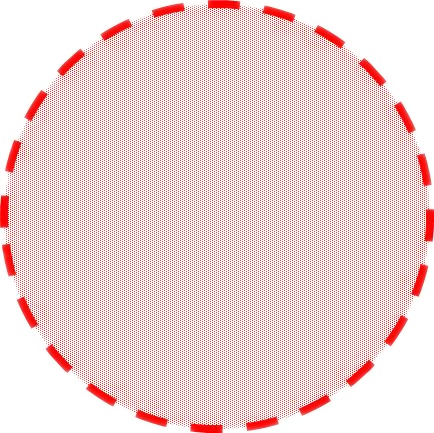
\includegraphics[scale=0.3]{images/offener_Kreis.png}} $\qquad\qquad$ 				\subfloat{
\includegraphics[scale=0.3]{images/offenes_Quadrat.png}} 
	\end{figure}
\end{remark}

\begin{remark}
	Jede offene Teilmenge von $\R_{Standard}$ ist eine Vereinigung disjunkter offener Intervalle, doch abgeschlossene Teilmengen von $\R$ sind keinesfalls immer Vereinigungen abgeschlossener Intervalle!
\end{remark}

\begin{bsp}{Die \underline{Cantor-Menge} $\mathcal{C}:= \left \{ x \in \R \mid x = \sum\limits_{k=1}^{\infty}{\frac{a_k}{3^k}}, a_k \in \{0,2\} \right \}$}
	$\Rightarrow$ $\mathcal{C}$ ist abgeschlossen in $\R$, enthält überabzählbar viele Elemente und hat `Hausdorff-Dimension' $\frac{\ln 2}{\ln 3} \approx 0,6 \ldots$
\end{bsp}

\begin{figure}[h]
\centering
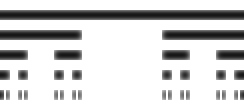
\includegraphics[width=0.5\textwidth]{images/Cantormenge_5te_Iteration.png}
\caption{Die Cantor-Menge.}
\end{figure}

\begin{definition}{Basis}
	Ist $(X, \OO)$ topologischer Raum mit $\mathcal{B} \subset \OO$, 
	\newline
	so heißt $\mathcal{B}$ \underline{Basis der Topologie} $:\Leftrightarrow$ Jede (nichtleere) offene Menge ist Vereinigung von Mengen aus $\mathcal{B}$.
\end{definition}

\begin{bsp}{}
	\begin{enumerate}[(1)]
		\item Die offenen Intervalle bilden eine Basis der Standard-Topologie von $\R$.
		\item Sämtliche offenen\footnote{bezüglich der euklidischen Metrik} Kreisscheiben 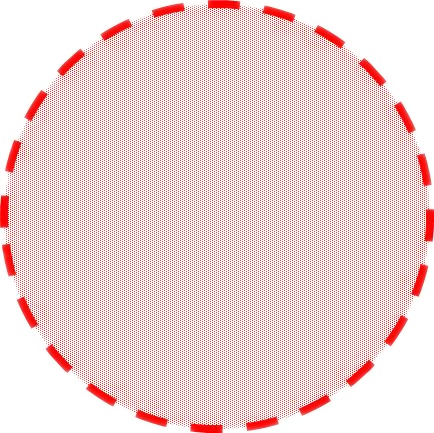
\includegraphics[scale=0.07]{images/offener_Kreis.png} und auch sämtliche offenen Quadrate 
\includegraphics[scale=0.07]{images/offenes_Quadrat.png} bilden Basen ein und derselben Topologie auf $\R^2$.
	\end{enumerate}
\end{bsp}

\begin{remark}
	$\bullet$ $\mathcal{B} \subset \OO$ ist Basis der Topologie von $X$ $\Leftrightarrow \forall O \in \OO \forall x \in O \exists B \in \mathcal{B} \colon x \in B \subset O$.
	\newline
	$\bullet$ $\mathcal{B} \subset \mathcal{P}(X)$ bildet die Bais \underline{einer} Topologie auf $X$ $\Leftrightarrow$ $X$ ist Vereinigung von Mengen aus $\mathcal{B}$ und der Schnitt je zweier Mengen aus $\mathcal{B}$ ist eine Vereinigung von Mengen aus $\mathcal{B}$.
	\newline
	\begin{figure}[h]
		\centering
		\subfloat{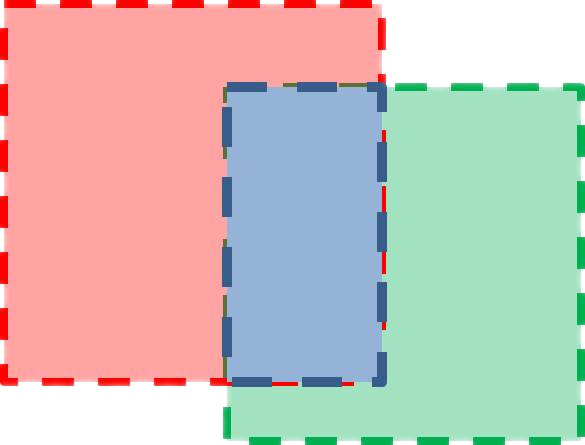
\includegraphics[scale=0.3]{images/Quadrate_Schnitt.png}}\qquad
		\subfloat{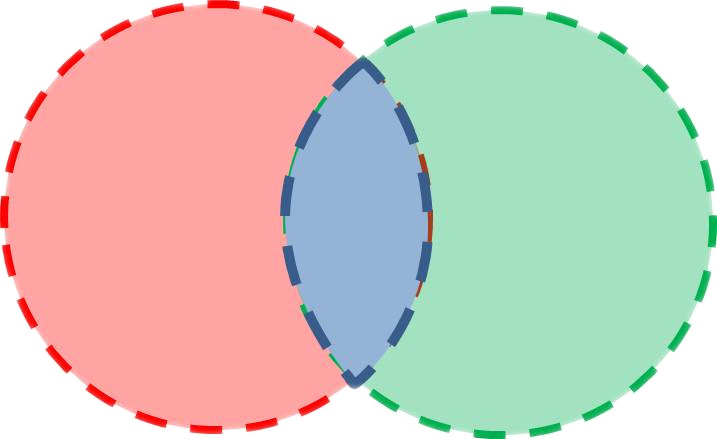
\includegraphics[scale=0.3]{images/Kreis_Schnitt.png}}
	\end{figure}
\end{remark}

\begin{definition}{Produkt-Topologie}
	Sind $(X, \OO_X)$ und $(Y, \OO_Y)$ topologische Räume, so bildet $$\mathcal{B}_{X \times Y} := \{U \times V \mid U \in \OO_X, V \in \OO_Y\}$$
	die Basis einer Topologie für die Menge $X \times Y$, und diese heißt \underline{Produkt-Topologie auf $X \times Y$}.
	\newline
	Versehen mit der Produkt-Topologie ist $X \times Y$ sebst ein topologischer Raum und für gegebene $X, Y$ denkt man sich $X \times Y$ stillschweigend mit der Produkt-Topologie versehen.
\end{definition}

\begin{bsp}{}
	$\R \times \R = \R^2$ 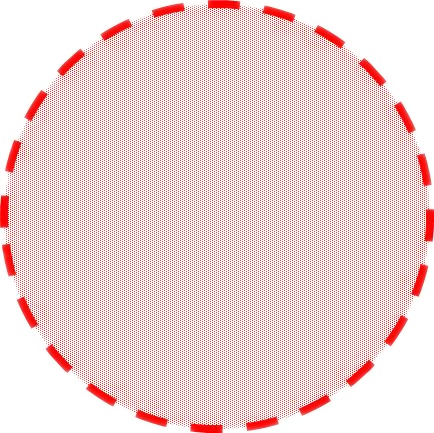
\includegraphics[scale=0.06]{images/offener_Kreis.png}
	als topologische Räume!
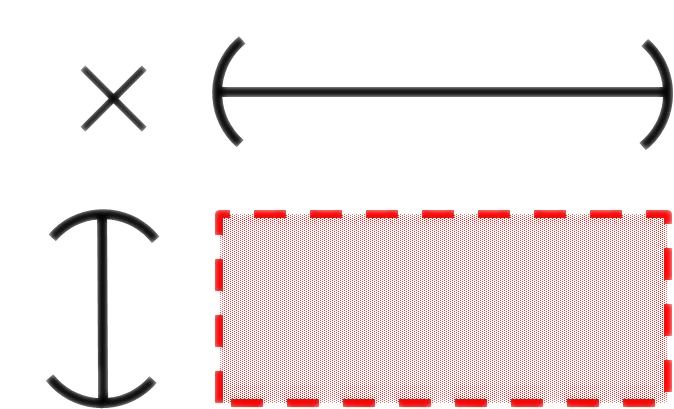
\includegraphics[scale=0.4]{images/Produkt_RxR.png} 
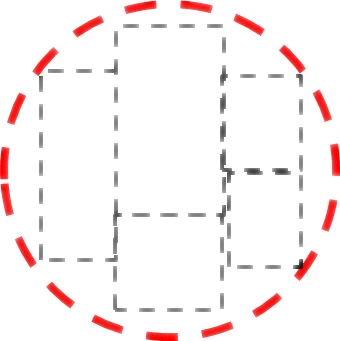
\includegraphics[scale=0.4]{images/Kreis_Rechteck.png} 
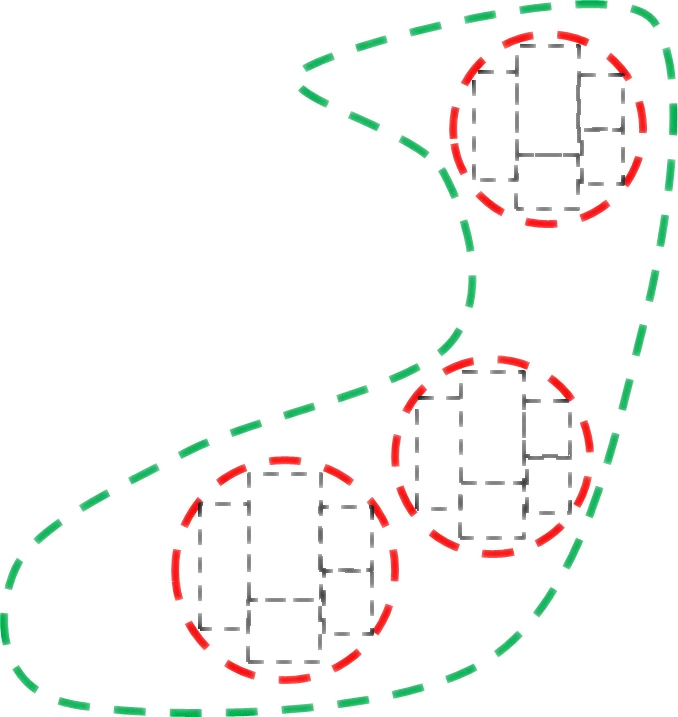
\includegraphics[scale=0.4]{images/Kreis_Rechteck_Basis.png} 
	Ebenso: $(\R^1)^n = \R^n$!
\end{bsp}

\begin{definition}{Feiner und gröber}
	Sind $\OO_1$ und $\OO_2$ Topologien auf $X$ und $\OO_1 \subset \OO_2$, 
	\newline so heißt $\OO_2$ \underline{feiner} als $\OO_1$ und $\OO_1$ \underline{gröber} als $\OO_2$.
\end{definition}

\begin{bsp}{}
	$\bullet$ Die triviale Topologie ist die gröbste Topologie auf $X$, die diskrete Topologie die feinste.
	\newline
	$\bullet$ Die Standard-Topologie auf $\R$ ist feiner als die $\mathcal{T}_1$-Topologie.
\end{bsp}

\newpage
\paragraph{Mehr zu metrischen Räumen}

\begin{definition}{$\epsilon$-Ball, Sphäre}
	Für einen metrischen Raum $(X,d)$ und $\epsilon > 0$ sei für $p \in X$
	\begin{itemize}
		\item $B_\epsilon(p):=\{x \in C \mid d(p,x) < \epsilon \}$ der \underline{offene $\epsilon$-Ball um $p$}
		\item $D_\epsilon(p):=\{x \in C \mid d(p,x) \leq \epsilon \}$ der \underline{abgeschlossene $\epsilon$-Ball um $p$}
		\item $S_\epsilon(p):=\{x \in C \mid d(p,x) = \epsilon \}$ die \underline{ $\epsilon$-Sphäre} um $p$ (oder \underline{Sphäre vom Radius $\epsilon$} um $p$)
	\end{itemize}
\end{definition}

\begin{definition}{Metrischer Unterraum}
	Ist $(X,d)$ metrischer Raum und $A \subset X$, so heißt der metrische Raum $(A, d \big |_{A \times A})$ \underline{(metrischer) Unterraum von $X$}.
\end{definition}

\begin{bsp}{}
	Für $X=\R_{Eukl.}^{n}$ sind $B_1(0), D_1(0) =: D^n$ und $S^{n-1}:=S_1(0)$ metrische Unterräume und heißen auch offener bzw. abgeschlossener Einheitsball bzw. $(n-1)$-Sphäre.
	\newline
	\begin{center}
	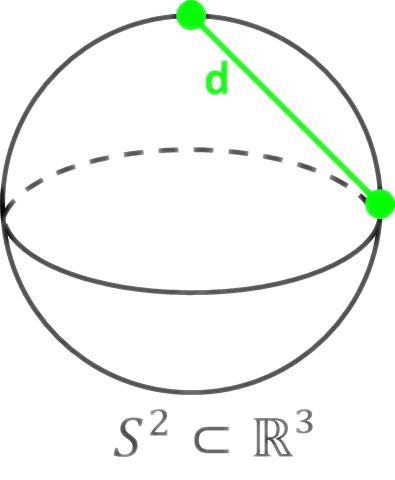
\includegraphics[width=0.3\textwidth]{images/metrischer_unterraum.png}
	\end{center}
\end{bsp}

\begin{definition}{Beschränktheit, Durchmesser}
	$A \subset (X,d)$ heißt \underline{beschränkt} \newline $:\Leftrightarrow \exists 0 < \rho \in \R \colon d(x,y) < \rho  \text{   } \forall x,y \in A$
	\newline
	Das Infimum, diam $A$, dieser $\rho$ heißt dann \underline{Durchmesser von $A$}.
	\newline
	\begin{center}
	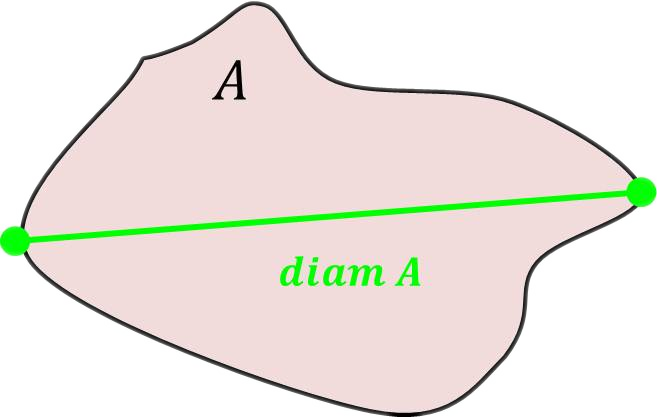
\includegraphics[width=0.4\textwidth]{images/Durchmesser.png}
	\end{center}
\end{definition}
	
\begin{remark}
	In einem metrischen Raum $(X,d)$ bilden die offenen Bälle die Basis einer Topologie $\OO=\OO_d$ von $X$, diese heißt \underline{die von der Metrik induzierte Topologie}.
\end{remark}

\begin{remark}
	$A \subset (X,d)$ ist \underline{offen}
	\newline
	$\Leftrightarrow \forall p \in A \exists \text{ ein offener Ball } B_\epsilon(p) \text{ um } p \text{ mit } B_\epsilon(p) \subset A$
	\newline
	\begin{center}
	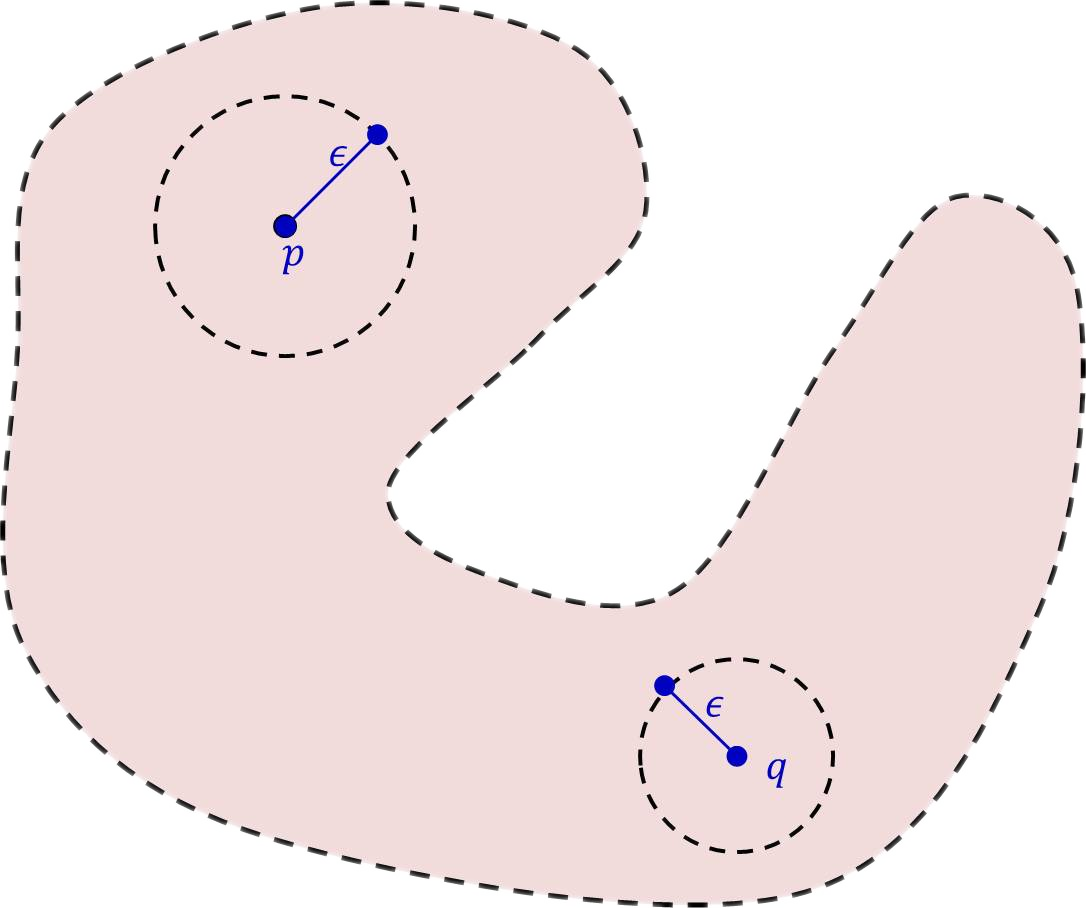
\includegraphics[width=0.5\textwidth]{images/metrisch_offen.png}
	\end{center}
\end{remark}

\begin{definition}{Abstand}
	$(X,d)$ sei metrischer Raum und $A \subset X, p \in X$.
	$$d(p,A) := dist(p,A):= \inf \{d(p,a) \mid a\in A \}$$
	heißt \underline{Abstand von $p$ und $A$}.
\end{definition}

\paragraph{Erinnerung}
Ist $(X, \OO)$ topologischer Raum und $A \subset X$, so definiert
$\OO_A := \{ A \cap O \mid O \in \OO \}$ eine Topologie auf $A$, die
 \underline{Teilraumtopologie} der \underline{in A} offenen Mengen.
 
\begin{remark}
	\label{offenAbgeschlossen}
	Ist $A \subset X$ \underline{offen} \underline{\underline{in $X$}}, so ist auch jede in $A$ offene Menge offen in $X$, und abgeschlossene\footnote{in $A$} Teilmengen einer in $X$ abgeschlossenen Menge $A$ sind auch abgeschlossen in $X$.
		
		\begin{center}
	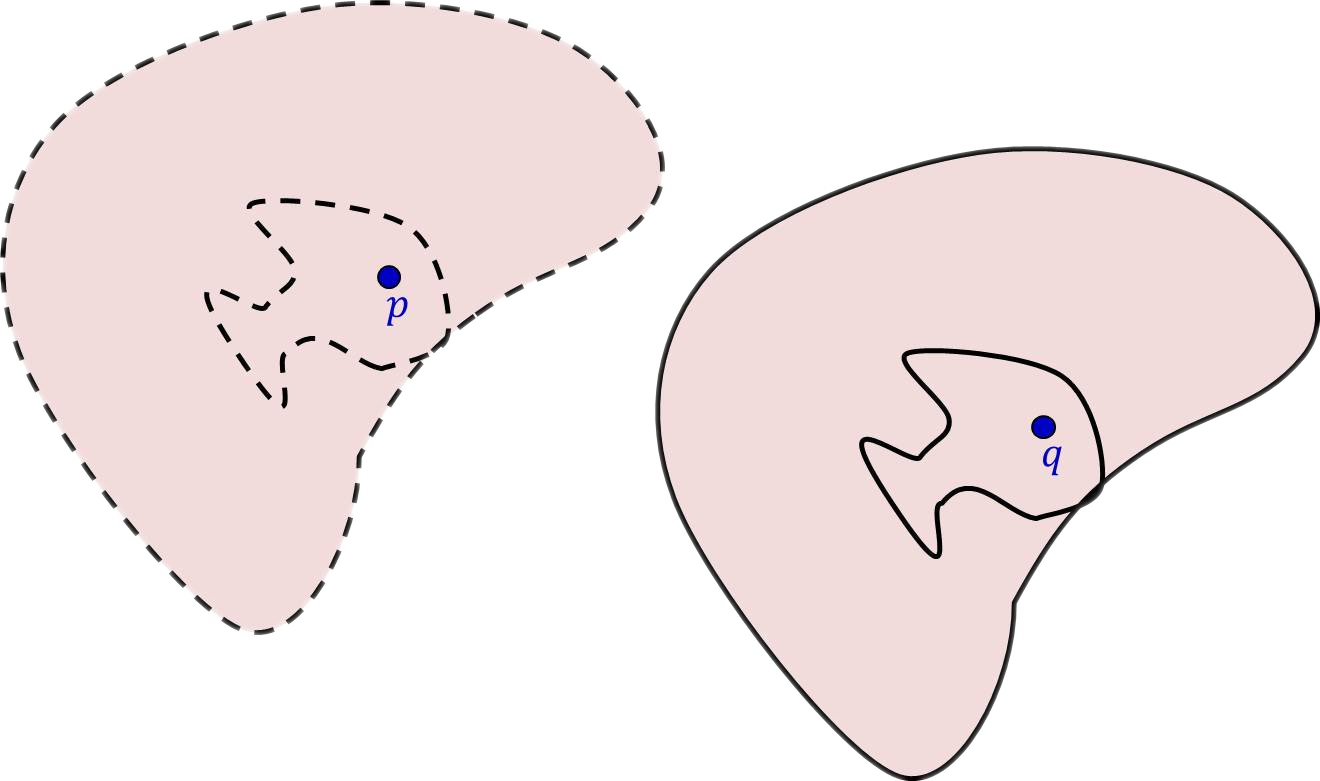
\includegraphics[width=0.5\textwidth]{images/offen_abgeschlossen.png}
	\end{center}
	Aber abgeschlossene Mengen $B$ in $A \subset X$ sind für beliebiges $A$ im Allgemeinen nicht abgeschlossen in $X$.
\end{remark}

\begin{bsp}{Beispiel zu Bemerkung~\ref{offenAbgeschlossen}}
	$B := A := (a,b) \subset X := \R$
\end{bsp}

\begin{definition}{Innerer Punkt, äußerer Punkt, Randpunkt}
	Für $p \in A \subset X$, $X$ topologischer Raum, heißt $p$
	\newline
	\begin{enumerate}[(1)]
		\item \underline{innerer Punkt} von $A$, falls es eine in $A$ enthaltene Umgebung $U$ um $p$ gibt. 
		\item \underline{äußerer Punkt}, falls eine zu $p$ disjunkte Umgebung $V$ in $X$ existiert.
		\item \underline{Randpunkt von $A$}, falls jede Umgebung von $p$ nichtleeren Durchschnitt mit $A$ und $X \backslash A$ hat.
	\end{enumerate}
\end{definition}
	\begin{center}
	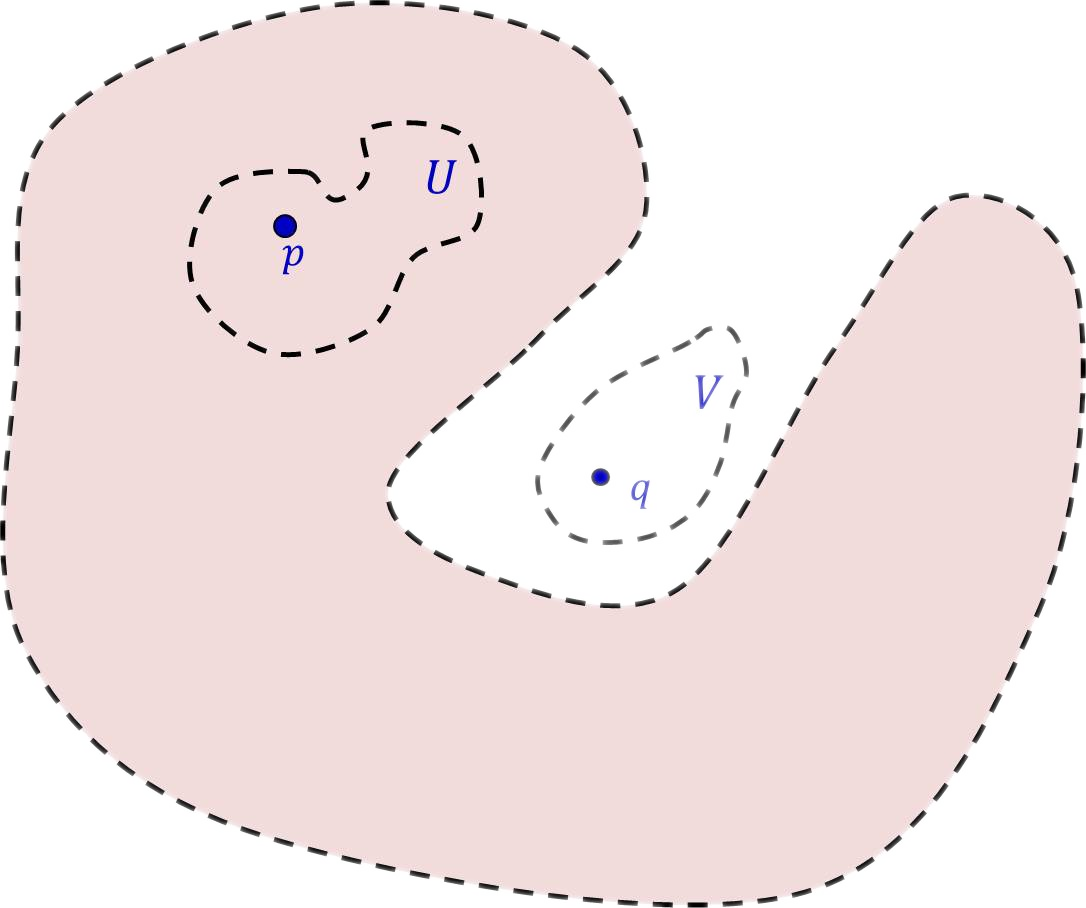
\includegraphics[width=0.5\textwidth]{images/innen_aussen.png}
	\end{center}
	
\begin{definition}{Inneres}
	Für $A \subset X$ heißt die größte in $X$ offene und in $A$ enthaltene Teilmenge $\mathring A$ \underline{Inneres von $A$}.
\end{definition}

\begin{remark}
	$\mathring A$ ist die Menge aller inneren Punkte von $A$ und die Vereinigung aller in $X$ offenen Teilmengen von $A$, und $A \text{ ist offen } \Leftrightarrow A = \mathring A$
\end{remark}

\begin{bsp}{}
	$\mathring {\R \backslash \Q} = \mathring \Q = \emptyset$
\end{bsp}

\begin{definition}{Abschluss}
	Der \underline{Abschluss} $\bar{A}$ von $A$ ist $X \backslash \left ( \mathring {(X \backslash A} ) \right )$.
\end{definition}

\begin{definition}{Rand}
	Der \underline{Rand} $\partial A$ von $A$ ist $$\partial A := \bar{A} \backslash \mathring A,$$ d.h. Rand $A$ = \{ Randpunkte von A \}.
\end{definition}

\paragraph{TODO:Exkurs zu "Randbildung (topologisch) und Ableitung (analytisch) sind dual zueinander"}

\section{Stetige Abbildungen}

\begin{definition}{Stetigkeit}
	$f \colon X \rightarrow Y$ ist stetig $:\Leftrightarrow \forall$ offenen Mengen in $Y$ ist das Urbild unter $f$ offene Menge in $X$.
\end{definition}

\begin{bsp}{}
	\begin{itemize}
		\item $f \colon X \rightarrow Y$ ist stetig $\Leftrightarrow$ Urbilder abgeschlossener Mengen sind abgeschlossen.
		\item Sind $\OO_1$ und $\OO_2$ Topologien auf $X$, so ist die Identität $\text{id} \colon (X,\OO_1) \rightarrow (X,\OO_2)$ stetig $\Leftrightarrow \OO_2 \subset \OO_1$.
		\item Für $A \subset X$ ist die Teilraumtopologie $\OO_A = \OO \big |_A$ die gröbste Topologie, bezüglich der die Inklusion $i \colon A \hookrightarrow X, a \mapsto a$ stetig ist.
	\end{itemize}
\end{bsp}

\begin{definition}{Stetigkeit}
	$f \colon X \rightarrow Y$ ist stetig in $x \in X$
	$$:\Leftrightarrow \forall \text{ Umgebungen } V \text{ von } f(x) \quad \exists \text{ Umgebung } U \text{ von } x \text{ mit }$$ $$f(U) \subset V.$$
	\newline
\end{definition}
\begin{center}
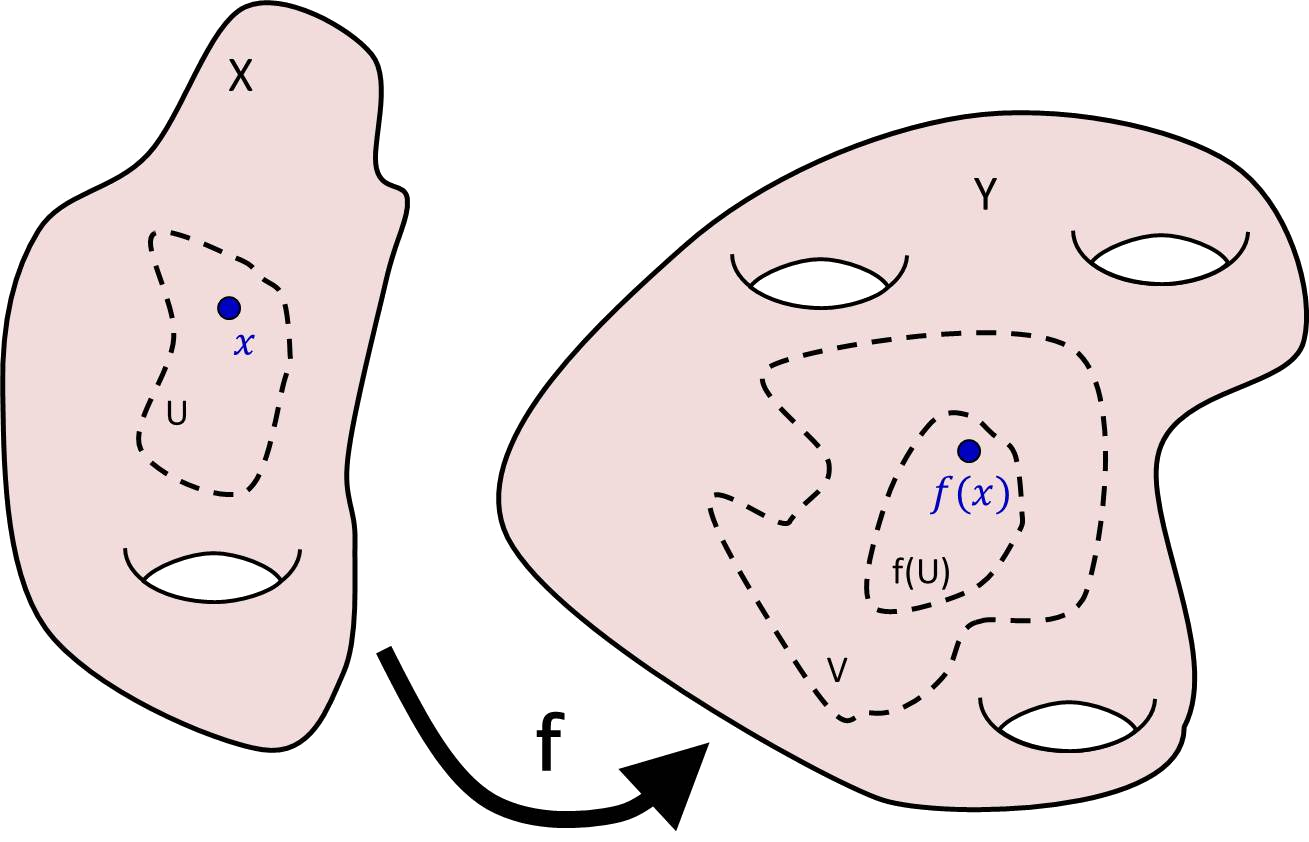
\includegraphics[width=0.5\textwidth]{images/stetig_in_x.png}
\end{center}

\begin{remark}
	$f \colon X \rightarrow Y$ ist stetig $\Leftrightarrow$ $f$ ist stetig in jedem Punkt $x \in X$.
\end{remark}

\begin{bsp}{}
	Eine Abbildung $f \colon X \rightarrow Y$ zwischen \underline{metrischen} Räumen ist bezüglich der von den Metriken induzierten Topologien stetig in $x \in X$ genau dann, wenn für jeden offenen Ball $B$ um $f(x)$ ein offener Ball um $x$ existiert, der unter $f$ in $B$ abgebildet wird. (Und ferner stetig in $x \in X$ genau dann, wenn für alle $\epsilon > 0$ ein $\delta > 0$ existiert, so dass für alle $x^\prime \in X$ mit $d_X(x,x^\prime) < \delta$ auch $d_Y \left( f(x), f(x^\prime) \right) < \epsilon$ folgt.) 
\end{bsp}

\begin{definition}{Isometrische Einbettung, Isometrie}
	Sind $X,Y$ metrische Räume, so heißt eine Abbildung $f \colon X \rightarrow Y$ \underline{isometrische Einbettung}
	\newline	
	 $: \Leftrightarrow \forall x, x^\prime \in X$ gilt $d_Y \left ( f(x), f(x^\prime) \right ) = d_X (x, x^\prime)$.
	\newline
	Eine isometrische Einbettung ist immer injektiv.
	\newline
	Ist $f$ zusätzlich \underline{bijektiv}, so heißt $f$ \underline{\underline{Isometrie}}. 
\end{definition}

\begin{definition}{Homöomorphismus}
	Eine invertierbare Abbildung $f \colon X \rightarrow Y$ topologischer Räume heißt \underline{Homöomorphismus}, falls $f$ und $f^{-1}$ stetig sind.
\end{definition}

\begin{bsp}{}
	\begin{itemize}
		\item $f \colon [0,1) \rightarrow S^1 \subset \C \hat{=} \R^2, t \mapsto e^{2 \pi i t} (= \cos {2 \pi t}, \sin {2 \pi t})$ ist stetig, injektiv, aber \underline{kein} Homöomorphismus!
		\begin{center}
		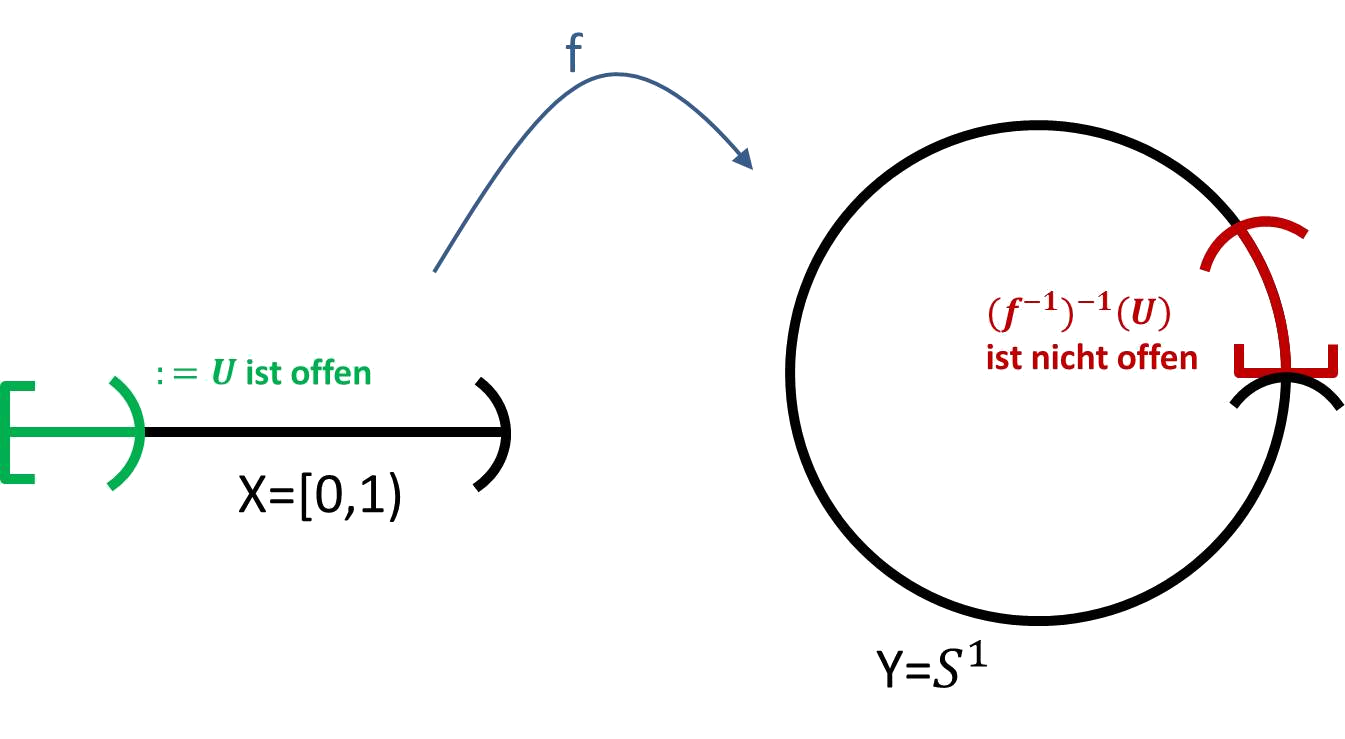
\includegraphics[width=0.5\textwidth]{images/0_1_nach_S1_f-1_nicht_stetig.png}
		\end{center}
		\item $id_X \colon X \rightarrow X$ ist immer ein Homöomorphismus, Kompositionen von Homöomorphismen ebenfalls.
	\end{itemize}
\end{bsp}

\begin{remark}
	`Homöomorph sein' ist eine Äquivalenzrelation für topologische Räume.
\end{remark}

\begin{definition}{homöomorph}
	Zwei topologische Räume $X$ und $Y$ heißen \underline{homöomorph} oder \underline{vom gleichen Homöomorphietyp}, in Zeichen $X \cong Y$, falls es einen Homöomorphismus $f \colon X \rightarrow Y$ gibt.
\end{definition}

\begin{remark}
	Homöomorphismen erhalten sämtliche topologischen Strukturen:
	\begin{itemize}
		\item Ist $f \colon X \rightarrow Y$ Homöomorphismus, so ist $U \subset X$ offen $\Leftrightarrow f(U)$ offen in $Y$.
		\item $A \subset X$ ist abgeschlossen $\Leftrightarrow f(A)$ ist abgeschlossen in $Y$.
		\item $f(\bar{A}) = \overline{f(A)}, f(\mathring A) = \mathring{\left(f(A)\right)}$.
		\item $U$ ist Umgebung von $x \in X$ $\Leftrightarrow f(U)$ ist Umgebung von $f(x)$.
	\end{itemize}
\end{remark}

\begin{bsp}{}
	\begin{itemize}
		\item Jede Isometrie zwischen metrischen Räumen ist ein Homöomorphismus.
		\item $[0,1] \cong [a,b] \forall a < b \in \R$
		\item $(0,1) \cong (a,b) \cong \R \forall a < b \in \R$
	\end{itemize}
\end{bsp}

\begin{bsp}{Stereographische Projektion}
	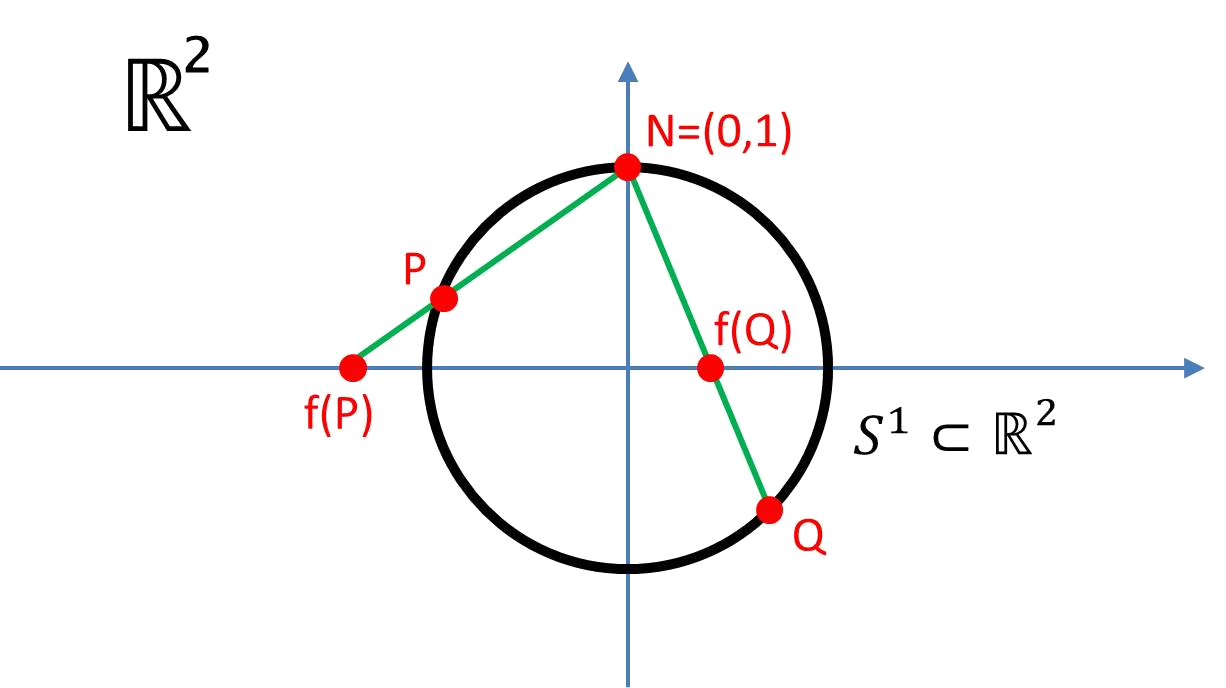
\includegraphics[scale=0.35]{images/Stereographie_S1_R1.png}
	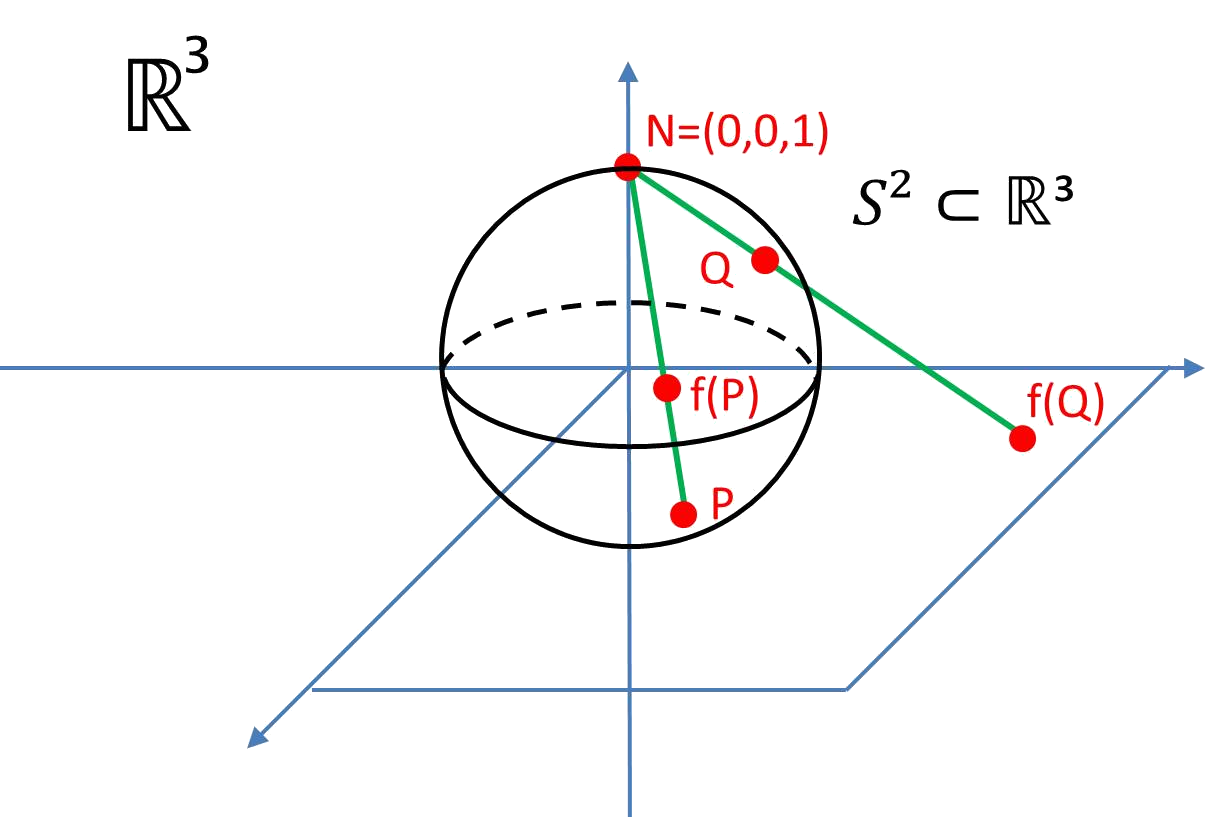
\includegraphics[scale=0.35]{images/Stereographie_S2_R2.png}
	\newline
	Die stereographische Projektion ist ein Homöomorphismus von $S^n \backslash \{N\}, N := (0, \ldots, 0, 1) \in \R^{n+1}$, gegeben wie folgt:
	\newline
	Der Schnitt der Geraden im $\R^{n+1}$ durch $N$ und $x \in S^n \backslash \{N\}$ mit der Hyperebene $\R^n=\{x \in \R^{n+1} \mid x_{n+1} = 0 \}$, $f(x)$, ist gegeben durch $x = (x_1, \ldots, x_{n+1}) \mapsto (\frac{x_1}{1-x_{n+1}}, \frac{x_2}{1-x_{n+1}}, \ldots, \frac{x_n}{1-x_{n+1}}) =: f(x)$ mit Umkehrabbildung $y = (y_1, \ldots, y_n) \mapsto (\frac{2 y_1}{||y||^2+1}, \ldots, \frac{2 y_n}{||y||^2+1},\frac{||y||^2-1}{||y||^2+1})$.
\end{bsp}

\begin{definition}{Einbettung}
	$f \colon X \rightarrow Y$ stetig heißt \underline{Einbettung} $$:\Leftrightarrow X \overset{f}{\rightarrow}f(X) \subset Y \text{ Homöomorphismus.}$$
\end{definition}

\begin{bsp}{}
	\begin{itemize}
		\item Für $A \subset X$ ist die Inklusion $\iota \colon A \hookrightarrow X, x \mapsto x$, stets eine Einbettung.
		\item $[0,1) \rightarrow S^1$ ist \underline{keine} Einbettung!
		\begin{center}
			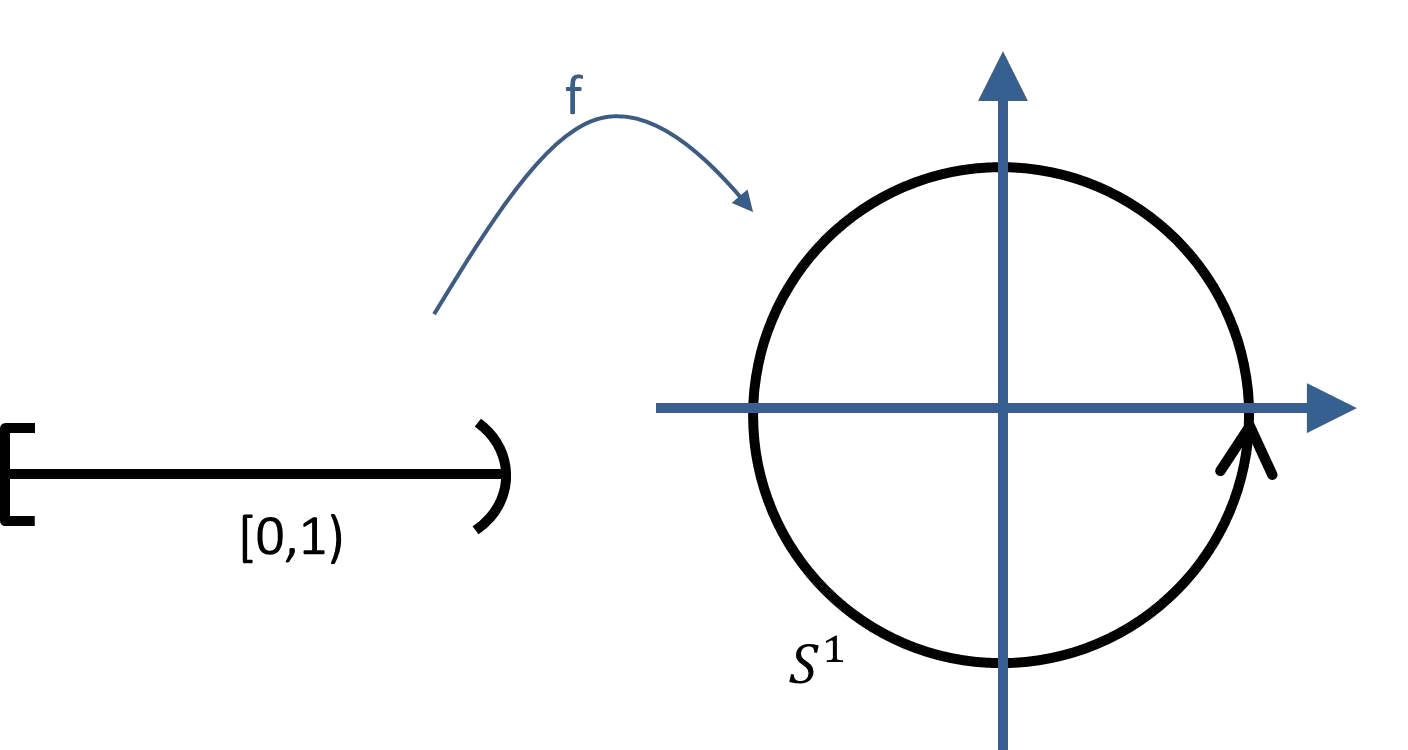
\includegraphics[scale=0.25]{images/0_1_nach_S1_Pfeil.png}
		\end{center}
		\item \underline{Der Satz über die Umkehrabbildung/ Impliziter Funktionensatz} aus der Analysis zeigt: 
			\newline
			Ist $f \colon \R^n \rightarrow \R^n$ stetig differenzierbar und in $p \in \R^n$ die Jacobi-Matrix $Df(p)$ invertierbar, so existiert eine Umgebung von $p$, auf der $f \big |_U$ eine Einbettung ist.
	\end{itemize}
\end{bsp}

\begin{definition}{Äquivalenz von Einbettungen}
	Zwei Einbettungen $f,g \colon X \rightarrow Y$ heißen \underline{äquivalent} $:\Leftrightarrow \exists \text{ Homöomorphismen } h_X \colon X \rightarrow X, h_Y \colon Y \rightarrow Y \text{ mit } g \circ h_X = h_Y \circ f$, d.h. dass das Diagramm 
		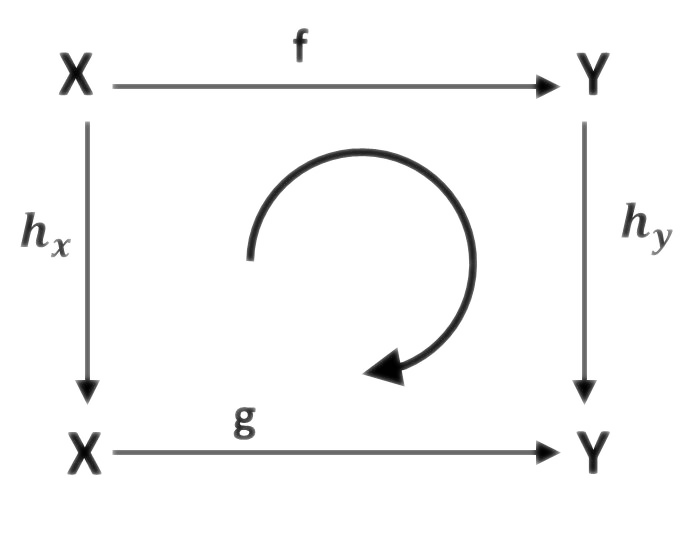
\includegraphics[scale=0.3]{images/homotopieaequivalenz.png} kommutiert.
\end{definition}

\begin{definition}{Knoten}
	Eine Einbettung $S^1 \rightarrow \R^3$ heißt \underline{Knoten}.
\end{definition}

\begin{bsp}{}
	Die Knoten mit Bildern 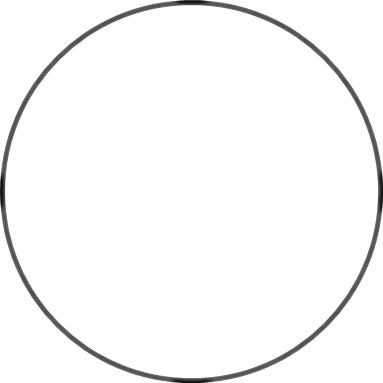
\includegraphics[scale=0.3]{images/Knoten_Kreis.png} und 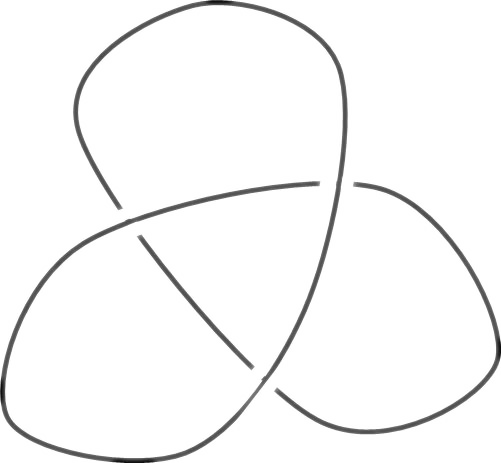
\includegraphics[scale=0.3]{images/Knoten_aequivalent_zu_Kreis.png} sind äquivalent, die mit 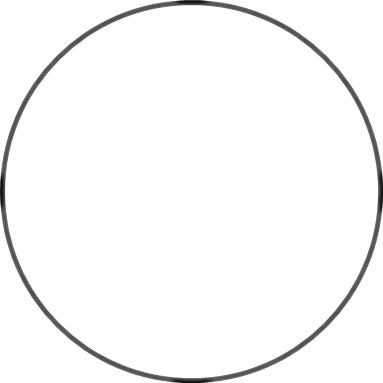
\includegraphics[scale=0.3]{images/Knoten_Kreis.png} und 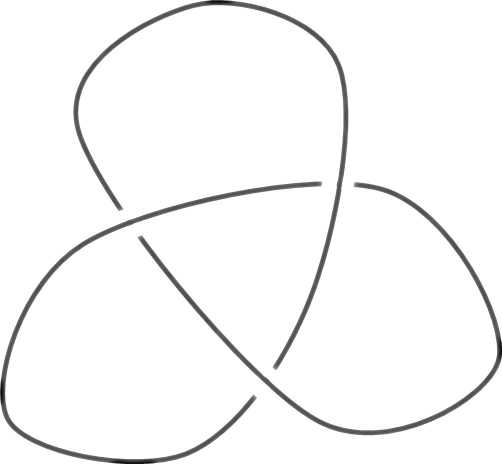
\includegraphics[scale=0.3]{images/Knoten_nicht_aequivalent_zu_Kreis.png} nicht!
\end{bsp}

\section{Zusammenhang und Kompaktheit}

\begin{definition}{zusammenhängend}
	Ein topologischer Raum heißt \underline{zusammenhängend} $:\Leftrightarrow$ Die einzigen in $X$ gleichzeitig offenen und abgeschlossenen Teilmengen sind $\emptyset$ und $X$.
	\newline
	Ansonsten heißt $X$ \underline{un-} oder \underline{nicht zusammenhängend}.
\end{definition}

\begin{definition}{Überdeckung}
	Eine Familie $\mathcal{U} = \{U_\alpha \mid \alpha \in A\}$\footnote{$A$ Indexmenge} von Teilmengen von $X$ heißt \underline{Überdeckung von $X$} $:\Leftrightarrow X = \bigcup\limits_{\alpha \in A}{U_\alpha}$.
	\newline
	$\mathcal{U}$ heißt \underline{offene} beziehungsweise \underline{abgeschlossene} Überdeckung $\Leftrightarrow$ alle $U_\alpha$ sind offen beziehungsweise abgeschlossen.
	\newline
	Für $X^\prime \subset X$ heißt eine Familie $\mathcal{U} = \{U_\alpha\}$ wie oben Überdeckung von $X^\prime$ $:\Leftrightarrow X^\prime \subset \bigcup\limits_{\alpha \in A}{U_\alpha}$.
	\newline
\end{definition}
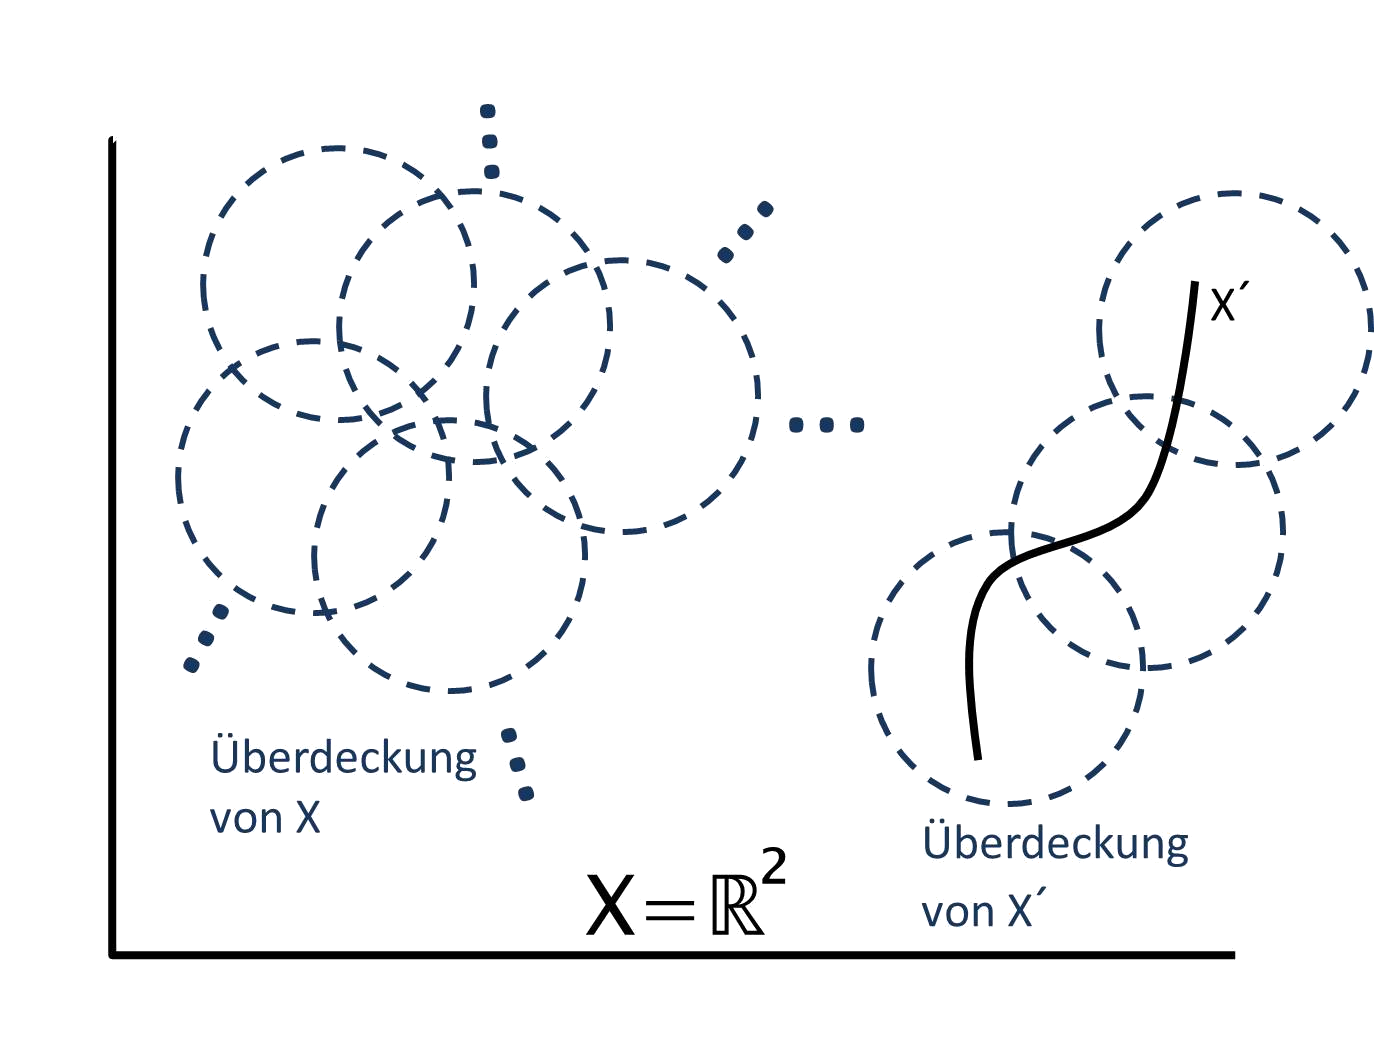
\includegraphics[scale=0.5]{images/Ueberdeckung.png}

\begin{definition}{Partition}
	Eine \underline{Partition} oder \underline{Zerlegung} einer Menge ist eine Überdeckung dieser Menge durch paarweise disjunkte, nichtleere Teilmengen.
	\newline
\end{definition}
\begin{center}
	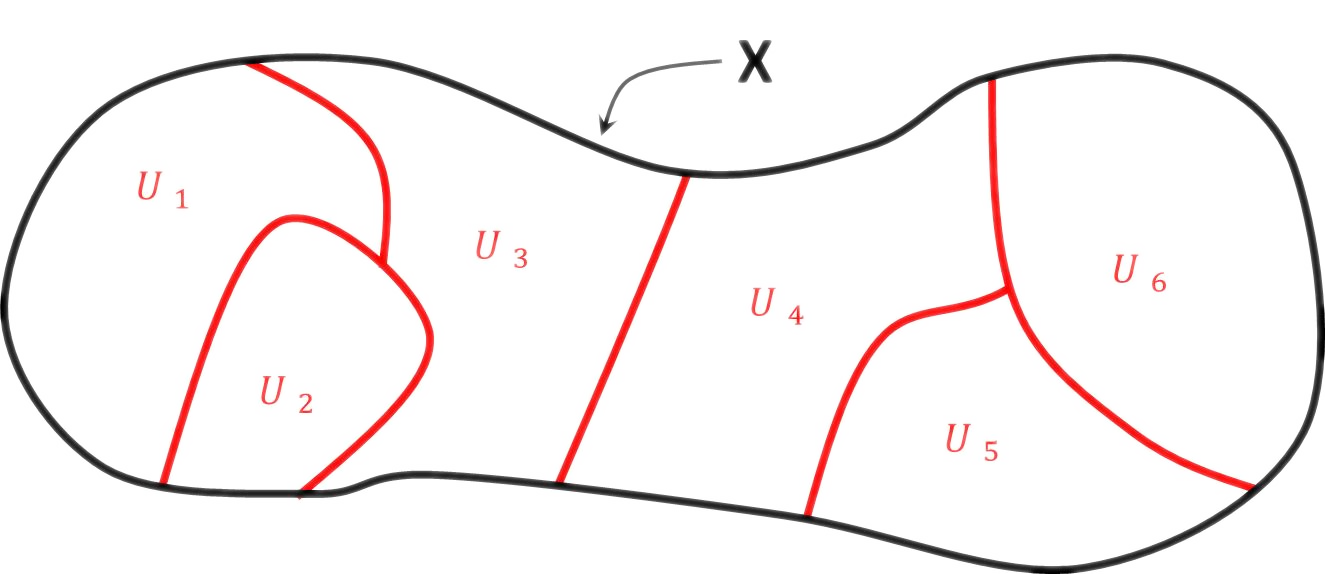
\includegraphics[scale=0.5]{images/Partition.png}
\end{center}

\begin{remark}
	Ein topologischer Raum $X$ ist zusammenhängend 
	$\Leftrightarrow$ Es existiert keine Partition von $X$ in zwei nichtleere offene Teilmengen
	$\Leftrightarrow$ es existiert keine Partition von $X$ in zwei nichtleere abgeschlossene Teilmengen
	\newline
	\underline{Denn:} $A \subset X$ ist offen \underline{und} abgeschlossen
	$\Leftrightarrow$ $A$ und $X \backslash A$ sind offen
	$\Leftrightarrow$ $A$ und $X \backslash A$ sind abgeschlossen
\end{remark}

\begin{bsp}{}
	\begin{itemize}
		\item $\Q$ als Teilmenge von $\R$ ist nicht zusammenhängend, denn $\Q = (\Q \cap (- \infty, \pi)) \cup (\Q \cap (\pi, +\infty)).$
		\item Die einzigen zusammenhängenden und mit der diskreten Topologie versehenen Räume sind $\emptyset$ und der nur aus einem Punkt bestehende Raum.
	\end{itemize}
\end{bsp}

\begin{remark}
	Allgemein sagt man von einer Menge, sie sei zusammenhängend, wenn diese, aufgefasst als Teilraum eines topologischen Raumes, zusammenhängend ist.
\end{remark}

\begin{bsp}{}
	$[0,1] (\subset \R)$ ist zusammenhängend, aber $[0,1] \cup (2,3)$ nicht!
\end{bsp}

\begin{bsp}{}
	Eine Teilmenge $A$ von $\R_{\mathcal{T}_1}$ ist zusammenhängend
	$\Leftrightarrow$ $A$ ist leer, einpunktig, oder unendlich!
\end{bsp}

\begin{remark}{Eigenschaften zusammenhängender Mengen}
	\begin{itemize}
		\item $A$ zusammenhängend $\Rightarrow$ $\bar{A}$ zusammenhängend
		\item $A,B \subset X$ zusammenhängend, $A \cap B \neq \emptyset \Rightarrow A \cup B$ zusammenhängend
		\item $A \cup B$ zusammenhängend, $A \cap B$ zusammenhängend $\not\Rightarrow A,B$ zusammenhängend ($A = \Q, B = \R \backslash \Q$)
	\end{itemize}
\end{remark}

\begin{definition}{Zusammenhangskomponente}
	Eine \underline{Zusammenhangskomponente} eines topologischen Raumes $X$ ist eine im Sinne der Inklusion von Mengen maximale zusammenhängende Teilmenge von $X$.
\end{definition}

\begin{remark}{}
	\begin{itemize}
		\item Jeder Punkt von $X$ liegt genau in einer Zusammenhangskomponente, und diese ist die Vereinigung aller diesen Punkt enthaltenden zusammenhängenden Teilmengen.
		\item Zwei Zusammenhangskomponenten sind damit entweder gleich oder disjunkt.
		\item Zusammenhangskomponenten sind abgeschlossen.
	\end{itemize}
\end{remark}

\begin{theorem}
	Stetige Bilder zusammenhängender Mengen sind zusammenhängend.
	\newline
	(D.h.: Ist $f \colon X \rightarrow Y$ stetig und $X$ zusammenhängend, so auch $f(X)\subset Y$.)
\end{theorem}

\begin{proof}
	Es sei ohne Einschränkung $Y=f(X)$ und sei $Y=U \cup V$ Partition von $Y$ in zwei offene Mengen $\Rightarrow f^{-1}(U), f^{-1}(V)$ sind offen in $X$ ($f$ stetig) und bilden eine Partition von $X$. $X$ ist zusammenhängend.
	$\Rightarrow f^{-1}(U) \text{ oder } f^{-1}(V) = \emptyset$.
	\newline
	Sei o.E. $f^{-1}(U) = \emptyset \Rightarrow U = f(\emptyset) = \emptyset \Rightarrow V = f(X)$ ($f$ surjektiv auf $f(X)$)
	\newline
	$\Rightarrow$ Es existiert \underline{keine} Partition von $Y$ in nichtleere offene Mengen $\Leftrightarrow Y$ zusammenhängend.
\end{proof}

\begin{corollary}
	Zusammenhang bleibt unter Homöomorphismen erhalten, und ebenso die Zahl der Zusammenhangskomponenten.
\end{corollary}

\begin{bsp}{}
	Für $n > 1$ sind $\R^n$ und $\R$ nicht homöomorph!
	\newline
	\underline{Denn:} $\R^n \cong \mathring{D}^n$ (Einheitskugel) und nimmt man aus $\mathring{D}^n$ einen Punkt $p$ heraus, so bleibt für $n>1$ $\mathring{D}^n \backslash \{p\}$ zusammenhängend, $\mathring{D}^1 = (-1,1) \cong \R$ aber nicht!
	\newline
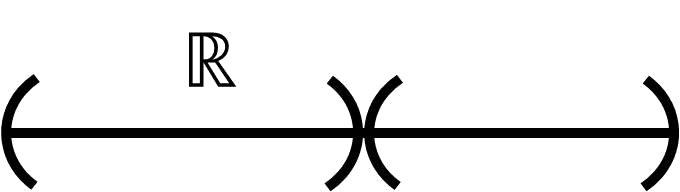
\includegraphics[scale=0.4]{images/R_ohne_p.png}$\qquad\qquad$
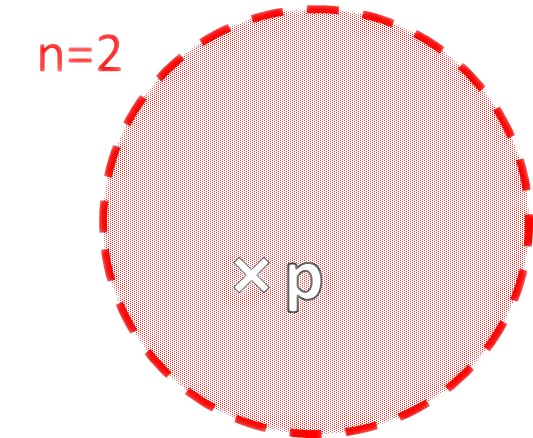
\includegraphics[scale=0.4]{images/R2_ohne_p.png}
	\newline
	\underline{Allgemeiner (Brouwder)} $\R^m \cong \R^n \Leftrightarrow m=n$
\end{bsp}

\begin{corollary}{Zwischenwertsatz:}
	Eine stetige Funktion $f \colon [a,b] \rightarrow \R$ nimmt jeden Wert zwischen $f(a)$ und $f(b)$ an.
\end{corollary}

\begin{bsp}{Waffelteilen}
	Eine Waffel, wie unregelmäßig auch immer, lässt sich immer in zwei gleich große Teile schneiden.
	\newline
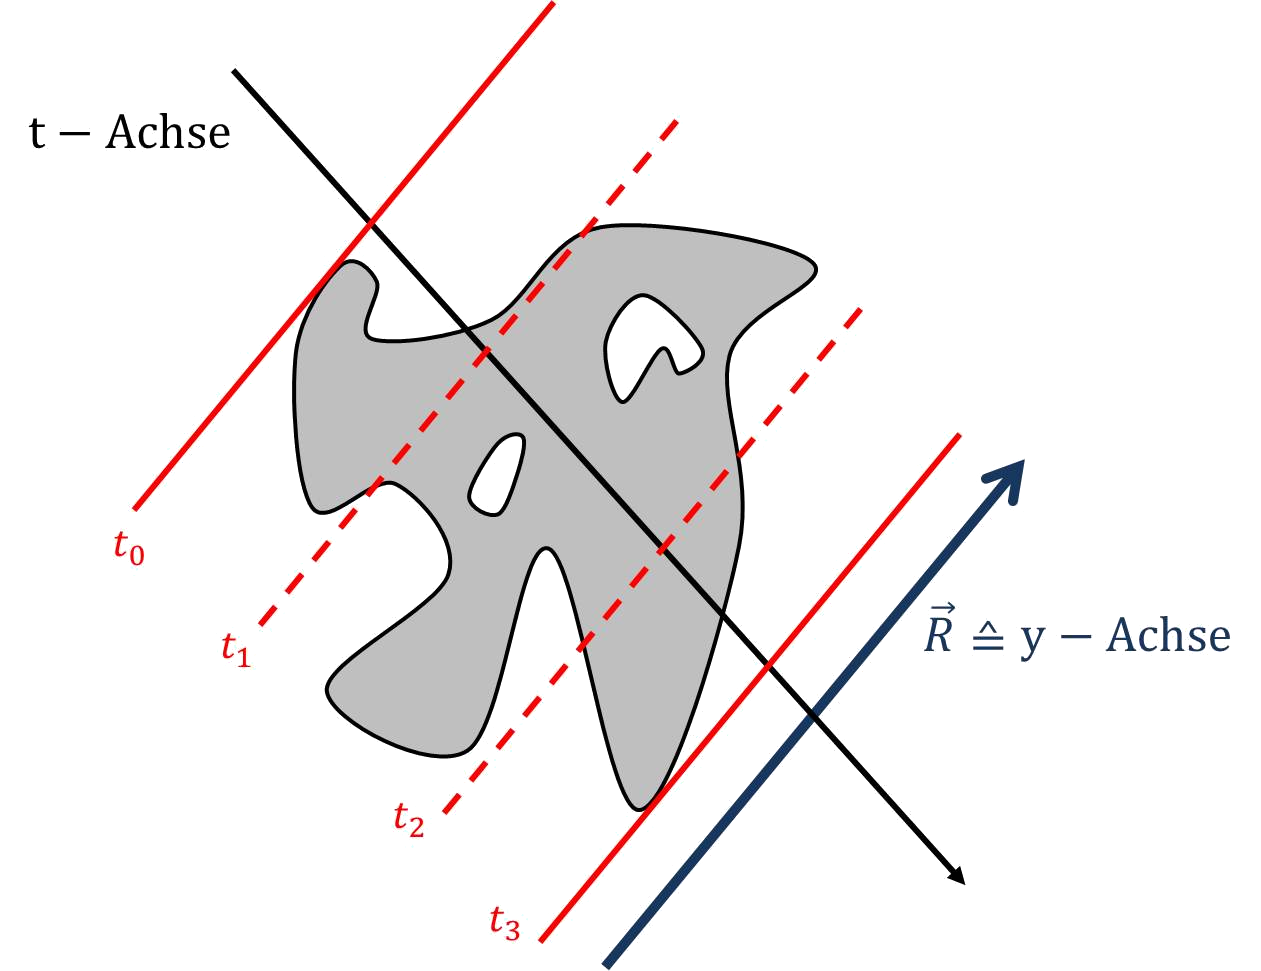
\includegraphics[scale=0.4]{images/Waffel_zshgd.png}
\newline
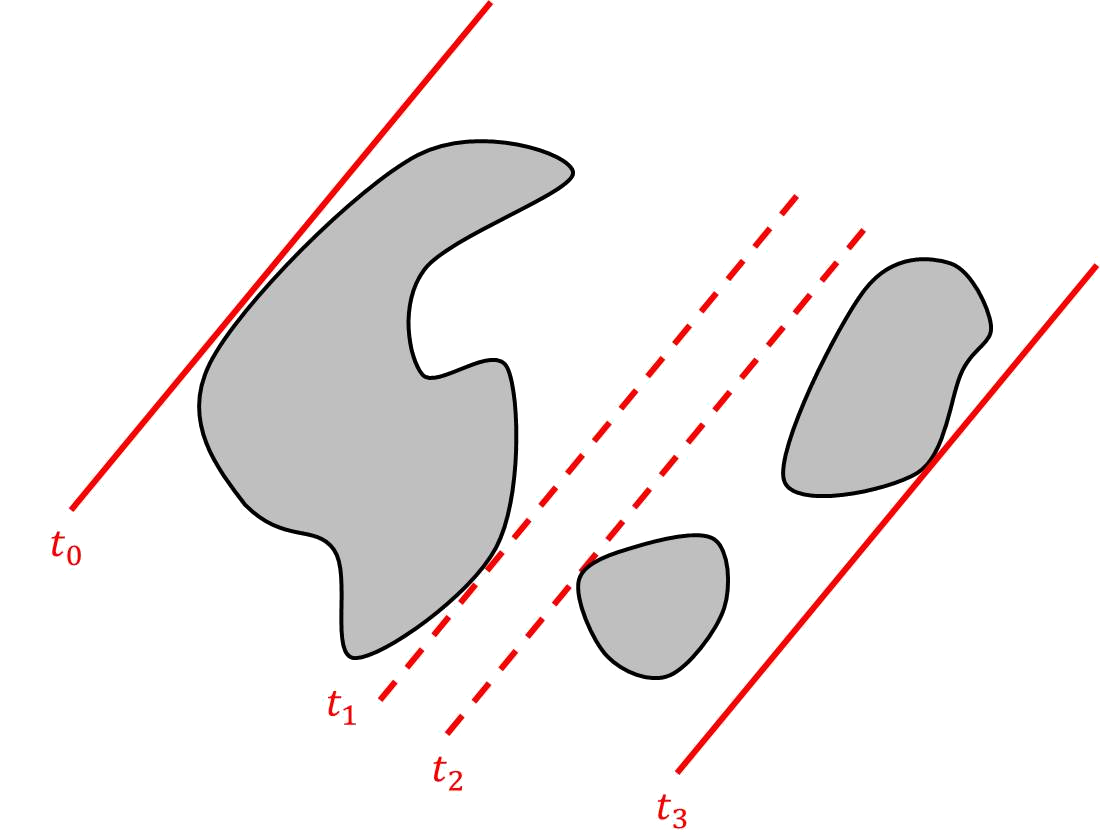
\includegraphics[scale=0.3]{images/Waffel_unzshgd.png} $\qquad$
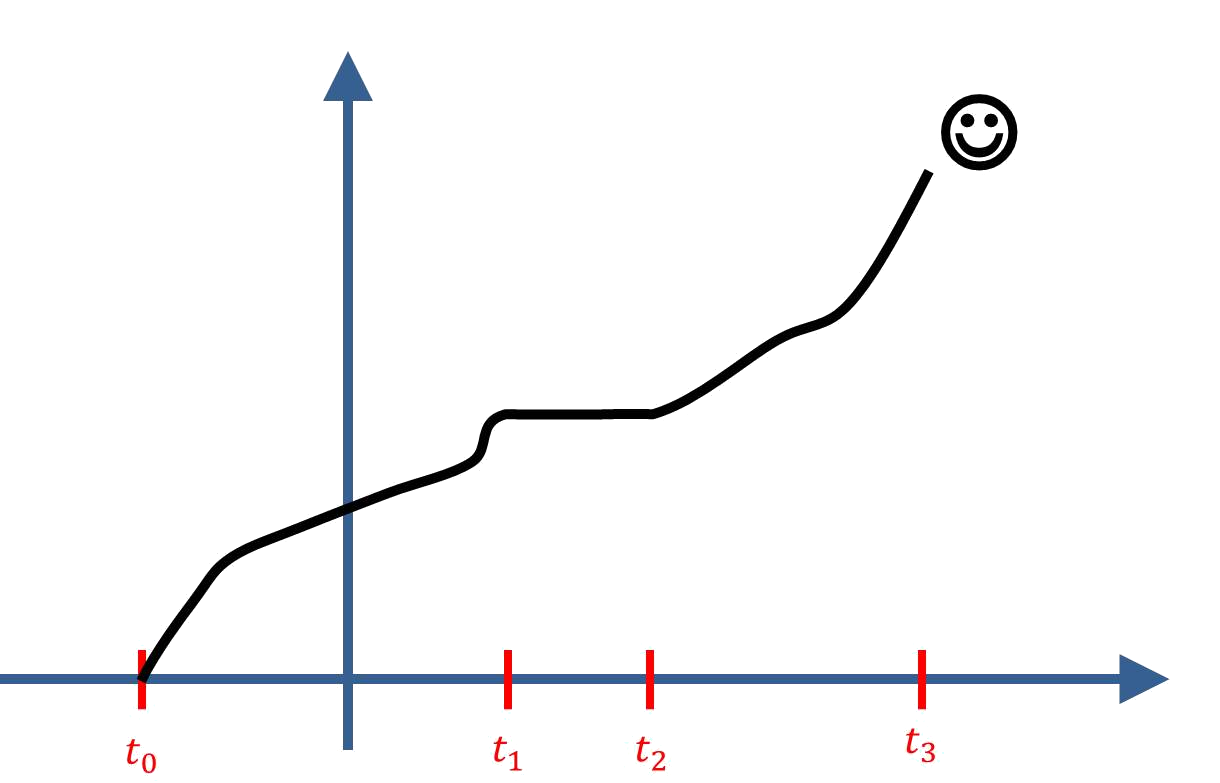
\includegraphics[scale=0.3]{images/Waffel_unzshgd_Fkt.png}
\newline
Bei unzusammenhängenden Waffeln ist die Schnittgerade selbst bei vorgegebener Schnittrichtung nicht eindeutig.
\end{bsp}

\begin{definition}{Weg, Anfangspunkt, Endpunkt}
	ein \underline{Weg} in einem topologischen Raum $X$ ist eine stetige Abbildung $\gamma \colon [0,1] \rightarrow X$, und $\gamma(0)$ heißt \underline{Anfangs-}, $\gamma(1)$ \underline{Endpunkt}.
	\newline
\end{definition}
\begin{center}
	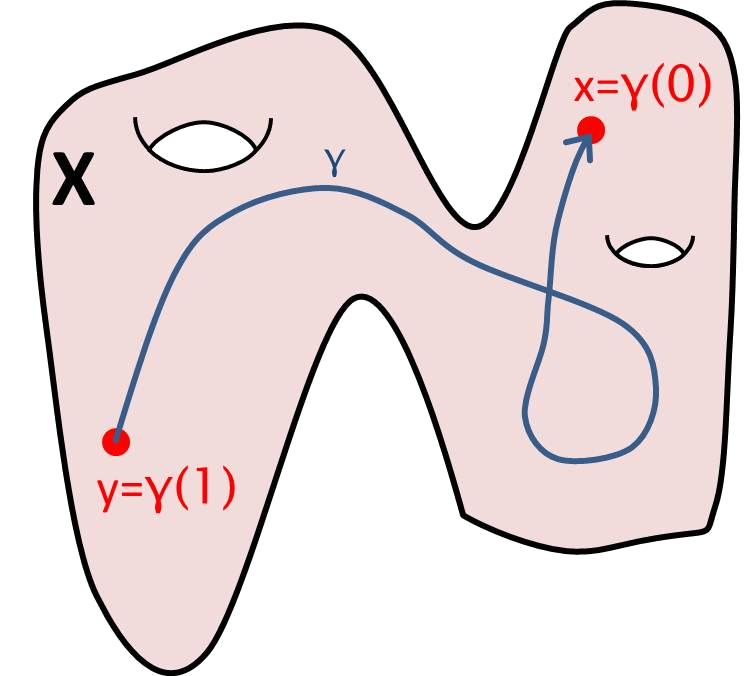
\includegraphics[scale=0.4]{images/Weg.png}
\end{center}

\begin{definition}{Wegzusammenhang}
	$X$ heißt \underline{wegzusammenhängend} $$:\Leftrightarrow \text{ Zu je zwei Punkten } x,x^\prime \in X \quad \exists \text{ Weg } \gamma \colon [0,1] \rightarrow X$$ $$\text{ mit } \gamma(0)=x, \gamma(1)=x^\prime.$$
\end{definition}
\begin{center}
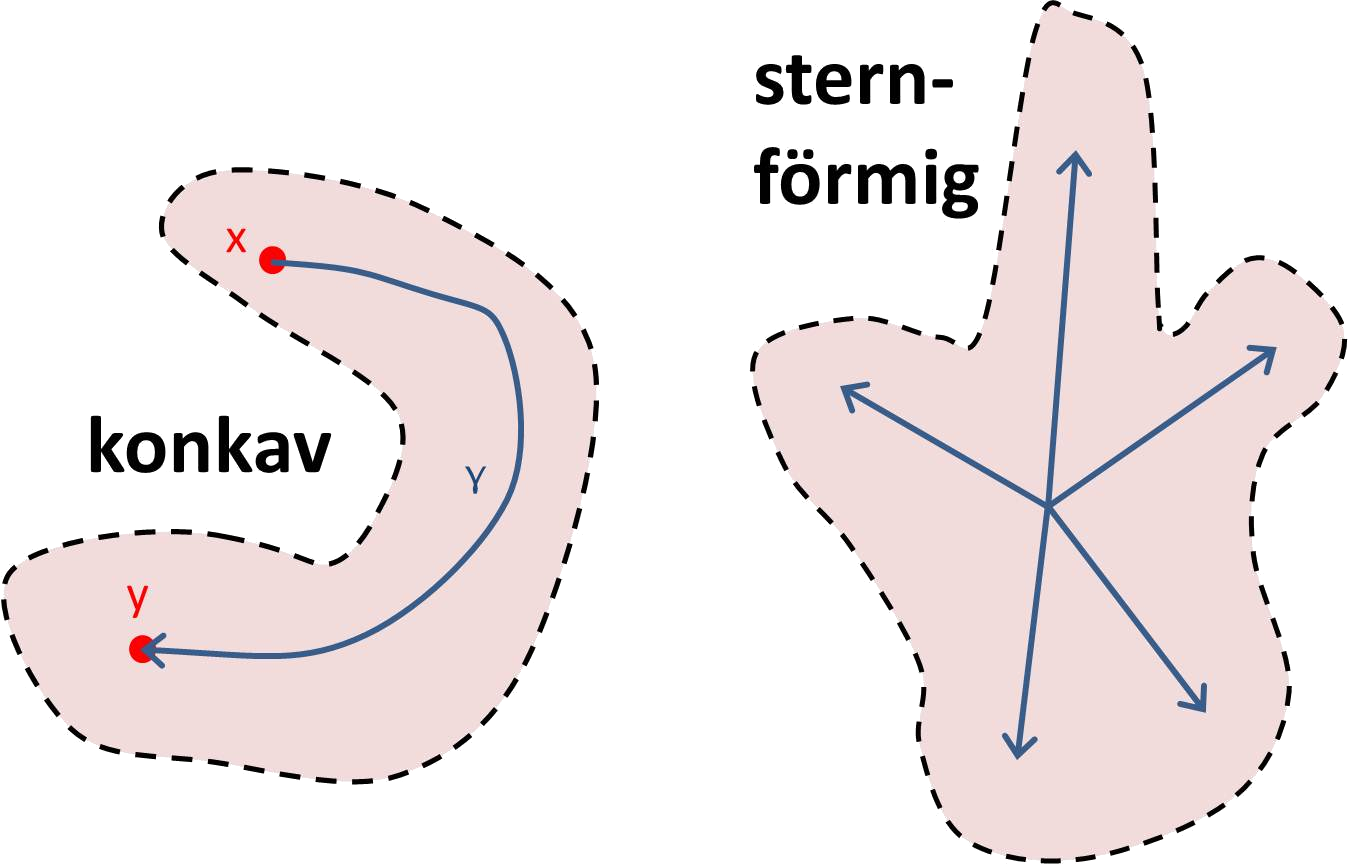
\includegraphics[scale=0.4]{images/Wegzshgd.png}
\end{center}

\begin{bsp}{}
	$$A=\{(x,y) \in \R^2 \mid x>0, y = \sin{\frac{1}{x}}\} \subset \R^2$$
	$$B=A \cup \{(0,0)\}$$
	$\Rightarrow B$ ist zusammenhängend, aber \underline{nicht} wegzusammenhängend.
	\newline
	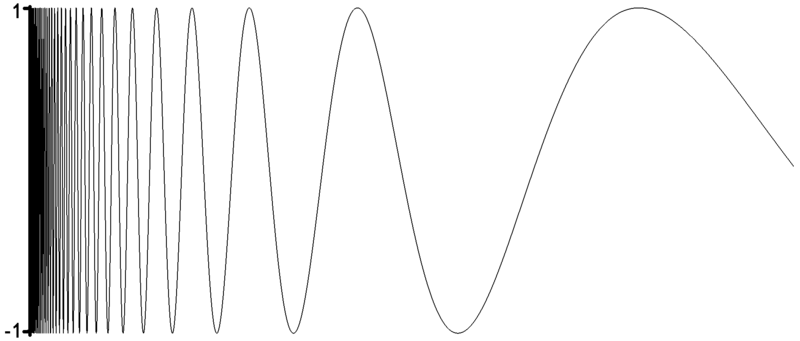
\includegraphics[scale=0.4]{images/Sinuseinsdurchx.png}
	\newline
	\scriptsize{Bild: http://de.wikipedia.org/w/index.php?title=Datei:Sinuseinsdurchx.png\&filetimestamp=20080624085708}
\end{bsp}

\begin{definition}{Kompaktheit}
	Ein topologischer Raum $X$ heißt \underline{kompakt}, falls jede offene Überdeckung von $X$ eine endliche Teilüberdeckung enthält.
\end{definition}

\section{Trennungseigenschaften}
\begin{definition}{$T_1$-Raum}
Ein topologischer Raum $X$ heißt \underline{$T_1$-Raum} bzw. \underline{erfüllt das erste Trennungsaxiom} $:\Leftrightarrow$ Für je zwei verschiedene Punkte von $X$ existiert für jeden dieser Punkte eine Umgebung in $X$, die den anderen nicht enthält.
\newline
$\forall x \neq y \in X \exists U = U_X \colon y \notin U_X$ 
\end{definition}
\begin{center}
\includegraphics[scale=0.4]{images/T1.png}
\end{center}

\begin{definition}{$T_2$-Raum}
	$X$ heißt \underline{Hausdorff}- oder \underline{$T_2$-Raum} bzw. \underline{erfüllt das zweite Trennungsaxiom} $:\Leftrightarrow$ Je zwei verschiedene Punkte in $X$ besitzen disjunkte Umgebungen.
	\newline
	$\forall x \neq y \in X \exists U_x \ni x, U_y \ni y$ mit $U_x \cap U_y = \emptyset$
\end{definition}
\begin{center}
\includegraphics[scale=0.4]{images/T2.png}
\end{center}

\begin{bsp}{}
	Jeder metrische Raum ist Hausdorff-Raum.
\end{bsp}

\begin{remark}
Hausdorff-Räume sind z.B. deshalb wichtig, weil Grenzwerte dort eindeutig sind!
\end{remark}

\begin{definition}{Grenzwert}
Ist $(x_n)_{n \in \N}$ eine Folge von Punkten in einem topologischen Raum $X$, so heißt $x \in X$ \underline{Grenzwert} der Folge $(x_n)$ genau dann, wenn zu jeder Umgebung $U$ von $x$ ein $N \in \N$ existiert mit $x_n \in U \quad \forall n \geq N$. 
\newline
\end{definition}
\begin{center}
	\includegraphics[scale=0.5]{images/Grenzwert.png}
\end{center}

\begin{bsp}{}
In einem Hausdorff-Raum hat jede Folge höchstens einen Grenzwert.
\end{bsp}

\begin{remark}
Hausdorff-Räume sind auch $T_1$-Räume, aber:
\end{remark}

\begin{bsp}{}
	In $X=\R_{\mathcal{T}_1}$ ist jeder Punkt abgeschlossen ($\Rightarrow T_1$), doch je zwei nichtleere offene Mengen schneiden sich - $X$ ist damit nicht $T_2$!
	%newline
	\underline{"Schlimmer":} In $\R_{\mathcal{T}_1}$ ist \underline{jeder} Punkt Grenzwert der Folge $x_n = n$!
	Denn eine Umgebung eines Punktes in $\R_{\mathcal{T}_1}$ hat die Form $U = \R \backslash \{x_1, \ldots, x_M\}$ mit $x_1 < \ldots < x_M$. Dann gilt aber $x_n = n \in U \forall n > x_M$.
\end{bsp}

\newpage
\section{Abzählbarkeitsaxiome und lokale Kompaktheit}
\begin{definition}{Umgebungsbasis}
	Ist $X$ topologischer Raum und $x \in X$, so ist eine \underline{Umgebungsbasis} oder \underline{Basis von $X$} \underline{\underline{in $x$}} eine Familie von Umgebungen von $x$, sodass \underline{jede} Umgebung von $x$ eine Umgebung aus der Familie enthält.
\end{definition}

\begin{bsp}{}
	Ist $B$ Basis der Topologie eines Raumes $X$, so ist für jedes $x \in X$ $\{U \in B \mid x \in U\}$ eine Basis von $X$ \underline{\underline{in $x$}}.
\end{bsp}

\begin{bsp}{}
	In einem \underline{metrischen} Raum $X$ sind folgende Mengen von Bällen Basen von $X$ in $x \in X$:
	\begin{itemize}
		\item alle offenen Bälle mit Zentrum $x$
		\item alle offenen Bälle mit Zentrum $x$ und rationalen Radii
	\end{itemize}
\end{bsp}

\begin{bsp}{}
	\label{UmgebungsbasisDiskreteTopologie}
	Ist $X$ mit der diskreten bzw. trivialen Topologie versehen, so ist die `kleinste' Basis in $x \in X$ gegeben durch $\left\{\{x\}\right\}$ bzw. $\{X\}$.
\end{bsp}

\begin{definition}{Abzählbarkeitsaxiome, Separabilität}
	$X$ \underline{erfüllt das erste Abzählbarkeitsaxiom}
	$:\Leftrightarrow$ jeder Punkt $x \in X$ besitzt eine abzählbare Basis.
	\newline
	$X$ \underline{erfüllt das zweite Abzählbarkeitsaxiom}
	$:\Leftrightarrow$ $X$ selbst besitzt eine abzählbare Basis.
	\newline
	$X$ heißt \underline{separabel} $:\Leftrightarrow$ $X$ enthält eine abzählbare und dichte ($\bar{A} = X$) Menge $A$.
\end{definition}
 
\begin{remark}
	Das zweite Abzählbarkeitsaxiom impliziert das erste, aber:
\end{remark} 

\begin{bsp}{}
	Überabzählbare diskrete Räume (wie $(\R, \OO_{diskret})$) erfüllen nach Beispiel~\ref{UmgebungsbasisDiskreteTopologie} das erste Abzählbarkeitsaxiom, nicht aber das zweite!
\end{bsp}
 
\begin{remark}
	Jeder metrische Raum erfüllt das erste Abzählbarkeitsaxiom und jeder \underline{separable} metrische Raum auch das zweite.
\end{remark} 
 
\begin{bsp}{}
	$\R_{\mathcal{T}_1}$ erfüllt \underline{nicht} das erste Abzählbarkeitsaxiom, ist aber separabel - $\N$ ist dicht!
\end{bsp} 
 
\begin{bsp}{}
	Euklidische Räume und alle ihre Teilmengen erfüllen das 2. Abzählbarkeitsaxiom und sind separabel.
\end{bsp} 
 
Wozu das Ganze? 
\newline $\rightsquigarrow$ Funktionenräume
\newline $\rightsquigarrow$ Mannigfaltigkeiten
\newline $\rightsquigarrow$ \underline{Satz von Lindelöf:}
Jede offene Überdeckung eines Raumes, der das zweite Abzählbarkeitsaxiom erfüllt, enthält auch eine abzählbare \underline{Teilüberdeckung}.
 
\begin{definition}{Lokale Kompaktheit}
$X$ heißt \underline{\underline{lokal} kompakt} \newline $:\Leftrightarrow$ Jeder Punkt $x \in X$ besitzt eine Umgebung $U$, sodass $\overline{U}$ kompakt ist.
\end{definition} 

\begin{definition}{Lokale Endlichkeit}
	Eine Familie $\Gamma$ von Teilmengen eines topologischen Raumes $X$ heißt \underline{lokal endlich} $:\Leftrightarrow \forall x \in X \quad \exists U = U(x) \colon A \cap U = \emptyset \quad \forall A \in \Gamma$ bis auf endlich viele $A$.
\end{definition}
\begin{center}
	\includegraphics[scale=0.5]{images/lokal_endlich.png}
\end{center} 
 
\begin{definition}{Verfeinerung}
	$\Gamma, \Delta$ Überdeckungen von $X$. $\Delta$ heißt \underline{Verfeinerung} von $\Gamma$ \newline $:\Leftrightarrow \forall A \in \Delta \exists B \in \Gamma \colon A \subset B$.
\end{definition} 

\begin{definition}{Parakompaktheit}
	$X$ heißt \underline{parakompakt} $:\Leftrightarrow$ Jede offene Überdeckung besitzt eine lokal endliche offene Verfeinerung. 
\end{definition}

\includegraphics[scale=0.5]{images/Cutoff.png} \underline{\underline{Cut-off}}

\begin{bsp}{}
	 \begin{itemize}
	 	\item Kompakte Räume sind parakompakt.
	 	\item $\R^n$ ist parakompakt.
	 	\item Mannigfaltigkeiten sind parakompakt!
	 \end{itemize}
\end{bsp}

\begin{remark}{}
	Parakompaktheit ist wichtig, da dann bestimmte Einbettungen und sogenannte Zerlegungen der Eins existieren.
\end{remark}

%hier beginnt der 10.11.11
\chapter{Geometrische Beispiele und Konstruktionen topologischer Räume}
\section{Mannigfaltigkeiten}

\paragraph{Beispiele zu Mannigfaltigkeiten (Exkurs)} Doppelpendel, Quantenfeldtheorie

\includegraphics[scale=0.3]{images/Mannigfaltigkeiten1.png} \newline \newline
\includegraphics[scale=0.4]{images/S1_Pendel.png} \newline \newline
\includegraphics[scale=0.4]{images/Torus_Doppelpendel.png} \newline \newline
\includegraphics[scale=0.4]{images/Stringtheorie.png}

\begin{definition}{Mannigfaltigkeit, Karte}
	Ein topologischer Raum $M$ heißt \underline{$n$-dimensionale} \underline{(topologische) Mannigfaltigkeit}, wenn gilt:
	\begin{enumerate}
		\item $M$ ist ein Hausdorff-Raum mit abzählbarer Basis der Topologie
		\item $M$ ist lokal homöomorph zu $\R^n$, d.h. zu jedem $p \in M$ existieren eine Umgebung $U=U(p) \subset_{offen} M$ und ein Homöomorphismus $\varphi \colon U \rightarrow V, V \subset_{offen} \R^n$.
			\newline
			Jedes solche Paar $(U,\varphi)$ heißt eine \underline{Karte} oder ein \underline{lokales Koordinatensystem} um $p$.
	\end{enumerate}
\end{definition}
\begin{center}
	\includegraphics[scale=0.4]{images/Karte.png} 
\end{center} 
 
\begin{remark}
	Die Zahl $n$, die \underline{Dimension von $M$}, ist eindeutig bestimmt!
	(folgt aus Brouwers Satz von der Invarianz des Gebietes) 
\end{remark}

\begin{definition}{Atlas}
	Ein \underline{Atlas} für eine topologische $n$-Mannigfaltigkeit $M$ ist eine Menge $\mathcal{A} = \{(\varphi_\alpha, U_\alpha) \mid \alpha \in \Lambda\}$\footnote{$\Lambda$ Indexmenge}
	von Karten $\varphi_\alpha \colon U_\alpha \rightarrow V_\alpha = \varphi(U_\alpha) \subset \R^n$, so dass $M = \bigcup\limits_{a \in \Lambda}{U_\alpha}$
\end{definition}

\begin{definition}{$C^k$-Atlas, Kartenwechsel}
	Ein Atlas heißt \underline{differenzierbar} \underline{von der Klasse $C^k$} (oder: $C^k$-Atlas von $M$), wenn für alle $\alpha, \beta \in \Lambda$ mit $U_\alpha \cap U_\beta \neq \emptyset$ der \underline{Kartenwechsel} $\varphi_\beta \circ \varphi_\alpha^{-1} \colon \varphi_\alpha(U_\alpha \cap U_\beta) \rightarrow \varphi_\beta(U_\alpha \cap U_\beta)$ eine $C^k$-Abbildung, also $k$-mal stetig differenzierbar ist. $(k=0,1,2,\ldots,\infty,\omega)$
	\newline
\end{definition}
\begin{center}
	\includegraphics[scale=0.4]{images/Kartenwechsel.png}
\end{center} 
 
\begin{definition}{Verträglichkeit, differenzierbare Struktur}
	Ist $M$ topologische Mannigfaltigkeit und $\mathcal{A}=\{(\varphi_\alpha,U_\alpha) \mid \alpha \in \Lambda\}$ ein $C^k$-Atlas von $M$, so heißt eine Karte $(\varphi,U)$ von $M$ \underline{mit $\mathcal{A}$ verträglich}, falls $\mathcal{A}^\prime := \mathcal{A} \cup \{(\varphi,U)\}$ ebenfalls $C^k$-Atlas ist. 
	Ein $C^k$-Atlas heißt \underline{maximal} (oder \underline{differenzierbare Struktur} (der Klasse $C^k$)), falls $\mathcal{A}$ alle mit $\mathcal{A}$ verträglichen Karten enthält.
\end{definition} 

\begin{definition}{$C^k$-Mannigfaltigkeit, glatt}
	Eine \underline{differenzierbare Mannigfaltigkeit der Klasse $C^k$} (kurz: $C^k$-Mannigfaltigkeit) ist ein Paar $(M,\mathcal{A})$ bestehend aus einer topologischen Mannigfaltigkeit $M$ und einer $C^k$-Struktur auf $M$. Eine $C^\infty$-Mannigfaltigkeit heißt auch \underline{\underline{glatt}}.
	\newline
\end{definition}
\includegraphics[scale=0.4]{images/Verkleben.png}
\includegraphics[scale=0.4]{images/Verkleben_S2.png}
\includegraphics[scale=0.4]{images/Norm_invers.png}


\paragraph{Richtig toller Exkurs zu Mannigfaltigkeiten}... Killing-Fields, Lie-Groups (festgenommener Matheprof kurz nach 9/11), Perverse Garben, wir leben in einer 4-dimensionalen Mannigfaltigkeit, ...

\newpage
\begin{remark}{Bemerkung zur Produkt-Topologie}
\begin{itemize}
	\item Produkte von Hausdorff-Räumen sind Hausdorff-Räume.
	\item Produkte von zusammenhängenden Räumen sind zusammenhängend.
	\item Produkte von wegzusammenhängenden Räumen sind wegzusammenhängend.
	\item Produkte von kompakten/separablen Räumen sind kompakt/separabel.
	\item Produkte von Räumen, die das erste oder zweite Abzählbarkeitsaxiom erfüllen, erfüllen diese auch.
\end{itemize}
 
\paragraph{Folgerung}
	Produkte topologischer oder differenzierbarer Mannigfaltigkeiten sind topologische oder differenzierbare\footnote{($C^\infty$)} Mannigfaltigkeiten.
\end{remark}
 
\begin{bsp}{}
	\begin{itemize}
		\item $\R^2 \backslash \{0\} \cong S^1 \times \R^{> 0}$ (Polarkoordinaten) \newline
		\begin{center}		
			\includegraphics[scale=0.4]{images/Polarkoordinaten.png}
		\end{center}
		\item $O(n) \cong SO(n) \times O(1)$
		\item $(S^1)^n :=  \underbrace{S^1 \times \ldots \times S^1}_{\text{n mal}}$ heißt \underline{n-dimensionaler Torus} (TODO: Bild 3: Exkurs höherdimensionale Sphären)
	\end{itemize}
\end{bsp}

\newpage
\subsection{Differenzierbare Abbildungen}
\begin{definition}{$C^l$-Abbildung}
Es seien $(M, \mathcal{A})$ eine $n$-dimensionale $C^k$-Mannigfaltigkeit, $(M^\prime, \mathcal{A}^\prime)$ eine $n^\prime$-dimensionale $C^{k^\prime}$-Mannigfaltigkeit und $l \leq \min(k,k^\prime)$. Eine stetige Abbildung $f \colon M \rightarrow M^\prime$ heißt \underline{differenzierbar} (\underline{von der Klasse $C^l$}) oder kurz: $C^l$-Abbildung, falls gilt:
$$\forall (\varphi,U) \in \mathcal{A} \text{ und } (\varphi^\prime, U^\prime) \in \mathcal{A}^\prime \text{ mit } f(U) \cap U^\prime \neq \emptyset \text{ ist}$$
$$\boxed{\varphi^\prime \circ f \circ \varphi^{-1} \colon \varphi(U \cap f^{-1}(U^\prime)) \rightarrow \varphi^\prime(f(U)\cap U^\prime)}$$
eine $C^l$-Abbildung im üblichen Sinn.
\end{definition}
\begin{center}
	\includegraphics[scale=0.5]{images/Abb_diffbar.png}
\end{center}

TODO: Exkurs über Tangentialvektoren, Vektorfelder, Satz vom Igel, Physik des starren Körpers, Differentialtopologie

\newpage 
\paragraph{
Spezielle Mannigfaltigkeiten: Untermannigfaltigkeiten topologischer Räume: }
 
\begin{theorem}[Äquivalente Beschreibungen einer Untermannigfaltigkeit von $\R^{n+l}$]
	Für Teilmengen $M \subset \R^{n+l}$ sind äquivalent:
	\begin{enumerate}[(a)]
		\item $\forall x_0 \in M \exists \text{ Umgebung } U = U(x_0) \subset_{offen} \R^{n+l}$ und $$f \in C^\infty(U, \R^l) := \{g \colon U \rightarrow \R^l \mid g \text{ ist } C^\infty\}\text{ mit Rang }Df(x) = l \quad \forall x \in U$$ \footnote{$Df$ ist die Jacobi-Matrix von $f$} dergestalt, dass $U \cap M = f^{-1}(0) = \{x \in U \mid f(x) = 0\}$ 
	\begin{center}
\includegraphics[scale=0.5]{images/Satz_UnterMf.png}
	\end{center}
		\item $\forall x_0 \in M \exists U = U(x) \subset_{offen} \R^{n+l}$ und $\varphi \colon U \rightarrow \R^{n+l}$ mit folgenden Eigenschaften:
		$\varphi(U) \subset \R^{n+l}$ ist offen, \newline $\varphi$ ist $C^\infty$-Diffeomorphismus $U \rightarrow \varphi(U)$ und $$\varphi(U \cap M) = \varphi(U) \cap (\R^n \times \{0\}) = \{(y_1, \ldots, y_{n+l}) \in \varphi(U) \mid y_{n+1} = \ldots = y_{n+l} = 0 \}$$
		\item $\forall x_0 \in M \exists U = U(x_0) \subset_{offen} \R^{n+l}, W \subset \R^n$ offen und $\psi \in C^\infty(W,U)$ mit 
			\begin{itemize}
				\item $\psi$ ist Homöomorphismus $W \rightarrow U \cap M$
				\item $D\psi(w)$ ist injektiv für alle $w \in W$
			\end{itemize}
			(Jedes solche $\psi$ heißt \underline{lokale Parametrisierung von $M$}).
	\end{enumerate}
\end{theorem}

\paragraph{Interpretation}
\begin{enumerate}[(a)]
	\item besagt: $U \cap M$ ist (im Sinne der Rangbedingung) durch $l$ unabhängige Gleichungen $f_1(x) = \ldots = f_l(x) = 0$ definiert.
	\item besagt: nach Anwendung eines Diffeomorphismus sieht $U \cap M$ wie eine offene Teilmenge eines linearen Unterraumes von $\R^{n+l}$ aus.
	\item besagt: $M$ lässt sich lokal parametrisieren.
\end{enumerate}

\begin{definition}{Untermannigfaltigkeit}
Eine Menge $M \subset \R^{n+l}$, die eine der Bedingungen (a), (b) oder (c) erfüllt, heißt dann \underline{$n$-dimensionale} \underline{(glatte/differenzierbare) Untermannigfaltigkeit von $\R^{n+l}$}.
\end{definition}

%hier beginnt der 17.11.

\begin{theorem}{Äquivalente Beschreibung einer glatten Untermannigfaltigkeit von $\R^{n+l}$}
	Es sei $M \subseteq \R^{n+l}$. Es sind äquivalent:
	\begin{enumerate}[(a)]
		\item $\forall x_0 \in M \exists U = U(x_0) \subseteq_{\text{offen}} \R^{n+l} \text{ und } f \in C^\infty(U,\R^l)$ $\text{ mit Rang }Df(x) = l \text{ für alle } x \in U$ dergestalt, dass $U \cap M = f^{-1}(0)$.
		\item $\forall x_0 \in M \exists U = U(x) \subseteq_{\text{offen}} \R^{n+l} \text{ und } \varphi \colon U \rightarrow \R^{n+l}$ mit folgenden Eigenschaften:
			\begin{itemize}
				\item $\varphi(U) \subseteq \R^{n+l}$ ist offen
				\item $\varphi$ ist $C^\infty$-Diffeomorphismus $U \rightarrow \varphi(U)$
				\item $\varphi(U \cap M) = \varphi(U) \cap (\R^n \times \{0\})$ $= \{(y_1, \ldots, y_n) \in \varphi(U) \mid y_{n+1} = \ldots = y_{n+l} = 0\}$
			\end{itemize}
		\item $\forall x_0 \in M \exists U = U(x_0) \subseteq_{\text{offen}} \R^{n+l}$, $W \subseteq \R^n$ offen und $\psi \in C^\infty(W,U)$ mit folgenden Eigenschaften:
			\begin{itemize}
				\item $\psi$ ist Homöomorphismus $W \rightarrow U \cap M$
				\item $D\psi(w)$ ist injektiv für alle $w \in W$.
			\end{itemize}
	\end{enumerate}
\end{theorem}

\begin{bsp}{}
	\underline{zu (a)}
	\newline
	Die $n$-Sphäre vom Radius $r$ %TODO: r=0, r<0?
	$$S_r^n = \{x \in \R^{n+1} \mid ||x|| = r\}$$
	ist eine $n$-dimensionale glatte Untermannigfaltigkeit von $\R^{n+1}$.
	\newline
	\underline{Denn:}
	Definiere $f \colon \R^{n+1} \rightarrow \R, x \mapsto ||x||^2 - r^2$.
	Dann gilt:
	\begin{itemize}
		\item $S_r^n = f^{-1}(0)$ und
		\item $Df(x) = (2x_1, \ldots, 2x_{n+1}) = 2x$
	erfüllt Rang $Df(x)=1$ für alle $x \in \R^{n+1}\backslash\{0\} \supseteq S_r^n$ (wegen $||x||=\sqrt{x_1^2+\dotsb+x_{n+1}^2}$).
		\end{itemize}
		
	Allgemeiner:
	\begin{itemize}
		\item \underline{Niveaumengen:}
			Es seien $V \subseteq_{\text{offen}} \R^{n+l}, f \in C^\infty(V, \R^l), c \in \R^l$.
			Gilt Rang $Df(x) = l$ in jedem Punkt $x$ der \underline{Niveaumenge} $$f^{-1}(c)=\{x \in V \mid f(x)=c\},$$ so ist $f^{-1}(c)$ eine glatte $n$-dimensionale Untermannigfaltigkeit von $\R^{n+l}$.
	\end{itemize}
\end{bsp}

\begin{proof}
		\underline{(a)$\Rightarrow$(b):} Es seien $U$ und $f$ wie in (a) gewählt und $f_1, \ldots, f_l$ die Komponenten von $f$. Sei $x_0 \in M$. Durch Umnummerierung seien die Indizes so gewählt, dass ohne Einschränkung die Reihenfolge so, dass die $(l \times l)$-Matrix 
		$$\left(\frac{\partial f_i}{\partial x_{n+j}}\right)_{i,j \in \{1, \ldots, l\}}$$
		in $x_0$ invertierbar ist.
		Definiere die Abbildung $\varphi \colon U \rightarrow \R^{n+l}, x \mapsto (x_1, \ldots, x_n, f_1(x), \ldots, f_l(x))$.
		Dann gilt:
		$$D \varphi(x_0)= (TODO:Matrix 2)$$ und damit 
		$$\det{D \varphi(x_0)} = \det{\left(\frac{\partial f_i}{\partial x_{n+j}}\right)_{i,j}} \neq 0.$$
		Mit dem Satz über inverse Funktionen (oder "Satz über die Umkehrabbildung") folgt:
		Es existieren Umgebungen $U^\prime = U^\prime(x_0) \subseteq U$ und $V^\prime(\varphi(x_0)) \subseteq V = \varphi(U)$, so dass
		$\varphi \big |_{U^\prime} \colon U^\prime \rightarrow V^\prime$ ist $C^\infty$-Diffeomorphismus.
		\newline
		Es gilt: $\varphi(U^\prime \cap M) = \{(y_1, \ldots, y_{n+l}) \in \varphi(U^\prime) \mid y_{n+1} = \ldots = y_{n+l}=0\}$,
		\underline{denn:} \newline $"\subseteq":$ ist klar nach Definition von $f$ und $\varphi$.
		\newline
		$"\supseteq":$ Ist $y$ Element der rechten Seite, so existiert $x \in U^\prime$ mit $\varphi(x)=y$ und $f(x)=0$. Da $x \in U^\prime \subseteq U$ und $f(x)=0$, gilt: $x \in U^\prime \cap M$, und damit $y = \varphi(x) \in \varphi(U^\prime \cap M)$.
		\newline
		 \underline{(b)$\Rightarrow$(c):} Es seien $U$ und $\varphi$ wie in (b) gewählt und
		 $$\pi \colon \R^{n+l} = \R^n \times \R^l \rightarrow \R^n, (x_1, \ldots, x_{n+l}) \mapsto (x_1, \ldots, x_n),$$
		 die \underline{Projektion} und
		 $$\iota \colon \R^n \rightarrow \R^{n+l}, (x_1, \ldots, x_n) \rightarrow (x_1, \ldots, x_n, 0, \ldots, 0)$$ die \underline{Inklusion}.
		 \newpage
		 Setze $W := \pi(\varphi(U \cap M))$ und definiere $\psi \colon W \rightarrow U$ durch $\psi := \varphi^{-1} \circ \iota$.
\begin{center}
	\includegraphics[scale=0.5]{images/Beweis_Satz_UMF_Diagramm.png}
\end{center}
		 Dann ist $W$ offen und $\psi \colon W \rightarrow U \cap M$ ein Homöomorphismus, denn $\iota^\prime \colon W \rightarrow \varphi(U \cap M)$ ist Homöomorphismus und $\varphi^{-1} \colon \varphi(U \cap M) \rightarrow U \cap M$ ist Homöomorphismus.
		 \newline
		 Mit der Kettenregel folgt: Für alle $w \in W$ gilt:
		 $$D \psi(w) = D(\varphi^{-1} \circ \iota^\prime)(w) = \underline{(D \varphi^{-1}) (\iota^\prime(w))} \cdot D\iota^\prime (w)$$ 
		 $$\overset{(D \varphi^{-1})(y) = ((D \varphi)(\varphi^{-1}(y)))^{-1}}{=} ((D \varphi) (\varphi^{-1}(\iota^\prime(w))))^{-1} \circ \iota^\prime$$
		 $$= (D \varphi ( \psi(w))^{-1} \circ \iota^\prime.$$
		 Somit ist $D \psi(w)$ als Komposition einer bijektiven und einer injektiven Abbildung injektiv für alle $w \in W$.
		 \newline
		 \underline{(c)$\Rightarrow$(a):} Es seien $U$, $W$ und $\psi$ wie in (c) gewählt und $\psi(\hat{w})= x_0$ für $\hat{w} \in W$.
		 Da Rang $D \psi(\hat{w}) = n$ folgt nach evtl. Umnummerierung
		 $$\left(\frac{\delta \psi_i}{\delta w_j}(\hat{w})\right)_{i,j \in \{1, \ldots, n\}}$$ ist invertierbar.
		 Definiere $g \colon W \times \R^l \rightarrow \R^{n+l}, (w,y) \mapsto \psi(w) + (0,y)$, d.h. $g(w_1, \ldots,w_n,y_1,\ldots,y_l) = (\psi_1(w), \ldots, \psi_n(w), \psi_{n+1}(w)+y_1, \psi_{n+l}(w)+y_l).$
		 Dann gilt: 
		 $$Dy(\hat{w},0)= (TODO:Matrix 4)$$ ist invertierbar.
		 Mit dem Satz über inverse Funktionen folgt:
		 Es existieren Umgebungen $V = V((\hat{w},0)) \subseteq W \times \R^l$ und $U^\prime = U^\prime(g(\hat{w},0))$, so dass $g \big |_V \colon V \rightarrow U^\prime$ ein $C^\infty$-Diffeomorphismus ist. \newline
		 Verkleinert man gegebenenfalls $V$, so kann man ohne Einschränkung annehmen, dass gilt: $U^\prime \subseteq U$.
		 Da $\{w \in W \mid (w,0) \in V\}$ offen ist in $W$ und $\psi \colon W \rightarrow \psi(W)$ nach Voraussetzung ein Homöomorphismus ist, folgt: $\{\psi(w) \mid (w,0) \in V\}$ ist offen in $\psi(W)$.
		 \newline
		 Nach Definition der Unterraumtopologie existiert $U^{\prime\prime} \subseteq_{\text{offen}} \R^{n+l}$ mit $\{\psi(w)\mid(w,0) \in V\} = U^{\prime\prime} \cap \psi(W)$.
		 \newline
		 Wegen $\psi(w)=g(w,0)$ bedeutet dies:
		 $$(*) U^{\prime\prime} \cap \psi(W) = g(V \cap(W \times \{0\})).$$
		 Setze $\tilde{U} := U^\prime \cap U^{\prime\prime}, \tilde{V} := (g \big |_V)^{-1}(\tilde{U}) = g^{-1}(\tilde{U}) \cap V.$
		 Dann ist $g \big |_{\tilde{V}} \colon \tilde{V} \rightarrow \tilde{U}$ ein $C^\infty$-Diffeomorphismus.
		 \newline
		 \underline{Behauptung:} Es gilt: $\tilde{U} \cap M = g(\tilde{V} \cap (\R^n \times \{0\}))$. 
		 \newline
		 \underline{[Beweis:} folgt mit (*)].
		 \newline
		 Ist $\pi \colon \R^{n+l} \rightarrow \R^l, (x_1, \ldots, x_{n+l}) \mapsto (x_{n+1}, \ldots, x_{n+l})$ die Projektion, so erfüllt $f := \pi \circ (g \big |_{\tilde{V}})^{-1} \colon \tilde{U} \rightarrow \R^l$ die Bedingung in (a).
\end{proof}

\begin{theorem}{($C^\infty$-Untermannigfaltigkeiten von $\R^{n+l}$ sind $C^\infty$-Mannigfaltigkeiten)}
	Es sei $M \subseteq \R^{n+l}$ $n$-dimensionale $C^\infty$-Untermannigfaltigkeit von $\R^{n+l}$ und $\{\psi_\alpha \colon W_\alpha \rightarrow U_\alpha \cap M \mid \alpha \in \Lambda\}$ eine Menge lokaler Parametrisierungen (wie in (c)) mit $M \subseteq \bigcup\limits_{\alpha \in \Lambda}{U_\alpha}$.
	Dann ist $\mathcal{A} = \{(\psi_\alpha^{-1}, U_\alpha \cap M) \mid \alpha \in \Lambda\}$ ein $C^\infty$-Atlas und $M$ eine $C^\infty$-Mannigfaltigkeit.
\end{theorem}

\newpage
% hier beginnt der 22.11.11
\section{Quotientenräume}
Motivation:\newline
\includegraphics[scale=0.6]{images/Identifizierung1.png}\newline
%TODO: Abstand zwischen den Bildern
\includegraphics[scale=0.6]{images/Identifizierung2.png}\newline
\includegraphics[scale=0.6]{images/Identifizierung_Umgebungen.png}\newline
\includegraphics[scale=0.6]{images/Identifizierung_Umgebungen2.png}

\newpage
\paragraph{Erinnerung} Jede Partition \includegraphics[scale=0.2]{images/Partition.png} $S$ einer Menge $X$ bestimmt eine Äquivalenzrelation auf $X$ (und umgekehrt).
\newline
Menge der Äquivalenzklassen (oder auch: Quotient von $X$ nach $S$) ist $X/S$.
Zusätzlich existiert dann die Quotientenabbildung $\pi \colon X \rightarrow X/S, x \mapsto [x]$ 

\begin{remark}
	Ist $X$ ein topologischer Raum und $X/S$ ein Quotientenraum von $X$, so gibt es auf $X/S$ eine natürliche Topologie:
\end{remark}

\begin{definition}{Quotienten(raum)topologie}
	Eine Teilmenge $U \subset X/S$ heißt \underline{offen}
	$:\Leftrightarrow \pi^{-1}(U)$ ist offen in $X$
\end{definition}
 
\begin{remark}
	Alle im Sinne dieser Definition offenen Teilmengen von $X/S$ definieren dann eine Topologie auf $X/S$ und die Menge $X/S$ zusammen mit dieser Topologie heißt \underline{Qotienten\underline{raum}} von $X$ nach $S$.
\end{remark}

\begin{remark}
	$\pi \colon X \rightarrow X/S$, $X/S$ versehen mit der Quotiententopologie, ist dann eine  \underline{stetige} Abbildung zwischen topologischen Räumen.
\end{remark}

\paragraph{Eigenschaften der Quotiententopologie}
\begin{itemize}
	\item Quotientenräume zusammenhängender Räume sind zusammenhängend.
	\item Quotientenräume wegzusammenhängender Räume sind wegzusammenhängend.
	\item Quotientenräume separabler Räume sind separabel.
	\item Quotientenräume kompakter Räume sind kompakt.
\end{itemize}

\paragraph{Achtung:}
Die Hausdorff-Eigenschaft vererbt sich i.a. nicht!

\begin{bsp}{}
	$X = \R, \quad S:= \{\R^{>0}, \R \backslash \R^{>0}\}$\newline
	\includegraphics[scale=0.6]{images/Partition_R.png}\newline
	\includegraphics[scale=0.6]{images/Identifizierung_Linien.png}\newline
	\includegraphics[scale=0.6]{images/Linien_Quadrat.png}\newline

	Ist $\alpha$ rational, so schließen sich die ins Einheitsquadrat "zurückgeholten" Kurvensegmente zu einer geschlossenen Kurve $K_\alpha$ auf dem Torus $T^2$, doch für $\alpha \in \R \backslash \Q$ füllt die entsprechende Kurve $K_\alpha$ den $T^2$ \underline{dicht} aus. $\leadsto$
	$$\alpha \in \Q \Rightarrow K_\alpha \cong S^1$$
	$$\alpha \in \R \backslash \Q \Rightarrow K_\alpha \cong \R \ldots !$$	
	
	\includegraphics[scale=0.6]{images/Linien_Torus_rational.png}
	\newline
	$\alpha \in \R \backslash \Q$: \underline{\underline{ÜBEL!}}\newline
	\includegraphics[scale=0.6]{images/Linien_Torus_irrational.png}
	\newline
	$t \mapsto e^{2 \pi i t}$
	\newline
	$T^2$ ist Hausdorffsch, $T^2/\textcolor{red}{\sim \underline{nicht}!}$
\end{bsp}

\paragraph{TODO: Exkurs: Instabilität von Planetensystemen}


\newpage
\section{Quotientenabbildungen}

\begin{definition}{Quotientenabbildung}
Ist $S$ eine Partition von $X$ in nichtleere disjunkte Teilmengen und $f \colon X \rightarrow Y$ eine Abbildung, die auf jedem Element von $S$ konstant ist, so existiert eine Abbildung $X/S \rightarrow Y$, die jedes Element $A$ von $S$ auf $f(a), a \in A,$ abbildet. \newline
\includegraphics[scale=0.4]{images/Quotientenabbildung.png} \newline
Diese heißt dann \textbf{Quotientenabbildung} von $f$ nach $S$, in Zeichen $f/S$.
\end{definition}

\paragraph{Interpretation}
%\newline
\begin{center}
\includegraphics[scale=0.4]{images/f_modulo_S_Diagramm.png}
\end{center}

\paragraph{Allgemeiner}
$S$ Partition von $X$, $T$ Partition von $Y$
\newline
$\Rightarrow$ Jede Abbildung $f \colon X \rightarrow Y$, die jedes Element von $S$ auf ein Element von $T$ abbildet, induziert eine Abbildung 
$$f/_{S,T} \colon X/S \rightarrow Y/T$$
\begin{center}
	\includegraphics[scale=0.4]{images/f_modulo_S_T_Diagramm.png}
\end{center}

\begin{remark}
	Sind $X,Y$ topologische Räume, $S$ Partition von $X$ und $f \colon X \rightarrow Y$ eine auf Elementen von $S$ konstante, \underline{stetige} Abbildung, so ist auch $f/S \colon X/S \rightarrow Y$ stetig.
	\newline
	$f \mapsto f/S$ ist \underline{dann} Bijektion! 
\end{remark}

\paragraph{Erinnerung}
$F \colon X \rightarrow Y$ stetige Bijektion von einem kompakten Raum $X$ auf einen Hausdorff-Raum $Y$ $\Rightarrow$ $F$ ist Homöomorphismus!

\begin{corollary}
	$X$ kompakt, $Y$ Hausdorffsch und $f \colon X \rightarrow Y$ sei stetig 
	$\Rightarrow$ Der \underline{injektive Quotient} $f/_{S(f)}$ ist Homöomorphismus $X/_{S(f)} \rightarrow f(X)$
\end{corollary}

%\paragraph{Beispiel/Definition}
\begin{definition}{injektiver Quotient}
\underline{\underline{Jede}} Abbildung $f \colon X \rightarrow Y$ definiert eine Partition $S = S(f)$ von $X$, und zwar in die nichtleeren Urbilder der Elemente von $Y$ unter $f$.
\newline
Die induzierte Abbildung $f/_{S(f)} \colon X/_{S(f)} \rightarrow Y$ ist dann \underline{injektiv} und heißt \underline{injektiver Quotient} von $f$.
\end{definition}

\begin{bsp}{}
	\includegraphics[scale=0.6]{images/Quadrat_nach_Torus.png}
	\newline
	\includegraphics[scale=0.6]{images/Quotient_Torus.png}\newline
	$(x,0) \sim (x,1)$
	\newline
	$(0,y) \sim (1,y)$
	\newline
	\includegraphics[scale=0.6]{images/Quotient_Moebius.png}\newline
	$(x,0) \sim (1-x,1)$
	\newline Möbiusband \newline
	\scriptsize{Bild Möbiusband von:\\ http://de.wikipedia.org/w/index.php?title=Datei:M\%C3\%B6biusband.png\&filetimestamp=20090802105255}
\end{bsp}

%hier beginnt der 24.11.11

\newpage
\section{Konstruktionen von Quotientenräumen}
Im Folgenden "Kontrahieren", "Anheften", "Verkleben" etc.

\begin{definition}{Kontraktion}
	Die Quotientenmenge eines topologischen Raumes $X$ bzgl. einer Partition $S$ von $X$, welche aus einer Teilmenge $A$ von $X$ und allen Einpunktmengen aus $X \backslash A$ besteht, $$S = A \cup \left\{\{x\} \mid x \in X \backslash A\right \}$$
	heißt \underline{Kontraktion} (\underline{von $X$ bzgl. $X \backslash A$}), und für $X/S$ schreibt man einfach $X/A$.
\end{definition}

\begin{bsp}{}
	\begin{itemize}
		\item $X = [0,1], \quad A = [\frac{1}{3}, \frac{2}{3}]$ \includegraphics[scale=0.4]{images/0_1_drittel.png}
	$$X/A \cong I = [0,1]$$
		\item $$ X = [0,1], A = \{\frac{1}{3}, 1\}$$ \includegraphics[scale=0.4]{images/0_1_drittel_2.png}
	$$\Rightarrow X/A \cong \includegraphics[scale=0.2]{images/1_nach_1durch3.png} \cong \includegraphics[scale=0.2]{images/1_nach_1durch3_2.png} \cong \includegraphics[scale=0.2]{images/P.png} \cong \includegraphics[scale=0.2]{images/Q.png}$$
		\item $X = [0,1], A = \{0,1\}$ \includegraphics[scale=0.2]{images/0_1.png}
			$$\Rightarrow X/A \cong \includegraphics[scale=0.1]{images/Knoten_Kreis.png} S^1$$
		\item $X = \overline{B^n} = D^n$ abgeschlossener Einheitsball in $\R^n$ mit Rand $S^{n-1}$ und Innerem $B^n$. $A:= S^{n-1}= \partial \overline{B^n}, X = \overline{B^n}$ \newline
		$X/A = S^n$ \includegraphics[scale=0.2]{images/B2_mit_Rand.png}
		$$\overline{B^2}/_{S^1} = \includegraphics[scale=0.2]{images/S2.png} S^2$$
		\underline{Formal:} $S = S^{n-1} \cup \{\{x\} \mid x \in B^n = \mathring{(\overline{B^n})}\}$ \footnote{$S$ ist die Partition.}
		\newline
		Mit anderen Worten: Kontraktion des Randes des abgeschlossenen $n$-Balles liefert die $n$-Sphäre! 
	\end{itemize}
\end{bsp}

\begin{remark}{}
	Wie beschreibt man Partitionen $S$ von $X$ möglichst bequem?
	\newline
	Oftmals einfach durch die entsprechende Äquivalenzrelation, die $S$ liefert, und hier dann nur durch die nicht-trivialen Relationen.
	\newline
	Für $X/S$ schreibt man dann oft nur $X/_{[\text{Relation 1, Relation 2, \ldots}]}$.
\end{remark}

\begin{bsp}{}
	\begin{itemize}
		\item Für $X = I = [0,1]$ ist $I/_{[0 \sim 1]} \cong S^1$.
		\item $I^2/_{[(0,t) \sim (1,t), \quad t \in I]} \cong \includegraphics[scale=0.2]{images/Zylinder.png} S^1 \times I$
		\newline \includegraphics[scale=0.4]{images/I_Verkleben.png}
	\end{itemize}
\end{bsp}

\paragraph{Andere Sichtweise:}
Der Zylinder $S^1 \times I$ entsteht aus dem Quadrat $I^2$ durch geeignetes "Verkleben" zweier Kanten. 

\begin{definition}{Verkleben}
Sind $A$ und $B$ disjunkte Teilräume eines topologischen Raumes $X$ und ist $f \colon A \rightarrow B$ ein Homöomorphismus, \includegraphics[scale=0.2]{images/Def_Verkleben.png} so heißt der Übergang zum Quotientenraum, der durch die Partition von $X$ in die Einpunktmengen von $X \backslash (A \cup B)$ und die Zweipunktmengen $\{x,f(x)\}, x \in A$ gegeben ist, \underline{Verkleben} (\underline{von $X$ längs $A$ und $B$ via des Homöomorphismus $f$}) und dieser Prozess einfach auch \underline{Verkleben von $A$ und $B$}.
\newline
\textbf{Notation:}
$$X/_{[a \sim f(a)]} \quad \text{(mit $a \in A$)}$$
\end{definition}

\begin{bsp}{}
$$S^1 \times I$$
\begin{center}
 \includegraphics[scale=0.3]{images/Quadrat_Zylinder.png}
\end{center}
$$S^1 \times I /_{[(z,0) \sim (z,1), z \in S^1]} \cong \includegraphics[scale=0.2]{images/Torus.png}$$
$$\includegraphics[scale=0.2]{images/Quadrat.png} \leadsto \includegraphics[scale=0.2]{images/Zylinder.png} \leadsto \includegraphics[scale=0.2]{images/Torus.png} (TODO: umgekehrtes \leadsto)\includegraphics[scale=0.2]{images/Quadrat_Torus.png}$$
\end{bsp}

\begin{bsp}{}
	\includegraphics[scale=0.3]{images/Quadrat_Moebiusband.png}, d.h.: Betrachte $I^2/_{[(0,t) \sim (1,1-t)]}$ und verklebe also die gegenüberliegenden Kanten von $I^2$ in \underline{entgegengesetzter} Richtung $\leadsto$ Möbiusband
	\includegraphics[scale=0.4]{images/Moebiusband.png}\newline
	\scriptsize{Bild Möbiusband von:\\ http://de.wikipedia.org/w/index.php?title=Datei:M\%C3\%B6biusband.png\&filetimestamp=20090802105255}
\end{bsp}

\begin{bsp}{Die Kleinsche Flasche/ der Kleinsche Schlauch}
	$$K := I^2 /_{[(t,0) \sim (t,1), (0,t) \sim (1,1-t)]}$$
	\includegraphics[scale=0.4]{images/Quadrat_Kleinsche_Flasche.png} ist Quotient des Zylinders bzw. Möbiusbandes.
	\newline	
	\includegraphics[scale=0.4]{images/Zylinder_nach_Kleinsche_Flasche.png}
\end{bsp}

\begin{bsp}{Die projektive Ebene}
	\begin{center}
		\includegraphics[scale=0.4]{images/RP2.png}
	\end{center}
	$$\Prim^2 \R \text{ (oder auch $\R \Prim^2$)}$$
\end{bsp}

\begin{definition}{$n$-dimensionaler projektiver Raum}
	Der $n$-dimensionale \underline{reell-projektive} Raum\footnote{Anschaulich (projektive Geometrie): 
	Die Menge aller Geraden durch den Ursprung im $\R^{n+1}$} ist 
	$$\R \Prim^n := S^n/_{[x \sim -x]}$$
	und der $n$-dimensionale \underline{komplex-projektive} Raum ist 
	$$\C \Prim^n := \underbrace{S^{2n+1}}_{\subset \C^{n+1}}/_{[v \sim \lambda v, \lambda \in S^1]}$$
\end{definition}

\paragraph{TODO: Exkurs: Video von einer Kleinschen Flasche (Klein Bottle Adventures)}

%hier beginnt der 29.11.11
\paragraph{TODO: Exkurs: Homotopietheorie, Homologietheorie}

\chapter{Konzepte der Algebraischen Topologie} % Römisch 2 ???
\section{Die Fundamentalgruppe}

\paragraph{Erinnerung} Homotopie von Abbildungen
\newline
$X,Y$ topologische Räume, $f,g \colon X \rightarrow Y$ stetig.
\newline
Eine \underline{stetige} Abbildung $$H \colon X \times I \rightarrow Y, (x,t) \mapsto H(x,t)$$
mit $$H(x,0)=f(x), H(x,1)=g(x) \quad \forall x \in X$$
heißt \underline{Homotopie von $f$ nach $g$}, und $f$ und $g$ dann \underline{homotop}, 
\newline in Zeichen: $$f \simeq g.$$
\includegraphics[scale=0.4]{images/Homotopie_in_Y.png}
$$H \hat{=} (h_t)_{t \in I}, h_t \colon X \rightarrow Y$$
$$h_0 =f, \quad h_1 = g$$

\underline{Wege} $u \colon I \rightarrow X$, $u$ stetig, spielen eine ganz wesentliche Rolle im Homotopiebegriff für Abbildungen.

\begin{bsp}{}
	\begin{itemize}
		\item Jeder Weg $u$ ist selbst eine Homotopie, und zwar zwischen den konstanten Abbildungen $f \equiv u(0), g \equiv u(1)$.
			\newline \includegraphics[scale=0.4]{images/Weg_als_Homotopie.png}
		\item Jede Homotopie besteht aus Wegen:
			\newline Ist $(h_t)_{t \in I}$ Homotopie $f \simeq g$ und $x \in X$, so ist 
			$u_x \colon I \rightarrow X, t \mapsto h_t(x)$ ein Weg.
		\item Jede (allgemeine) Homotopie ist (selber) ein Weg: \newline
		$\forall t \in I$ ist $h_t \colon X \rightarrow Y$ stetige Abbildung.
		\newline
		$\leadsto \Gamma \colon I \rightarrow C(X,Y) := \{f \colon X \rightarrow Y \text{ stetig}\}, \quad t \mapsto h_t$
	\end{itemize}
	$\Gamma$ ist zunächst nur eine Abbildung, doch gilt:
	\begin{remark}{}
	$C(X,Y)$ ist, versehen mit der sogenannten \underline{kompakt-offenen} \underline{Topologie}, selbst ein topologischer Raum und jede Homotopie $H \colon f \simeq g, \quad f,g \in C(X,Y)$ ist bezüglich dieser Topologie auf $C(X,Y)$ dann tatsächlich als \underline{stetige} Abbildung (also Weg) $\Gamma \colon I \rightarrow C(X,Y)$, $\Gamma$ wie oben, interpretierbar.
\newline
Die kompakt-offene Topologie auf $C(X,Y)$ wird erzeugt von allen Mengen der Form $\{\varphi \in C(X,Y) \mid \varphi(A) \subset B\}, \quad A \subset X \text{ kompakt}, B \subset Y \text{ offen}$
\end{remark}

\end{bsp}

\paragraph{TODO: Exkurs: Anwendungen von $C(X,Y)$ mit dieser Topologie: Lösen von DGL, DGL-Systemen usw.}

Homotopie \underline{von Wegen} ist zunächst nicht sehr interessant:

\begin{remark}{}
	Zwei Wege $u,v \colon I \rightarrow X$ sind homotop
	$$\Leftrightarrow u(I) \text{ und } v(I) \text{ liegen in derselben Wegzusammenhangskomponente}$$
	\includegraphics[scale=0.5]{images/Homotopie_zwischen_Wegen.png} \includegraphics[scale=0.35]{images/Homotopie_zwischen_Wegen2.png}
\end{remark}

Deshalb \underline{neues} Konzept:

\begin{definition}{homotop bezüglich der Endpunkte}
	Zwei Wege $u,v \colon I \rightarrow X$, $X$ topologischer Raum, heißen \underline{homotop} (\underline{\underline{bezüglich der Endpunkte}})
	$:\Leftrightarrow$
	\begin{enumerate}
		\item $u(0) = v(0), u(1) = v(1)$
		\item $\exists$ Homotopie $H \colon u \simeq v$ $\left(\text{mit } H(0,t) \equiv u(0), H(1,t) \equiv u(1)\right)$
	\end{enumerate}
	\includegraphics[scale=0.4]{images/Homotop_Endpunkte.png}		
\end{definition}

\includegraphics[scale=0.4]{images/Homotop_Schleifen_R_ohne_0.png} $\qquad$ \includegraphics[scale=0.4]{images/nicht_homotop_Wege_Torus.png}

$u,v \colon \underbrace{I}_{= X} \rightarrow \underbrace{X}_{=Y}$ \newline
$H \colon I \times I \rightarrow X, (s,t) \mapsto H(s,t)$ \newline
$u = u(s), v= v(s)$ \newline
$H(s,0) = u(s), H(s,1)=v(s)$ \newline
$H(0,t) \equiv u(0) (=v(0) = H(0,0))$ \newline
$H(1,t) \equiv u(1) (=v(1) = H(1,1))$ \newline
\includegraphics[scale=0.4]{images/Homotopie_Menge_von_Wegen.png}

\begin{bsp}{}
	$\int\limits_{-\infty}^{\infty}{\frac{1}{1+x^4} dx} = \pi \frac{\sqrt{2}}{2}$\footnote{Explodiert für $x^4 = -1$ (Singularität)}
	\includegraphics[scale=0.4]{images/Residuensatz.png}
	\newline
	TODO: Exkurs: Residuensatz, Wegintegrale
\end{bsp}

\begin{remark}{}
	Die Homotopie von Wegen ist eine Äquivalenzrelation und für die Homotopieklasse eines Weges $u$ schreibt man $[u]$.
\end{remark}

\begin{definition}{Produkt von Wegen}
	Sind $u$, $v$ Wege in $X$ mit $u(1)=v(0)$, so heißen $u$ und $v$ \underline{zusammensetzbar} oder \underline{aneinanderfügbar} und ihr \underline{Produkt} $u \cdot v$ ist definiert als
	$$(u \cdot v) (s) := \begin{cases} u(2s) & 0 \leq s \leq \frac{1}{2} \\ v(2s-1) & \frac{1}{2} \leq s \leq 1 \end{cases}$$
	\includegraphics[scale=0.4]{images/aneinanderfuegbar.png}
\end{definition}

\begin{remark}{}
	Gilt $u \simeq u^\prime$ und $v \simeq v^\prime$ und ist $u \cdot v$ definiert, so auch $u^\prime \cdot v^\prime$, und $u^\prime \cdot v$ ist dann auch homotop zu $u \cdot v$.
	\newline \includegraphics[scale=0.4]{images/Homotopie_Produkt.png}
	\newline
	\underline{Denn}
	$$u_t \colon I \rightarrow X \text{ sei Homotopie } u \simeq u^\prime,$$
	$$v_t \colon I \rightarrow X \text{ sei Homotopie } v \simeq v^\prime$$
	$$\Rightarrow u_t \cdot v_t \colon I \rightarrow X \text{ ist Homotopie } uv \simeq u^\prime v^\prime$$
	\underline{Formal(er)}: $u \cdot v$ ist definiert $\Rightarrow u(1) = v(0)$
	$$u \simeq u^\prime \Rightarrow u^\prime(1)=u(1), \quad v \simeq v^\prime \Rightarrow v^\prime(0) = v(0)  \big(=u(1)=u^\prime(1)\big)$$
	$$\Rightarrow u^\prime \cdot v^\prime \text{ ist definiert.}$$
	Homotopie $H$ von $u \cdot v$ zu $u^\prime \cdot v^\prime$ ist dann die stetige Abbildung
	$$H \colon I \times I \rightarrow X \text{ mit } (s,t) \mapsto \begin{cases} H^{u,u^\prime}(2s,t) & s \in [0,\frac{1}{2}] \\ H^{v,v^\prime}(2s-1,t) & s \in [\frac{1}{2},1] \end{cases}$$
	wobei $H^{u,u^\prime} \colon u \simeq u^\prime, \quad H^{v,v^\prime} \colon v \simeq v^\prime$.
	\newline
	\underline{Folgerung}: Setzt man für aneinanderfügbare Wege $u,v$
	$$[u] \cdot [v] := [u \cdot v],$$
	so ist dieses Produkt wohldefiniert!
\end{remark}

\begin{definition}{Konstanter Weg, Inverser Weg, Geschlossener Weg}
	\begin{itemize}
		\item Für $x \in X$ sei $c_x \colon I \rightarrow X$ mit $c_x \equiv x$ \underline{der konstante Weg in $x \in X$}.
		\item Für einen Weg $u \colon I \rightarrow X$ sei $u^{-1} \colon I \rightarrow X, s \mapsto u(1-s)$, der zu $u$ \underline{inverse} (oder: \underline{umgekehrt durchlaufene}) \underline{Weg}. \includegraphics[scale=0.4]{images/inverser_Weg.png}
		\item $u \colon I \rightarrow X$ heißt \underline{geschlossener Weg} (oder: \underline{Schleife}) \underline{in $x \in X$} 
		$$:\Leftrightarrow u(0) = x = u(1)$$ \includegraphics[scale=0.4]{images/Schleifen.png}
	\end{itemize}
\end{definition}

\begin{remark}{}
	Geschlossene Wege (in $x$) sind \underline{immer} aneinanderfügbar.
\end{remark}

\begin{definition}{nullhomotop, einfach zusammenhängend}
	\begin{itemize}
	\item Ein geschlossener Weg $u$ in $x$ heißt \underline{nullhomotop} \newline
		$:\Leftrightarrow [u] = [c_x]$
	\item $X$ heißt \underline{einfach zusammenhängend} $:\Leftrightarrow$ \newline
	$X \text{ ist wegzusammenhängend und}$ \newline $\text{ jeder geschlossene Weg $u$ in $X$ ist nullhomotop (zu $c_{u(0)}$).}$
	\end{itemize}
\end{definition}

\begin{lemma}{}
	Für Wege $u,v,w \colon I \rightarrow X$ \newline mit $u(0)=x, u(1)=y=v(0), \quad v(1)=z= w(0)$ \includegraphics[scale=0.4]{images/Produkt_Lemma.png} gilt
	\begin{enumerate}
		\item $[u] \cdot [u^{-1}] = [u \cdot u^{-1}] = [c_x]$
		\item $[u^{-1}] \cdot [u] = [u^{-1} \cdot u] = [c_y]$
		\item $[u] \cdot [c_y] = [u] = [c_x] \cdot [u]$
		\item $[u] \cdot ([v] \cdot [w]) = ([u] \cdot [v]) \cdot [w]$
	\end{enumerate}
\end{lemma}

\begin{proof} (von (1), Rest analog)
\newline
Es sei $H$ die Homotopie 
$$(s,t) \mapsto \begin{cases} u(2s) & 0 \leq s \leq \frac{t}{2} \\ u(t) & \frac{t}{2} \leq s \leq 1- \frac{t}{2} \\ u(2-2s) & 1-\frac{t}{2} \leq s \leq 1 \end{cases}$$
Es gilt 
$$(u \cdot u^{-1})(s) = \begin{cases} u(2s) & 0 \leq s \leq \frac{1}{2} \\ u^{-1}(2s-1) & \frac{1}{2} \leq s \leq 1 \end{cases}$$
$H$ ist stetig und erfüllt
\begin{enumerate}
	\item $H(s,0) = u(t) = u(0) = x = c_x(s)$
	\item $H(s,1) = (u \cdot u^{-1})(s)$, denn
	\begin{itemize}
		\item $H(s,1) \big |_{[0, \frac{1}{2}]} = u(2s) = (u \cdot u^{-1}) \big |_{[0, \frac{1}{2}]}$
		\item $H(s,1) \big |_{[\frac{1}{2},1]} = u(2-2s) = u(1-(2s-1)) = u^{-1}(2s-1) = (u \cdot u^{-1}) \big |_{[\frac{1}{2},1]}$  
	\end{itemize}
	\item $H(0,t) = u(0) = x = c_x(0) = (u \cdot u^{-1})(0)$
	\item $H(1,t) = u(2-2) = u(0) = x = c_x(1) = (u \cdot u^{-1})(1)$
\end{enumerate}

\underline{Schematisch:} \includegraphics[scale=0.4]{images/Beweis_Produkt_Lemma.png}

Also ist $H$ Homotopie von $c_x$ nach $(u \cdot u^{-1})$ und $$[u] \cdot [u^{-1}] = [u \cdot u^{-1}] = [c_x]$$
\end{proof}

\begin{theorem}{}
	Für einen topologischen Raum $X$ und $x_0 \in X$ ist 
	$$\pi_1 (X,x_0) := \{ [u] \mid u \colon I \rightarrow X \text{ geschlossener Weg in } x_0 \}$$
	bezüglich $[u] \cdot [v] := [u \cdot v]$ eine Gruppe, die sogenannte \underline{Fundamentalgruppe} oder \underline{erste Homotopiegruppe} von $X$ in $x_0$. \includegraphics[scale=0.4]{images/Fundamentalgruppe.png}
	\newline
	Neutrales Element ist $1 = 1_{x_0} := [c_{x_0}]$ \newline und Inverses zu $\alpha = [u]$ ist $\alpha^{-1} = [u^{-1}]$.
\end{theorem}

\paragraph{TODO. Exkurs: Kobordismus von Mannigfaltigkeiten, Stringtheorie, \ldots}\footnote{\url{http://www.scienceblogs.de/mathlog/2008/03/physik-topologie-logik-und-berechenbarkeit.php}} \includegraphics[scale=0.4]{images/Kobordismus.png} 

\begin{theorem}[Unabhängigkeit vom Basispunkt]
	Ist $w \colon I \rightarrow X$ Weg von $x_0$ nach $x_1$, so ist die Abbildung 
	$$w_\# \colon \pi_1(X,x_0) \rightarrow \pi_1(X,x_1), \quad [u] \mapsto [w^{-1} \cdot u \cdot w]$$ \includegraphics[scale=0.4]{images/Basispunkt_Unabhaengigkeit.png}
	ein \underline{Gruppen-Isomorphismus}.
\end{theorem}

\begin{proof}
	Lemma $\Rightarrow w_\#$ ist Homomorphismus und $(w_\#)^{-1} = (w^{-1})_\#$ \newline $\Rightarrow w_\#$ ist Isomorphismus!
\end{proof}

\begin{remark}
	Dieser Isomorphismus hängt von $w$ ab und ist deshalb im Allgemeinen nicht kanonisch!
	Kanonisch ist er, falls $\pi_1$ \underline{\underline{abelsche}} Gruppe ist!
	\newline
$[w^{-1}][u \cdot v][w] = [w^{-1} u w] [w^{-1} v w] \Rightarrow w_\#$ ist Homomorphismus.

\end{remark}

%hier beginnt der 6.12.11

\paragraph{Erinnerung} $\forall$ topologischen Räume $X$ und $x_0 \in X$ ist $\pi_1(X,x_0)$, die Menge der Homotopieklassen $[u]$ geschlossener Wege in $x_0$, mit der Multiplikation $[u] \cdot [v] = [u \cdot v]$ eine Gruppe, die sogenannte \underline{Fundamentalgruppe von $X$ in $x_0$}.
\newpage
\subsection{Geschlossene Wege als Abbildungen $S^1 \rightarrow X$}
\begin{definition}{Schleife}
	Es sei $S^1 = \{x \in \R^2 \mid ||x|| = 1\} = \{z \in \C \mid |z| = 1\}$
	und $1:= (1,0) \in S^1$ \newline \includegraphics[scale=0.3]{images/S1_mit_1.png}\newline
	Eine stetige Abbildung $\gamma \colon S^1 \rightarrow X, X$ topologischer Raum, $x_0 \in X$, mit $\gamma(1)=x_0$, heißt \underline{Schleife in $x_0$}.
	 \newline \includegraphics[scale=0.3]{images/Schleife.png}
\end{definition}

\begin{remark}{}
	Assoziiert man zu einer Schleife $\gamma$ in $x_0 \in X$ die Komposition mit der Exponentialabbildung $\exp \colon I \rightarrow S^1, t \mapsto e^{2 \pi i \cdot t} (= (\cos 2 \pi t, \sin 2 \pi t))$, so ist $\gamma \circ \exp$ ein gewöhnlicher geschlossener Weg in $x_0$.
	\newline
	Tatsächlich kann jeder gewöhnliche geschlossene Weg in $x_0$ auf diese Art aus einer Schleife in $x_0$ erhalten werden:
	\newline
	Denn ist $u \colon I \rightarrow X$ geschlossener Weg in $x_0 \in X$, so existiert eine Quotientenabbildung $\tilde{u}\colon I/_{\{0,1\}} \rightarrow X$ und $I/_{\{0,1\}} \cong S^1!$\newline
	\includegraphics[scale=0.3]{images/I_S1.png}
\end{remark}

\begin{definition}{schleifenhomotop}
	Zwei Schleifen $\gamma, \gamma^\prime$ in $x_0$ heißen \underline{(schleifen-)homotop}, falls es eine Homotopie zwischen ihnen gibt, die auf $1 \in S^1$ stationär ist, also
	$\gamma(1) = x_0 = \gamma^\prime(1)$ die ganze Zeit festhält.
	 \newline \includegraphics[scale=0.3]{images/schleifenhomotop.png}
\end{definition}

\begin{remark}{}
	Zwei Schleifen in $x_0$ sind genau dann homotop, wenn die entsprechenden gewöhnlichen geschlossenen Wege homotop sind.
	\newline
	\underline{Denn:} $"\Rightarrow"$ Ist $H \colon S^1 \times I \rightarrow X$ eine Homotopie von Schleifen, so definiert 
	$$H^\prime \colon I \times I \rightarrow X,\quad (s,t) \mapsto H(e^{2 \pi i s}, t)$$
	eine Homotopie geschlossener Wege.
	\newline
	"$\Leftarrow$" Homotopien von Schleifen sind nichts anderes als Quotientenräume von Homotopien von gewöhnlichen geschlossenen Wegen nach der Partition des Einheitsquadrates $I \times I$, die von $(0,t) \sim (1,t)$ erzeugt wird.
\end{remark}

\begin{remark}{}
	$\pi_1(X,x_0)$ lässt sich dann auch vollständig über die Multiplikation von Schleifen in $x_0$ definieren!
\end{remark}

\begin{bsp}{}
	Sind $\gamma, \gamma^\prime$ Schleifen in $x_0$, die zu den Wegen $u,u^\prime \colon I \rightarrow X$ (mit $u(0)=u(1)=x_0=u^\prime(0)=u^\prime(1)$) gehören, so entspricht dem Produkt $u \cdot u^\prime$ die Abbildung $S^1 \ni z \mapsto \begin{cases} \gamma(z^2) & Im(z) \geq 0 \\ \gamma^\prime(z^2) & Im(z) \leq 0 \end{cases}$ \newline
	\newline \includegraphics[scale=0.4]{images/Produkt_auf_S1.png}
\end{bsp}

\subsection{Erste Beispiele von Fundamentalgruppen}
\begin{bsp}{}
	$\pi_1(\R^n, 0) = \{0\}$ (ist trivial)
	\newline
	Denn zwischen jeder Schleife in $0 \in \R^n$ und $c_0$ gibt es eine Homotopie.
	\newline \includegraphics[scale=0.4]{images/Fundamentalgruppe_Rn.png}
\end{bsp}

\begin{remark}{}
	Für triviale, also nur aus einem Element bestehende, Fundamentalgruppe schreibt man oft auch $\pi_1 = \{1\}$ (statt "$=\{0\}$").
\end{remark}

\begin{bsp}{}
	Für jede \underline{konvexe} oder auch \underline{sternförmige} Teilmenge $K \subset \R^n$ und alle $x_0 \in K$ ist $\pi_1(K,x_0)$ trivial. \newline \includegraphics[scale=0.4]{images/konvex_sternfoermig.png}
\end{bsp}

\begin{bsp}{}
	$\pi_1\left(S^n, N:= (0,\ldots, 0,1)\right) = \{0\} \quad \forall n \geq 2$
	\newline \includegraphics[scale=0.4]{images/I_S2_surjektiv.png}
	\newline
	\underline{Achtung:} $\forall n \in \N$ existieren stetige Surjektionen $I \rightarrow S^n$
	\newline \includegraphics[scale=0.4]{images/I_I2_surjektiv.png}
	\newline
	\underline{Frage:} Gibt es stetige Surjektionen $I \rightarrow S^n$, die nullhomotop sind? Ja: Ist $u$ eine, so ist $u \cdot u^{-1}$ auch eine, doch $\sim 0$!
\end{bsp}

\paragraph{Zwei Schritte zum Beweis von $\pi_1(S^n,N) = \{0\}:$}
\begin{enumerate}
	\item Jeder geschlossene Weg $u \colon I \rightarrow S^n$ mit $u(I) \neq S^n$ ist für $n \geq 2$ nullhomotop.
	\newline
	\underline{Denn:} Es sei $p \in S^n \backslash u(I)$ und $\pi \colon S^n \backslash \{p\} \rightarrow \R^n$ die stereographische Projektion (von $p$ aus). Dann ist $\pi \circ u$ geschlossener Weg in $\R^n$ und nullhomotop in $\R^n$. \newline \includegraphics[scale=0.4]{images/Weg_S2_nullhomotop.png}
	\newline
	Ist $H$ Homotopie, so ist $H^\prime := \pi^{-1} \circ H$ eine Homotopie, die $u$ auf $S^n$ zu einer konstanten Kurve homotopiert, d.h. $u \sim c_{x_0}$.
	
	\item Jeder stetige Weg auf $S^n$ mit $n\geq 2$ ist homotop zu einem nicht surjektiven Weg auf $S^n$!
\end{enumerate}

\paragraph{Erinnerung (Lebesguelemma)}
Ist $f \colon Z \rightarrow Y$, $Z$ kompakter metrischer Raum, $Y$ topologischer Raum und $\Gamma$ eine offene Überdeckung von $Y$, so existiert $\delta > 0$ mit: \newline  $\forall A \subset Z \text{ mit } diam(A) < \delta$ ist $f(A)$ in einem Element von $\Gamma$ (ganz) enthalten. \newline \includegraphics[scale=0.4]{images/Lebesguelemma.png}

\begin{corollary}{}
	Ist $s \colon I \rightarrow X$ Weg und $\Gamma$ offene Überdeckung von $X$, so existiert eine Folge von Punkten \newline $a_1, \ldots, a_N \in I$ mit $0 = a_1 < \ldots < a_{N-1} < a_N = 1$ mit \newline $s([a_i, a_{i+1}])$ ist in einem Element von $\Gamma$ enthalten.
\end{corollary}

\begin{lemma}{}
	$\forall n \geq 2$ gilt: $\forall$ Wege $s \colon I \rightarrow S^n$ existiert eine endliche Unterteilung von $I$ in Teilintervalle, so dass die Einschränkung von $s$ auf jedes der Teilintervalle homotop zu einer Abbildung mit nirgendwo dichtem Bild ist, und zwar durch eine Homotopie, die auf den Endpunkten des Intervalls fixiert ist. \newline \includegraphics[scale=0.4]{images/glaetten.png}
	\end{lemma}
	\begin{proof}
	\underline{Denn:} Sei $x \in S^n$ beliebig und überdecke $S^n$ durch $U:= S^n \backslash \{x\}$ und $V:= S^n \backslash \{-x\}$. Korollar zu Lebesgue-Lemma $\Rightarrow$ $\exists a_0, \ldots, a_N \in I, 0 = a_1 < \ldots < a_N = 1 \colon \forall i$ liegt $s([a_i, a_{i+1}])$ ganz in $U$ oder $V$.
	\newline
	$U,V \cong \R^n$ (hier sind alle Wege homotop) $\Rightarrow \forall i \colon s \big |_{[a_i, a_{i+1}]} \sim$ Weg, der Teil eines Großkreises auf $S^n$ ist. \newline \includegraphics[scale=0.4]{images/Grosskreis.png} \newline
	Für $n\geq 2$ füllt letzterer nicht $S^n$.
\end{proof}

% hier beginnt der 08.12.11
\subsection{Induzierte Homomorphismen}
\begin{remark}
	Ist $f \colon X \rightarrow Y$ eine stetige Abbildung zwischen topologischen Räumen, so liefert jeder Weg in $X$ einen Weg in $Y$, \includegraphics[scale=0.4]{images/Weg_stetige_Abbildung.png} und für aneinanderfügbare Wege $u,v \colon I \rightarrow X$ gilt offenbar $f \circ (u \cdot v) = (f \circ u) \cdot (f \circ v)$.
	\newline
	Sind $u$ und $v$ ferner homotop, so auch $f \circ u$ und $f \circ v$, denn ist $H \colon I \times I \rightarrow X$ eine Homotopie zwischen $u$ und $v$, so ist $f \circ H \colon I \times I \rightarrow Y$ eine Homotopie zwischen $f \circ u$ und $f \circ v$.
	\newline
	Betrachtet man insbesondere geschlossene Wege $u$ in $x_0 \in X$, so definiert $[u] \mapsto [f \circ u]$ also einen Homomorphismus $f_* \colon \pi_1(X,x_0) \rightarrow \pi_1(Y, f(x_0))$, den sogenannten von $f$ \underline{induzierten Homomorphismus der Fundamentalgruppen}.
	\newline
	Ist $g \colon Y \rightarrow Z$ eine weitere stetige Abbildung topologischer Räume, so gilt für jeden Weg $u$ in $X$
	$$(g \circ f) (u) = g(f(u)) = g \circ (f \circ u)$$
	und damit für die induzierten Homomorphismen 
	\fbox{$(g \circ f)_* = g_* \circ f_*$} \newline
	Speziell gilt für $id_X \colon X \rightarrow X, x \mapsto x$, und $x_0 \in X$
	$$id_* = id_{\pi_1(X,x_0)}$$
	
	\paragraph{Folgerung} Homöomorphe Räume haben isomorphe Fundamentalgruppen!
	\underline{Denn:} $f \colon X \cong Y$ Homöomorphismus $\Rightarrow f_*$ Isomorphismus!
	\newline
	$(f^{-1})_*=(f_*)^{-1}$, denn für
	$f \colon X \rightarrow Y, f^{-1} \colon Y \rightarrow X$ gilt:\newline
	$(f^{-1} \circ f)_* = id_* = (f^{-1})_* \circ f_*$
\end{remark}

\begin{remark}
	Tatsächlich hängt der von einer stetigen Abbildung $f \colon X \rightarrow Y$ induzierte Homomorphismus $f_* \colon \pi_1(X,x_0) \rightarrow \pi_1(Y,f(x_0))$ sogar nur von der \underline{Homotopieklasse} von $f \in C(X,Y)$ ab, und damit gilt:
	\newline
	Die Fundamentalgruppe eines (wegzusammenhängenden) topologischen Raumes ist nicht nur eine Homöomorphie-, sondern sogar eine Homotopie-Invariante, d.h. hängt nur vom Homotopietyp des Raumes ab! \newline
	\includegraphics[scale=0.4]{images/f_g_homotop.png}
	\newline
	$f \simeq g \Rightarrow f_* = g_*$
\end{remark}

\newpage
\subsection{Produkte}
\begin{theorem}
	Sind $X,Y$ topologische Räume und $x_0 \in X, y_0 \in Y$, so ist die Fundamentalgruppe des Produktraumes $X \times Y$ in $(x_0,y_0)$ kanonisch isomorph zum Produkt der Fundamentalgruppen der Faktoren:
	\begin{center}
	\boxed{
	$$\pi_1(X \times Y, (x_0,y_0)) = \pi_1(X,x_0) \cdot \pi_1(Y,y_0)$$}
	\end{center}
\end{theorem}

\begin{proof}
	$p_1 \colon X \times Y \rightarrow X$ und $p_2 \colon X \times Y \rightarrow Y$ seinen die Projektionen von $X \times Y$ auf den erstem bzw. zweiten Faktor. \newline
	\includegraphics[scale=0.4]{images/Produkt_Fundamentalgruppe.png} \newline
Ist $Z$ irgendein anderer topologischer Raum, so entspricht jeder stetigen Abbildung $f \colon Z \rightarrow X \times Y$ bijektiv ein Paar $(f_1, f_2)$ stetiger Abbildungen $f_1 \colon Z \rightarrow X, f_2 \colon Z \rightarrow Y$ mit $f_i = p_i \circ f, \quad i=1,2$
	\newline
	Insbesondere entspricht jeder Weg $u$ in $X \times Y$ seinen Projektionen $u_1$ in $X$ und $u_2$ in $Y$ ($u_i = p_i \circ u$),  und zwei Wege in $X \times Y$ sind homotop genau dann, wenn ihre Projektionen in $X$ und in $Y$ homotop sind.
	\newline
	Betrachtet man nun die Fundamentalgruppen von $X \times Y, X, Y$ in $(x_0,y_0), x_0, y_0$, so ist $$p_* \colon \pi_1(X \times Y, (x_0, y_0)) \rightarrow \pi_1(X, x_0) \times \pi_1(Y,y_0), \quad [u] \mapsto (\underbrace{[p_1 \circ u]}_{= p_{1_*}[u]}, \underbrace{[p_2 \circ u]}_{=p_{2_*}[u]})$$
	deshalb eine Bijektion.
	\newline
	Fasst man $\pi_1(X,x_0) \times \pi_1(Y,y_0)$ jetzt als direktes Produkt von Gruppen auf, so ist $p_*$ auch ein Homomorphismus, denn $p_{1_*}$ und $p_{2_*}$ sind Homomorphismen, und damit, weil bijektiv, ist $p_*$ Isomorphismus.
\end{proof}

\begin{bsp}{}
	$\pi_1(S^1,x_0) \cong \Z$ (siehe später) \newline
	$\Rightarrow \pi_1(T^n, x_0) \cong \Z^n$
\end{bsp}

\begin{theorem}
	Für einen wegzusammenhängenden Raum $X$ sind äquivalent:
	\begin{enumerate}
		\item $\pi_1(X,x_0) = \{0\}$ (für ein und damit alle $x_0 \in X$);
		\item Jede stetige Abbildung $\gamma \colon S^1 \rightarrow X$ ist (frei) nullhomotop;
		\item Jede stetige Abbildung $\gamma \colon S^1 \rightarrow X$ setzt sich stetig auf $D^2$ fort; % D^2 ist die Kreisscheibe
		\item Je zwei Wege $u_1, u_2$ in $X$ mit gleichen Anfangs- bzw. Endpunkten sind homotop. \newline
		\includegraphics[scale=0.4]{images/Wege_homotop.png}
	\end{enumerate}
\end{theorem}

\begin{proof}
	\includegraphics[scale=0.4]{images/geschlossener_Weg_nullhomotop.png}
	\newline
	(1) $\Rightarrow$ (2): $X$ einfach zusammenhängend $\Rightarrow$ Jeder geschlossene Weg in $X$ ist nullhomotop $\Rightarrow$ Jede Schleife in $X$ ist nullhomotop $\Rightarrow$ jede Schleife in $X$ ist frei nullhomotop
	\newline
	(2) $\Rightarrow$ (3): Für jede stetige Abbildung $\gamma \colon S^1 \rightarrow X$ existiert eine Homotopie $H \colon S^1 \times I \rightarrow X$ mit $H(z,0) = \gamma(z), H(z,1) = x_0$ \newline \includegraphics[scale=0.4]{images/Schleife_frei_homotop.png} \newline $\Rightarrow \exists$ stetige Abbildung $H^\prime \colon S^1 \times I/_{S^1 \times \{1\}} \rightarrow X$ mit $H = H^\prime \circ \pi$, \newline mit $\pi \colon S^1 \times I \rightarrow \underbrace{S^1 \times I /_{S^1 \times \{1\}}}_{\cong D^2}$: \newline
	\includegraphics[scale=0.4]{images/Zylinder_nach_D2.png}
	\newline
	(3) $\Rightarrow$ (4): Es sei $G$ die Abbildung mit 
	$$G(t,0) = u_1(t), G(t,1)=u_2(t), G(0,t) = x_0, G(1,t)=x_1 \text{ für } t \in I,$$
	d.h. $G$ bildet den $\underbrace{\text{Rand von }I \times I}_{\cong S^1}$ auf $X$ ab.
	\begin{figure}[h]
		\centering
		\includegraphics[scale=0.4]{images/Rand_I2_S1.png}
		\caption{Der Rand des Einheitsquadrates ist homöomorph zur $S^1$.}
	\end{figure}	
	\newline
	Wegen $I \times I \cong D^2$ und $\partial(I \times I) \cong S^1$, setzt sich $G$ stetig auf ganz $I \times I$ fort und ist Homotopie $u_1 \simeq u_2$.
	\newline
	(4) $\Rightarrow$ (1): klar
\end{proof}

\newpage

\section{Überlagerungen}
\paragraph{Motivation} Betrachte die stetige und surjektive Abbildung $$\pi \colon \R \rightarrow S^1 \subset \R^2, t \mapsto (\cos 2 \pi t, \sin 2 \pi t) = e^{2 \pi i t}$$
Entfernt man aus $S^1$ einen Punkt oder auch ein abgeschlossenes Kreissegment \includegraphics[scale=0.2]{images/Kreissegment.png}, so erhält man eine offene Teilmenge $U$ von $S^1$, deren Urbild unter $\pi$ aus disjunkten offenen Intervallen besteht, und jedes dieser Intervalle wird unter $\pi$ homöomorph auf $U$ abgebildet.

\paragraph{Veranschaulichung}
Indentifiziere $\R$ zunächst mit einer "Spirale" im $\R^3$ via $t \mapsto (\cos 2 \pi t, \sin 2 \pi t, t);$\newline \includegraphics[scale=0.4]{images/U_Spirale.png} \newline
projiziere orthogonal auf die x-y-Ebene, die $S^1$ enthält.

\paragraph{}
Zu $\pi$ gehört zudem eine \underline{Gruppe von Homöomorphismen} von $\R$, die Gruppe der ganzzahligen Translationen $$\tau_k \colon \R \rightarrow \R, x \mapsto x + k, k \in \Z$$
und zwei Punkte $t_0, t_1 \in \R$ haben dasselbe Bild unter $\pi$ genau dann, wenn sie sich um eine ganze Zahl $k \in \Z$ unterscheiden.
\newline
Jede solche "\underline{Deckbewegung}" ist durch eine ganze Zahl, z.B. das Bild von $0 \in \R$, eindeutig bestimmt.
\newline
Es gilt ferner:
$$\tau_{(k+l)} = \tau_k \circ \tau_l$$

Betrachtet man abermals $\R$ als via $\pi$ auf $S^1$ "aufgewickelt", so wird jedes Intervall der Form $[0,n]$ bzw. $[-n,0]$, $n \in \N$, auf einen geschlossenen Weg auf $S^1$ abgebildet, und man erhält dadurch alle Elemente der Fundamentalgruppe $\pi_1(S^1,1)$.
\newline
Wir werden sehen: $\pi_1(S^1,1)$ ist isomorph zur Gruppe der Deckbewegungen von $\pi \colon \R \rightarrow S^1$, also $\cong \Z$, weil $\R$ einfach zusammenhängend ist und dieses Phänomen allgemein für sogenannte "\underline{universelle}" Überlagerungen gilt.
\newline
\paragraph{}
$\R / \Z \cong S^1$ \newline
$\tilde{X} /G = X, \pi_1(\tilde{X}) = \{0\} \Rightarrow \pi_1(X) \cong G$

\newpage 

\begin{definition}{Überlagerung}
	(TODO: Tuschmann wegen Wegzusammenhang fragen)
	Ist $X$ ein wegzusammenhängender topologischer Raum, so ist eine \underline{Überlagerung} von $X$ ein wegzusammenhängender Raum $\tilde{X}$ zusammen mit einer stetigen surjektiven Abbildung $\pi \colon \tilde{X} \rightarrow X$, so dass gilt:
	%\newline
	\paragraph{(Ü)} \label{Ü} Jeder Punkt $x \in X$ besitzt eine offene Umgebung $U=U(x)$, so dass das Urbild $\pi^{-1}(U(x)) \subset \tilde{X}$ eine disjunkte Vereinigung von offenen Teilmengen von $\tilde{X}$ ist, 
	$$\pi^{-1}(U(x)) = \{\tilde{U}_\lambda\}_{\lambda \in \Lambda}, \tilde{U}_\lambda \subset \tilde{X}\text{ ist offen}, \tilde{U}_\lambda \cap \tilde{U}_\mu = \emptyset \quad \forall \lambda \neq \mu,$$ 
	so dass für alle $\lambda \in \Lambda$ 
	$$\pi \big |_{\tilde{U}_\lambda \colon \tilde{U}_\lambda \rightarrow U(X)}$$ ein Homöomorphismus ist.\newline
	\includegraphics[scale=0.4]{images/Spirale_disjunkt.png}
	\paragraph{Terminologie/Sprechweisen} $\pi \colon \tilde{X} \rightarrow X$ heißt auch \underline{Projektion} oder \underline{Überlagerungsabbildung}, $\tilde{X}$ der \underline{überlagernde} und $X$ der \underline{überlagerte} Raum.
	Für $A \subset X$ sagt man auch, $\tilde{A} := \pi^{-1}(A)$ \underline{liege} über $A$, und speziell für $x \in X$ heißt $\pi^{-1}(x) \subset \tilde{X}$ auch \underline{Faser über $x$}. Für die Einschränkung $\pi^{-1}(A), \pi \big |_{\pi^{-1}(A)}$ von $\pi \colon \tilde{X} \rightarrow X$ auf $A \subset X$ schreibt man auch kurz $\tilde{X} \big |_A$.
	\newline
	$U(x)$ wie in \ref{Ü}.(Ü) heißt auch \underline{kanonische} oder \underline{lokal trivialisierende} Umgebung von $x$.
\end{definition}

\begin{remark}
	$\pi \colon \tilde{X} \rightarrow X$ ist also eine Überlagerung, wenn es für alle $x \in X$ offenes $U=U(x)$ und einen diskreten Raum $\Lambda$ gibt, so dass $\tilde{X} \big |_U$ und $U \times \Lambda$ \underline{über $U$} homöomorph sind:
	\includegraphics[scale=0.4]{images/lokal_trivialisierend.png} \newline
	\includegraphics[scale=0.4]{images/lokal_trivialisierend2.png} \newline
	Für $\Lambda$ kann natürlich auch $\pi^{-1}(x)$ gewählt werden!
\end{remark}

\begin{remark}
	Die Kardinalität von $\pi^{-1}(x)$ heißt \underline{Blätterzahl} der Überlagerung $\pi \colon \tilde{X} \rightarrow X$ und ist für zusammenhängendes $X$ konstant.
	\newline \includegraphics[scale=0.4]{images/Blaetterzahl.png}
\end{remark}

\begin{bsp}{Beispiele für Überlagerungen}
\begin{enumerate}
	\item $\pi \colon \R \rightarrow S^1$
	\item $\pi \colon \C^* := \C \backslash \{0\} \rightarrow \C^*, z \mapsto z^n, n \in \N$, ist für jedes $n = 1, 2, 3, \ldots$ eine Überlagerung. \newline
	\includegraphics[scale=0.4]{images/Selbstueberlagerung_C_Stern.png} \newline
	Für alle $n \in \N$ überlagert $S^1$ sich aber selber, und läuft auf unendlich viele verschiedene Arten.
	\paragraph{Mini-Exkurs: Funktionentheorie, verzweigte Überlagerung}...
\end{enumerate}
\end{bsp}

\begin{definition}{Äquivalenz von Überlagerungen}
	Zwei Überlagerungen $\pi \colon \tilde{X} \rightarrow X, \pi^\prime \colon \tilde{X}^\prime \rightarrow X$ heißen \underline{äquivalent}
	$$:\Leftrightarrow \exists \text{ Homöomorphismus } f \colon \tilde{X} \rightarrow \tilde{X}^\prime$$
	mit $\pi^\prime \circ f = \pi:$
	\newline \includegraphics[scale=0.4]{images/Aequivalenz_Ueberlagerungen.png}
\end{definition}

\begin{bsp}{}
	$\R^2 \rightarrow \underbrace{S^1 \times \R}_{\cong \C^*}, (x,y) \mapsto (e^{2 \pi i x}, y)$
	und $\C \rightarrow \C^*, z \mapsto e^z$
	sind (wenn man $S^1 \times \R$ mit $\C^*$ identifiziert) äquivalent.
\end{bsp}

% hier beginnt der 08.12.11
\subsection{Induzierte Homomorphismen}
\begin{remark}
	Ist $f \colon X \rightarrow Y$ eine stetige Abbildung zwischen topologischen Räumen, so liefert jeder Weg in $X$ einen Weg in $Y$, \includegraphics[scale=0.4]{images/Weg_stetige_Abbildung.png} und für aneinanderfügbare Wege $u,v \colon I \rightarrow X$ gilt offenbar $f \circ (u \cdot v) = (f \circ u) \cdot (f \circ v)$.
	\newline
	Sind $u$ und $v$ ferner homotop, so auch $f \circ u$ und $f \circ v$, denn ist $H \colon I \times I \rightarrow X$ eine Homotopie zwischen $u$ und $v$, so ist $f \circ H \colon I \times I \rightarrow Y$ eine Homotopie zwischen $f \circ u$ und $f \circ v$.
	\newline
	Betrachtet man insbesondere geschlossene Wege $u$ in $x_0 \in X$, so definiert $[u] \mapsto [f \circ u]$ also einen Homomorphismus $f_* \colon \pi_1(X,x_0) \rightarrow \pi_1(Y, f(x_0))$, den sogenannten von $f$ \underline{induzierten Homomorphismus der Fundamentalgruppen}.
	\newline
	Ist $g \colon Y \rightarrow Z$ eine weitere stetige Abbildung topologischer Räume, so gilt für jeden Weg $u$ in $X$
	$$(g \circ f) (u) = g(f(u)) = g \circ (f \circ u)$$
	und damit für die induzierten Homomorphismen 
	\fbox{$(g \circ f)_* = g_* \circ f_*$} \newline
	Speziell gilt für $id_X \colon X \rightarrow X, x \mapsto x$, und $x_0 \in X$
	$$id_* = id_{\pi_1(X,x_0)}$$
	
	\paragraph{Folgerung} Homöomorphe Räume haben isomorphe Fundamentalgruppen!
	\underline{Denn:} $f \colon X \cong Y$ Homöomorphismus $\Rightarrow f_*$ Isomorphismus!
	\newline
	$(f^{-1})_*=(f_*)^{-1}$, denn für
	$f \colon X \rightarrow Y, f^{-1} \colon Y \rightarrow X$ gilt:\newline
	$(f^{-1} \circ f)_* = id_* = (f^{-1})_* \circ f_*$
\end{remark}

\begin{remark}
	Tatsächlich hängt der von einer stetigen Abbildung $f \colon X \rightarrow Y$ induzierte Homomorphismus $f_* \colon \pi_1(X,x_0) \rightarrow \pi_1(Y,f(x_0))$ sogar nur von der \underline{Homotopieklasse} von $f \in C(X,Y)$ ab, und damit gilt:
	\newline
	Die Fundamentalgruppe eines (wegzusammenhängenden) topologischen Raumes ist nicht nur eine Homöomorphie-, sondern sogar eine Homotopie-Invariante, d.h. hängt nur vom Homotopietyp des Raumes ab! \newline
	\includegraphics[scale=0.4]{images/f_g_homotop.png}
	\newline
	$f \simeq g \Rightarrow f_* = g_*$
\end{remark}

\newpage
\subsection{Produkte}
\begin{theorem}
	Sind $X,Y$ topologische Räume und $x_0 \in X, y_0 \in Y$, so ist die Fundamentalgruppe des Produktraumes $X \times Y$ in $(x_0,y_0)$ kanonisch isomorph zum Produkt der Fundamentalgruppen der Faktoren:
	\begin{center}
	\boxed{
	$$\pi_1(X \times Y, (x_0,y_0)) = \pi_1(X,x_0) \cdot \pi_1(Y,y_0)$$}
	\end{center}
\end{theorem}

\begin{proof}
	$p_1 \colon X \times Y \rightarrow X$ und $p_2 \colon X \times Y \rightarrow Y$ seinen die Projektionen von $X \times Y$ auf den erstem bzw. zweiten Faktor. \newline
	\includegraphics[scale=0.4]{images/Produkt_Fundamentalgruppe.png} \newline
Ist $Z$ irgendein anderer topologischer Raum, so entspricht jeder stetigen Abbildung $f \colon Z \rightarrow X \times Y$ bijektiv ein Paar $(f_1, f_2)$ stetiger Abbildungen $f_1 \colon Z \rightarrow X, f_2 \colon Z \rightarrow Y$ mit $f_i = p_i \circ f, \quad i=1,2$
	\newline
	Insbesondere entspricht jeder Weg $u$ in $X \times Y$ seinen Projektionen $u_1$ in $X$ und $u_2$ in $Y$ ($u_i = p_i \circ u$),  und zwei Wege in $X \times Y$ sind homotop genau dann, wenn ihre Projektionen in $X$ und in $Y$ homotop sind.
	\newline
	Betrachtet man nun die Fundamentalgruppen von $X \times Y, X, Y$ in $(x_0,y_0), x_0, y_0$, so ist $$p_* \colon \pi_1(X \times Y, (x_0, y_0)) \rightarrow \pi_1(X, x_0) \times \pi_1(Y,y_0), \quad [u] \mapsto (\underbrace{[p_1 \circ u]}_{= p_{1_*}[u]}, \underbrace{[p_2 \circ u]}_{=p_{2_*}[u]})$$
	deshalb eine Bijektion.
	\newline
	Fasst man $\pi_1(X,x_0) \times \pi_1(Y,y_0)$ jetzt als direktes Produkt von Gruppen auf, so ist $p_*$ auch ein Homomorphismus, denn $p_{1_*}$ und $p_{2_*}$ sind Homomorphismen, und damit, weil bijektiv, ist $p_*$ Isomorphismus.
\end{proof}

\begin{bsp}{}
	$\pi_1(S^1,x_0) \cong \Z$ (siehe später) \newline
	$\Rightarrow \pi_1(T^n, x_0) \cong \Z^n$
\end{bsp}

\begin{theorem}
	Für einen wegzusammenhängenden Raum $X$ sind äquivalent:
	\begin{enumerate}
		\item $\pi_1(X,x_0) = \{0\}$ (für ein und damit alle $x_0 \in X$);
		\item Jede stetige Abbildung $\gamma \colon S^1 \rightarrow X$ ist (frei) nullhomotop;
		\item Jede stetige Abbildung $\gamma \colon S^1 \rightarrow X$ setzt sich stetig auf $D^2$ fort; % D^2 ist die Kreisscheibe
		\item Je zwei Wege $u_1, u_2$ in $X$ mit gleichen Anfangs- bzw. Endpunkten sind homotop. \newline
		\includegraphics[scale=0.4]{images/Wege_homotop.png}
	\end{enumerate}
\end{theorem}

\begin{proof}
	\includegraphics[scale=0.4]{images/geschlossener_Weg_nullhomotop.png}
	\newline
	(1) $\Rightarrow$ (2): $X$ einfach zusammenhängend $\Rightarrow$ Jeder geschlossene Weg in $X$ ist nullhomotop $\Rightarrow$ Jede Schleife in $X$ ist nullhomotop $\Rightarrow$ jede Schleife in $X$ ist frei nullhomotop
	\newline
	(2) $\Rightarrow$ (3): Für jede stetige Abbildung $\gamma \colon S^1 \rightarrow X$ existiert eine Homotopie $H \colon S^1 \times I \rightarrow X$ mit $H(z,0) = \gamma(z), H(z,1) = x_0$ \newline \includegraphics[scale=0.4]{images/Schleife_frei_homotop.png} \newline $\Rightarrow \exists$ stetige Abbildung $H^\prime \colon S^1 \times I/_{S^1 \times \{1\}} \rightarrow X$ mit $H = H^\prime \circ \pi$, \newline mit $\pi \colon S^1 \times I \rightarrow \underbrace{S^1 \times I /_{S^1 \times \{1\}}}_{\cong D^2}$: \newline
	\includegraphics[scale=0.4]{images/Zylinder_nach_D2.png}
	\newline
	(3) $\Rightarrow$ (4): Es sei $G$ die Abbildung mit 
	$$G(t,0) = u_1(t), G(t,1)=u_2(t), G(0,t) = x_0, G(1,t)=x_1 \text{ für } t \in I,$$
	d.h. $G$ bildet den $\underbrace{\text{Rand von }I \times I}_{\cong S^1}$ auf $X$ ab.
	\begin{figure}[h]
		\centering
		\includegraphics[scale=0.4]{images/Rand_I2_S1.png}
		\caption{Der Rand des Einheitsquadrates ist homöomorph zur $S^1$.}
	\end{figure}	
	\newline
	Wegen $I \times I \cong D^2$ und $\partial(I \times I) \cong S^1$, setzt sich $G$ stetig auf ganz $I \times I$ fort und ist Homotopie $u_1 \simeq u_2$.
	\newline
	(4) $\Rightarrow$ (1): klar
\end{proof}

%hier beginnt der 15.12.11

\newpage
\section{Liften von Abbildungen}

\begin{definition}{Lift, Hochhebung}
	Ist $\pi \colon \widetilde{X} \rightarrow X$ Überlagerung und $f \colon Z \rightarrow X$ eine Abbildung, so heißt eine Abbildung $\widetilde{f} \colon Z \rightarrow \widetilde{X}$ mit $f = \pi \circ \widetilde{f}$ ein \underline{Lift} oder \underline{Hochhebung} von $f$ (in $\widetilde{X}$).
\end{definition}

\includegraphics[scale=0.4]{images/Lift_Abbildung.png} $\qquad$
\includegraphics[scale=0.4]{images/Lift_Abbildung_Torus.png}

\begin{theorem}[Liften von Wegen]
	Es sei $\pi \colon \widetilde{X} \rightarrow X$ Überlagerung. 
	\newline
	Ist $[a,b] \subset \R$ und $v \colon [a,b] \rightarrow X$ stetig sowie
	$v(a)=x_0 \in X$ und $\widetilde{x_0} \in \widetilde{X}$ mit $\pi(\widetilde{x_0}) = x_0$, so existiert genau ein stetiger Lift $\widetilde{v}$ von $v$ in $\widetilde{X}$ mit $\widetilde{v}(a) = \widetilde{x_0}$.
	Insbesondere lassen sich Wege in $X$ bei vorgegebenem Anfangspunkt in der Faser stets eindeutig zu Wegen in $\widetilde{X}$ liften.
\newline
\includegraphics[scale=0.4]{images/Lift_nicht_stetig.png}
\end{theorem}

\begin{proof}
	Jeder Punkt $t \in [a,b]$ besitzt in $[a,b]$ eine Umgebung, die durch $v$ in einer lokal trivialisierende Umgebung von $v(t)$ abgebildet wird. Ferner existiert eine Zerlegung $a = t_0 < t_1 < \ldots < t_n = b$ von $[a,b]$, sodass gilt:
	$$v([t_{i-1}, t_i]) \text{ ist in einer lokal trivialisierenden Umgebung in $X$ enthalten.}$$
	$$\widetilde{v}(a):= \widetilde{x_0} \text{ existiert und ist eindeutig bestimmt.}$$
	Ist $\widetilde{v}(t)$ für $a \leq t \leq t_{i-1}$ bereits erklärt, so betrachte $v(t)$ für $t_{i-1} \leq t \leq t_i$. Dieses Wegstück liegt in einer lokal trivialisierenden Umgebung $U$, und wegen (Ü) existiert $\widetilde{U_\lambda} \subset \widetilde{X}$ offen, so dass $\pi \big |_{\widetilde{U_\lambda}} \colon \widetilde{U_\lambda} \rightarrow U$ ist Homöomorphismus, und $\widetilde{v}(t_{i-1}) \in \widetilde{U_\lambda}$ enthalten ist.
	$$q := (\pi(\widetilde{U_\lambda}))^{-1} \colon U \rightarrow \widetilde{U_\lambda} \Rightarrow \widetilde{v}(t) := (q \circ v)(t)$$
	ist stetig für $t_{i-1} \leq t \leq t_i \Rightarrow \widetilde{v}(t)$ ist auch auf $[t_{i-1},t_i]$ erklärt, und damit auf $[0,t]$.
	\newline
	Soll andererseits $\widetilde{v}$ für $t_{i-1} \leq t \leq t_i$ \underline{stetig} sein, so kann $\widetilde{v}(t)$ für diese $t$ die Wegzusammenhangskomponente von $\widetilde{v}(t_{i-1}) \subset \pi^{-1}(U)$ nicht verlassen, also erst recht nicht $\widetilde{U_\lambda} \Rightarrow \widetilde{v}$ ist eindeutig.
\end{proof}

\begin{corollary}
	Ist $w \colon I \rightarrow X$ ein Weg mit Lift $\widetilde{w}$ und $\widetilde{v}$ ein Lift von $w^{-1}$, so dass $\widetilde{v}(0) = \widetilde{w}(1)$ 
\newline
\includegraphics[scale=0.4]{images/Lift_inverser_Weg.png}\newline
	so gilt $\widetilde{v} = (\widetilde{w})^{-1}$, denn $\widetilde{v}$ und $\widetilde{w}^{-1}$ liegen über $w^{-1}$ und haben denselben Anfangspunkt.
\end{corollary}

\begin{corollary}
	$x,y \in X \Rightarrow \# \pi^{-1}(x) = \# \pi^{-1}(y)$, d.h. die \underline{Blätterzahl} einer Überlagerung ist wohldefiniert.
	\newline
	\underline{Denn:} $X$ ist wegzusammenhängend $\Rightarrow \exists$ Weg $w$ von $x$ nach $y$. Lifte $w$ auf alle möglichen Weisen $\Rightarrow$ alle Punkte von $\pi^{-1}(x)$ % = die Faser über x
	sind genau einmal Anfangspunkt $\Rightarrow$ Jeder Punkt $\in \pi^{-1}(y)$ ist genau einmal Endpunkt nach vorstehendem Korollar.	
\end{corollary}

\begin{theorem}[Hochheben/Liften von Homotopien]
	Es sei $f \colon Z \rightarrow X$ stetige Abbildung und $\widetilde{f} \colon Z \rightarrow \widetilde{X}$ (stetiger) Lift von $f$ sowie $H \colon Z \times I \rightarrow X$ mit $H_0 = f$ stetig $\Rightarrow \exists!$ stetige Abbildung $\widetilde{H} \colon Z \times I \rightarrow \widetilde{X}$ mit:
	$$\widetilde{H} \text{ ist Lift von $H$ und $\widetilde{H_0} = \widetilde{f}$.}$$
	Ferner gilt:
	\newline
	Ist $A \subset Z$ und $H$ Homotopie relativ $A$ \footnote{Auf dem Teilraum $A$ ist diese Homotopie konstant, also stationär.}, so auch $\widetilde{H}$.
\end{theorem}

\begin{proof}
	Satz über das Liften von Wegen zeigt: \newline
	$\forall z \in Z $ muss $\widetilde{H_z} \colon I \rightarrow \widetilde{X}$ derjenige Weg sein, der über $H_z$ liegt und Anfangspunkt $\widetilde{f}(z)$ besitzt. $\Rightarrow$
	\newline
	$\Rightarrow \widetilde{H}$ ist eindeutig bestimmt, und damit folgt auch der letzte Teil des Satzes. \newline
	$\widetilde{H}$ ist stetig: Folgt daraus, dass $\pi \colon \widetilde{X} \rightarrow X$ lokaler Homöomorphismus ist. \newline
\includegraphics[scale=0.4]{images/Lift_Homotopie.png}
\end{proof}

\paragraph{TODO: Exkurs: Jede Gruppe ist realisierbar als Fundamentalgruppe eines C-W-Komplexes. Dieser ist kompakt, falls es endlich viele Erzeuger/Zellen gibt. (Man kann Räume aus Zellen "zusammenlegen", so ist z.B. die $S^2$ = Nullzelle + Zweizelle.)}

\begin{theorem}[Monodromie-Satz]
	Sind $w_0, w_1 \colon I \rightarrow X$ Wege in $X$ mit Liften $\widetilde{w_0}, \widetilde{w_1},$ die denselben Anfangspunkt haben, so gilt $w_0 \simeq w_1 \Leftrightarrow \widetilde{w_0} \simeq \widetilde{w_1}$
\end{theorem}

\begin{proof}
	$"\Rightarrow"$: $H \colon I \times I \rightarrow X$ sei Homotopie $w_0 \simeq w_1$ letzter Satz $\Rightarrow$ $\exists$ Homotopie $\widetilde{H} \colon I \times I \rightarrow \widetilde{X}$ über $H$ ($\pi \circ \widetilde{H} = H$) zwischen $\widetilde{w_0}$ und $\widetilde{w_1}$
	\newline
	$\widetilde{w_0}(0) = \widetilde{w_1}(0)$ und Eindeutigkeit der Liftung von Wegen $\Rightarrow \widetilde{H_1} = \widetilde{w_1}$, also $\widetilde{w_1} \simeq \widetilde{w_0}$.
	\newline
	$"\Leftarrow"$: klar, da $\pi$ stetig.
\end{proof}

\subsection{Überlagerungen und Fundamentalgruppe}
\begin{theorem}
	Ist $\pi \colon \widetilde{X} \rightarrow X$ Überlagerung und $\widetilde{x} \in \widetilde{X}$, so ist die induzierte Abbildung $\pi_* \colon \pi_1(\widetilde{X},\widetilde{x}) \rightarrow \pi_1\big(X, \pi(\widetilde{x})\big)$ injektiv! \footnote{Ein Raum kann nur von einem anderen Überlagert werden, wenn der andere eine Fundamentalgruppe hat, die Untergruppe der Fundamentalgruppe von ihm ist / "in die andere reinpasst".}
\end{theorem}

\begin{proof}
	Ist $w$ geschlossener Weg in $\widetilde{x} \in \widetilde{X}$ und
$$\pi_*([w]) = [\pi \circ w] = 1 \in \pi_1(X, \pi(\widetilde{x})),$$
so ist $\pi \circ w$ homotop zum konstanten Weg $c_{\pi(\widetilde{x})}$. Ist nun $H$ eine Homotopie von Wegen zwischen $\pi \circ w$ und $c_\pi(\widetilde{x})$, so liefert ein Lift von $H$ eine Homotopie von Wegen zwischen $w$ und einem Lift von $c_{\pi(\widetilde{x})}$. 
\newline
\includegraphics[scale=0.4]{images/Homotopie_konstanter_Weg.png} $\qquad$
\includegraphics[scale=0.4]{images/Homotopie_konstanter_Weg_Lift.png}
\newline
Aber jeder Lift eines konstanten Weges ist konstant!
\end{proof}

\begin{definition}{charakterisierende Untergruppe}
	Die Untergruppe $U(\pi, \widetilde{x}) := \pi_*(\pi_1(\widetilde{X}, \widetilde{x})) < \pi_1(X, \pi(\widetilde{x}))$ heißt \underline{charakterisierende Untergruppe} der Überlagerung $\widetilde{X} \rightarrow X$.
\end{definition}

\begin{remark}
	$U(\pi, \widetilde{x})$ besteht also aus den Homotopieklassen von Schleifen in $X$, deren Lift mit Anfangspunkt $\widetilde{x}$ wieder eine Schleife in $\widetilde{x}$ ist.
\end{remark}

\begin{definition}{Lift}
	$L_{\pi}(w, \widetilde{x}):=$ Lift von $w$ zu $\widetilde{X}$ mit Anfangspunkt $\widetilde{x}$ ($w$ Weg in $X$)
	\newline
	D.h. $U(\pi, \widetilde{x}) = \{[w] \mid \text{$w$ ist Schleife in $\pi(\widetilde{x})$ und $L_\pi(w, \widetilde{x}(1)) = \widetilde{x}$}$
\newline
\includegraphics[scale=0.4]{images/Lift.png}\newline
	Wie hängt $U(\pi, \widetilde{x})$ von $\widetilde{x}$ ab?
\end{definition}

\begin{remark}
	Ist $\pi \colon \widetilde{X} \rightarrow X$ Überlagerung, $x \in X$, und $\widetilde{x}, \widetilde{x^\prime} \in \pi^{-1}(x)$ und ist $w$ Weg von $\widetilde{x}$ zu $\widetilde{x^\prime}$, so ist $\pi \circ w$ Schleife in $x$ und es gilt
	$$U(\pi, \widetilde{x^\prime}) = [\pi \circ w]^{-1} \cdot U(\pi, \widetilde{x})[\pi \circ w]$$
	d.h. $U(\pi, \widetilde{x^\prime})$ und $U(\pi, \widetilde{x})$ sind \underline{konjugiert} und \newline $U(\pi, \widetilde{x^\prime}) = U(\pi, \widetilde{x}) \Leftrightarrow [\pi \circ w] \text{ normalisiert } U(\pi, \widetilde{x})$
	\newline
	\underline{Denn:} $[\pi \circ w]^{-1} U(\pi, \widetilde{x}) [\pi \circ w] \subset U(\pi, x^\prime)$: $v$ Schleife in $(\widetilde{X}, \widetilde{x})$ \newline
	\includegraphics[scale=0.4]{images/Normalisation.png}
	\newline
	$\Rightarrow (\pi \circ w^{-1}) \cdot (\pi \circ v) \cdot (\pi \circ w)$ hat in $\pi_1(X, \pi(\widetilde{x}))$ die Form $\pi(w^{-1} \cdot v \cdot w)$, d.h. gehört zu $U(\pi, \widetilde{x^\prime})$.
\end{remark}

%hier beginnt der 20.12.2011

\paragraph{Erinnerung} $\pi \colon \widetilde{X} \rightarrow X, \widetilde{x} \in \widetilde{X}, x = \pi(\widetilde{x})$
$$\Rightarrow \pi_* \colon \pi_1(\widetilde{X},\widetilde{x}) \rightarrow \pi_1(X,x) \text{ ist Monomorphismus!}$$
$U(\pi, \widetilde{x}) := \pi_*(\pi_1(\widetilde{X},\widetilde{x}))$ heißt \underline{charakterisierende} \underline{Untergruppe der Überlagerung $\pi \colon \widetilde{X} \rightarrow X$}.
(TODO Bild 1)

\begin{remark}
	Für $U(\pi, \widetilde{x})$ gilt:
	\newline
	Sind $\widetilde{x}, \widetilde{x^\prime} \in \widetilde{X}$ Punkte über $x = \pi(\widetilde{x}) = \pi(\widetilde{x^\prime}) \in X,$ und ist $H:=\pi_*(\pi_1(\widetilde{X},\widetilde{x})), H^\prime:= \pi_*(\pi_1(\widetilde{X},\widetilde{x^\prime}))$ sowie $\widetilde{w}$ Weg in $\widetilde{X}$ von $\widetilde{x}$ nach $\widetilde{x^\prime}$ und $w = \pi \circ \widetilde{w}$, so gilt $\boxed{H^\prime = [w]^{-1} H [w]}$ und für jedes $\alpha \in \pi_1(X,x)$ existiert auch immer ein $\widetilde{x^\prime} \in \widetilde{X}$ über $x$, so dass $H^\prime = \alpha H \alpha^{-1}$ ist, d.h. $\pi \colon \widetilde{X} \rightarrow X$ entspricht einer Klasse von zueinander konjugierten Untergruppen von $\pi_1(X,x)$. (TODO: Bild 2)
	\newline
	Diese\footnote{Klasse von Untergruppen} hängt auch nicht von der Wahl des Punktes $x \in X$ ab, da für $x, x^\prime \in X$ ja auch $\pi_1(X,x)$ und $\pi_1(X,x^\prime)$ konjugiert sind.
\end{remark}	
\hrule
	$w$ sei Weg in $X$ mit Anfangspunkt $x$ und $\widetilde{w}$ sei Lift von $w$ zu $\widetilde{z} \in \pi^{-1}(x) \subset \widetilde{X}$. $\widetilde{w}(1)$ hängt (TODO: Bild 3) nur von $[w]$ ab und es gilt

\begin{theorem}
	Es seien $\widetilde{w_1}$ und $\widetilde{w_2}$ wege in $\widetilde{X}$ mit $\widetilde{w_1}(0) = \widetilde{x} = \widetilde{w_2}(0)$ sowie $w_1 = \pi \circ \widetilde{w_1}, w_2 = \pi \circ \widetilde{w_2}$. Dann gilt
	$$\widetilde{w_1}(1) = \widetilde{w_2}(1) \Leftrightarrow w_1(1) = w_2(1) \text{ und } [w_1 \cdot w_2^{-1}] \in H = \pi_*(\pi_1(\widetilde{X}, \widetilde{x})) = U(\pi, \widetilde{x})$$
\end{theorem}

\begin{proof}
	\underline{Denn:} $\widetilde{w_1}(1) = \widetilde{w_2}(1) \Rightarrow \exists \widetilde{w_1} \cdot \widetilde{w_2}^{-1}$, und dies ist geschlossener Weg $\Rightarrow w_1(1) = w_2(1), [w_1 \cdot w_2^{-1}] \in H$.
	\newline
	Sei umgekehrt $w_1(1)=w_2(1)$, also damit $w_1 w_2^{-1}$ definiert, und $[w_1 \cdot w_2^{-1}] \in H$. Über (TODO: Bild 4) $w_2^{-1}$ liegt ein Weg $\widetilde{v}$ mit $\widetilde{v}(0) = \widetilde{w_1}(1),$ und $\widetilde{w_1} \cdot \widetilde{v}$ liegt über $w_1 \cdot w_2^{-1}$.
	\newline
	Ferner existiert nach Voraussetzung in $\widetilde{X}$ ein geschlossener Weg $\widetilde{u}$ mit $\widetilde{u}(0) = \widetilde{x}$ sowie $\pi_*([u]) = [w_1 \cdot w_2^{-1}]$. Eindeutigkeit von Lifts/Homotopien $\Rightarrow \widetilde{u} \simeq \widetilde{w_1} \cdot \widetilde{v} \Rightarrow \widetilde{w_1} \cdot v$ ist geschlossen $\Rightarrow \widetilde{v}(1) = \widetilde{x}$.
	\newline
	$\widetilde{v}^{-1}, \widetilde{w_2}$ liegen über $\widetilde{w_2}$ $\Rightarrow \widetilde{w_2} = \widetilde{v}^{-1} \Rightarrow \widetilde{w_2}(1) = \widetilde{v}(0) = \widetilde{w_1}(1)$.
\end{proof}

\paragraph{Andere Interpretation:}
Betrachte alle Homotopieklassen von Wegen in $X$ mit Anfangspunkt $x$. \newline
Es sei $H < \pi_1(X,x)$ eine Untergruppe, und setze
$$H[w] := \{\gamma \cdot [w] \mid \gamma \in H\}$$
$[w^\prime] \in H \cdot [w]$ bedeutet: $\exists$ geschlossenen Weg $v$ mit $[w^\prime] = [v] \cdot [w]$ und $[v] \in H$.
\newline
Hier ist $w^\prime(1) = w(1)$, also $w^\prime \cdot w^{-1}$ erklärt, und es gilt $[w^\prime \cdot w^{-1}] = [w^\prime] \cdot [w^{-1}] = [v] \cdot [w] \cdot [w^{-1}] = [v] \in H$.
\newline
Ist umgekehrt $w^\prime(1) = w(1)$ und $[w^\prime \cdot w^{-1}] \in H$, so ist $[w^\prime] = [w^\prime][w^{-1} \cdot w] = [w^\prime \cdot w^{-1}] [w] \in H [w],$ d.h.
$$(*) \qquad [w^\prime] \in H [w] \Leftrightarrow w^\prime(1) = w(1) \text{ und } [w^\prime][w^{-1}] \in H.$$
Wegen $[w][{w^\prime}^{-1}] = [w \cdot {w^\prime}^{-1}] = [(w^\prime \cdot w^{-1})^{-1}] = [w^\prime \cdot w^{-1}]^{-1}$ ist deshalb $[w^\prime] \in H [w] \Leftrightarrow [w] \in H [w^\prime]$ \newline
$\Rightarrow$ Für zwei Wege $w_1, w_2$ mit Anfangspunkt $x \in X$ gilt entweder $H[w_1] = H[w_2]$ oder $H[w_1] \cap H[w_2] = \emptyset$ !
\newline
$H[w]$ heißt \underline{Rechtsnebenklasse} von $[w]$ nach $H$, 
\newline
und ist $w$ geschlossen, so ist $H[w]$ eine Rechtsnebenklasse (oder Rechtsrestklasse) von $\pi_1(X,x)$ nach $H$ im üblichen Sinn der Gruppentheorie.  
\newline
Damit gilt der
\begin{theorem}
	Ist $H = \pi_*(\pi_1(\widetilde{X}, \widetilde{x})) = U(\pi, \widetilde{x})$ und $w$ Weg in $X$ mit Anfangspunkt $x = \pi(\widetilde{x})$ sowie $\widetilde{w}$ der Lift von $w$ mit Anfangspunkt $\widetilde{x}$, so ist 
	$$(**) \qquad H[w] \mapsto \widetilde{w}(1)$$
	eine Bijektion zwischen der Menge der Rechtsnebenklassen $\{H [w]\}$ und $\widetilde{X}$!
\end{theorem}

\paragraph{Erläuterung}
Dies gilt, weil $\widetilde{X}$ wegzusammenhängend ist und also \underline{jeder} Punkt von $\widetilde{X}$ als $\widetilde{w}(1)$ für geeignetes $w$ erhalten werden kann. Durch $H[w] \mapsto \widetilde{w}(1)$ ist $\pi \colon \widetilde{X} \rightarrow X$ nun eindeutig charakterisiert: $(**)$ legt zunächst die Menge der Punkte von $\widetilde{X}$\footnote{im Überlagerungsraum} fest und wegen $\pi \circ \widetilde{w} = w$ lässt sich $\pi$ dann durch $\widetilde{X} \ni \widetilde{w}(1) \mapsto H [w] \mapsto w(1) \in X$ beschreiben!

\begin{theorem}[Liften von Abbildungen in Überlagerungen]
	Es sei $\pi \colon \widetilde{X} \rightarrow X$ eine Überlagerung, $\widetilde{x} \in \widetilde{X}$ und $x = \pi(\widetilde{x}) \in X$. Ferner sei $Z$ ein wegzusammenhängender und lokal wegzusammenhängender topologischer Raum mit $z \in Z$ sowie $f \colon Z \rightarrow X$ mit $f(z)=x$ stetig. Dann sind äquivalent:
	\begin{enumerate}
		\item $f$ besitzt einen Lift $\widetilde{f} \colon (Z,z) \rightarrow (\widetilde{X}, \widetilde{x})$ (TODO: Bild 5) (mit $\widetilde{f}(z) = \widetilde{x}$)
		\item $f_*(\pi_1(Z,z)) \subset \pi_*(\pi_1(\widetilde{X}, \widetilde{x}))$
	\end{enumerate}
\end{theorem}

\begin{definition}{lokal wegzusammenhängend}
	$Z$ \underline{lokal wegzusammenhängend} $:\Leftrightarrow$ in jeder Umgebung jedes Punktes in $Z$ ist immer eine wegzusammenhängende Umgebung enthalten. (TODO: Bild 6)
\end{definition}

%hier beginnt der 22.12.11

\begin{theorem}[Liftungssatz für Überlagerungen]
$\pi \colon \widetilde{X} \rightarrow X$ Überlagerung, $\widetilde{x} \in \widetilde{X}$, $Z$ sei wegzusammenhängend und lokal wegzusammenhängend.
\newline
$f \colon Z \rightarrow X$ und $f(z)=x$ sei stetig.
\newline
$f$ besitzt Lift $\widetilde{f} \colon Z \rightarrow \widetilde{X}$ mit $\widetilde{f}(z) = \widetilde{x} \Leftrightarrow f_*(\pi_1(Z,z)) < \pi_*(\pi_1(\widetilde{X},\widetilde{x}))$
\end{theorem}

\begin{proof}
	"$\Rightarrow$" Existiert $\widetilde{f}$, so ist $f = \pi \circ \widetilde{f} \Rightarrow f_* = \pi_* \circ \widetilde{f_*}$
	\newline
	$\Rightarrow f_*(\pi_1(Z,z)) < \pi_*(\pi_1(\widetilde{X},\widetilde{x}))$.
	\newline
	"$\Leftarrow$" (TODO: Bild 1) Ansatz für $\widetilde{f}$:
	\newline
	$\forall$ Punkte $z^\prime \in Z \exists \text{ Weg } \alpha \text{ von } z \text{ nach } z^\prime$ (TODO: Bild 2)
	\newline
	$\beta := f \circ \alpha$ ist dann Weg von $x$ nach $x^\prime = f(z^\prime)$ (TODO: Bild 3)
	\newline
	Setze $\widetilde{f}(z^\prime) := \widetilde{\beta}(1)$
	\begin{itemize}
	\item $\widetilde{f}$ ist wohldefiniert: Ist $\alpha^\prime$ anderer Weg von $z$ nach $z^\prime$ in $Z$, so ist $\beta^\prime = f \circ \alpha^\prime$ Weg von $x$ zu $x^\prime$ in $X$.
	\newline
	$\gamma := \beta^\prime \cdot \beta^{-1}$ ist Schleife in $x$, also $[\gamma] \in \pi_1(X,x)$ und wegen $\gamma = f \circ (\alpha^\prime \cdot \alpha^{-1})$ gilt auch $[\gamma] \in f_* \pi_1(Z,z) < \pi_*(\pi_1(\widetilde{X},\widetilde{x}))$
	\newline
	$\Rightarrow \widetilde{\gamma}$ ist Schleife in $(\widetilde{X}, \widetilde{x}) \Rightarrow \widetilde{\beta}(1) = \widetilde{\beta^\prime}(1)$
	\item $f$ ist stetig: Benutze, dass jede noch so kleine Umgebung eines Punktes $z^\prime \in Z$ eine wegzusammenhängende Umgebung enthält, $\pi$ lokaler Homöomorphismus ist und Liftungen eindeutig. (TODO:Bild 3)
	\end{itemize}
\end{proof}

\begin{example}
	\begin{itemize}
		\item $\pi_1(Z,z) = 0 \Rightarrow \exists$ \underline{immer} Liftung in \underline{jede} Überlagerung von $X^\prime$
	\end{itemize}
\end{example}

\begin{example}
	Für $n \in \Z^*$ sei $\pi_k \colon (S^1,1) \rightarrow (S^1,1), z \mapsto z^n$
	$$\Rightarrow (\pi_n)_* (\pi_1(S^1,1)) = ((\pi_1(S^1,1) \cong \Z) s.u.)$$
	$=n \cdot \Z \Rightarrow \pi_k$ lässt sich bezüglich $\pi_l$ liften $\Leftrightarrow k \cdot \Z < l \cdot \Z \Leftrightarrow k$ ist Vielfaches von $l,$, also $k = l \cdot m \Rightarrow \pi_k = \pi_l \circ \pi_m$.	
\end{example}

\begin{definition}{Decktransformation}
	Eine \underline{Decktransformation}/\underline{Deckbewegung} einer Überlagerung $\pi \colon \widetilde{X} \rightarrow X$ ist ein Homöomorphismus $f \colon \widetilde{X} \rightarrow \widetilde{X}$ mit $\boxed{\pi = \pi \circ f}$ (TODO: Bild 4)
\end{definition}

\begin{remark}
	Die Decktransformationen einer Überlagerung $\pi \colon \widetilde{X} \rightarrow X$ bilden eine Gruppe $D=D(\widetilde{X}, \pi)$
\end{remark}

\begin{remark}
	Deckkonfigurationen sind also Spezialfälle von Äquivalenzen zwischen Überlagerungen (TODO: Bild 5), und als Anwendung des Liftungssatzes gilt auch:
	\newline
	Ist $X$ wegzusammenhängend und lokal wegzusammenhängend, so sind $\pi \circ \widetilde{X} \rightarrow X$ und $\pi^\prime \colon \widetilde{X^\prime} \rightarrow X$ äquivalent genau dann, wenn sie zur gleichen Klasse konjugierter Untergruppen von $\pi_1(X,x)$ gehören.
	\newline
	$\pi \colon \widetilde{X} \rightarrow X$ sei Überlagerung von wegzusammenhängenden und lokal wegzusammenhängenden Räumen und $\widetilde{x}, \widetilde{x^\prime} \in \pi^{-1}(x), x \in X$ (TODO: Bild 6)
	\newline
	$\exists$ Deckbewegung $g \colon \widetilde{X} \rightarrow \widetilde{X}$ mit $d(\widetilde{x}) = \widetilde{x^\prime}$, wenn 
	$$(1) \boxed{\pi_*(\pi_1(\widetilde{X}, \widetilde{x})) = \pi_*(\pi_1(\widetilde{X}, \widetilde{x^\prime})) = H}$$
	und wegen des Liftungssatzes ist dies andererseits auch notwendig.
	\newline
	$d$ ist dann durch $(2) \boxed{d(\widetilde{x})= \widetilde{x^\prime}}$ eindeutig bestimmt.
	\newline
	Halte nun $\widetilde{x} \in \widetilde{X}$ fest und lasse $[u]$ die Elemente von $\pi_1(X,x)$ durchlaufen, wobei $\widetilde{u}$ der über $u$ liegende Weg mit Anfangspunkt $\widetilde{x}$ sei.  (TODO: Bild 7)
	\newline
	Dies liefert (s.o.) eine Bijektion der Rechtsnebenklassen $\{H[u]\}$ von $\pi_1(X,x_0)$ nach $H$ und der Faser $\pi^{-1}(x)$ vermöge $(3) \boxed{H[u] \rightarrow \widetilde{u}(1)}$ \newline
	Ferner ist für $\widetilde{x^\prime} = \widetilde{u}(1)$ (1) erfüllt $\Leftrightarrow \underbrace{[u]^{-1}H[u]=H}_{(4)}$ und die Elemente $[u] \in \pi_1(X,x)$ mit (4) bilden eine Untergruppe $N(H) < \pi_1(X,x)$, den sogenannten \underline{Normalisator} \underline{von $H$} \underline{in $\pi_1(X,x)$}. Mit $d(\widetilde{x}) = \widetilde{x^\prime}$ und $H[u] \mapsto \widetilde{u}(1) \exists$ damit eine Bijektion zwischen den Elementen der Faktorgruppe $N(H)/_H$ und den Elementen der Deckbewegungsgruppe, und diese ist \underline{Isomorphismus}.
\end{remark}

\begin{theorem}
	$X$ wegzusammenhängend und lokal wegzusammenhängend, $\pi \colon \widetilde{X} \rightarrow X$ zu $H < \pi_1(X,x)$ gehörende Überlagerung $\Rightarrow$ Die Deckbewegungsgruppe $D(\widetilde{X},\pi)$ ist isomorph zu $N(H)/_H$.
\end{theorem}

\begin{example}
	$H$ sei \underline{Normalteiler} von $\pi_1(X,x) \Rightarrow N(H) = \pi_1(X,x)$
	\newline
	$\Rightarrow N(H)/_H = \pi_1(X,x)/_H$
\end{example}

\begin{definition}{reguläre Überlagerung}
	$\pi \colon \widetilde{X} \rightarrow X$ heißt \underline{regulär} $:\Leftrightarrow \pi \colon \widetilde{X} \rightarrow X$ gehört zu Normalteiler $H$.
\end{definition}

\begin{example}
	$\pi \colon \R \rightarrow S^1, t \mapsto e^{2 \pi i t}$.
	\newline
	$\pi_1(\R) = 0 \Rightarrow \pi$ gehört zur trivialen Untergruppe von $\pi_1(S^1)$ und ist regulär. $D(\R,\pi) \cong \Z$ (TODO: Bild 8)
	\newline
	(ganzzahlige Translationen) $\Rightarrow$
	\newline
	$\Z \cong N(H)/_H \cong \pi_1(S^1)/_{\underbrace{H}_{\text{trivial}}} \cong \pi_1(S^1) !$
\end{example}

\begin{remark}
	Für \underline{reguläre} Überlagerungen operiert $D(\widetilde{X}, \pi)$ \underline{transitiv} auf $\pi^{-1}(x)$, h.h. $\forall \widetilde{x^\prime} \in \pi^{-1}(x) \exists d \in D $ mit $d(\widetilde{x}) = \widetilde{x^\prime}$.
	\newline
	Hat speziell $\widetilde{X} \rightarrow X$ \underline{endliche} Blätterzahl, so ist $\widetilde{X} \rightarrow X$ regulär $\Leftrightarrow$ Ordnung $D(\widetilde{X}, \pi) =$ Blätterzahl.
\end{remark}

\begin{definition}{semilokal einfach zusammenhängend}
	$X$ heißt \underline{semilokal einfach zusammenhängend}
	\newline
	$: \Leftrightarrow \forall x \in X \quad \exists$ Umgebung $U(x) \colon$ jeder in $U$ liegende geschlossene Weg ist nullhomotop \underline{\underline{in $X$}}.
\end{definition}

\begin{example}[Der Hawaiianische Ohrring]
	(TODO: Bild 9)
	Der \underline{Hawaiianische Ohrring} ist lokal wegzusammenhängend, wegzusammenhängend, aber nicht semilokal einfach zusammenhängend.
\end{example}

\begin{theorem}
	$X$ wegzusammenhängend, lokal wegzusammenhängend und semilokal einfach zusammenhängend
	\newline
	$\Rightarrow \forall H < \pi_1(X,x) \quad \exists$ zu $H$ gehörende Überlagerung $\pi \colon \widetilde{X} \rightarrow X.$
\end{theorem}

\paragraph{FAZIT} $X$ wegzusammenhängend, lokal wegzusammenhängend und semilokal einfach zusammenhängend. Dann gilt: 
\newline
$\exists \text{ Überlagerung } \pi \colon \widetilde{X} \rightarrow X \text{ mit } \pi_1(\widetilde{X}) = 0$ (die \underline{universelle Überlagerung} von $X$). $D(\widetilde{X},\pi)$ ist isomorph zu $\pi_1(X,x)$, und identifiziert man in $\widetilde{X}$ die Punkte, die bezüglich einer Untergruppe von $D$ äquivalent sind, so existiert hierzu eine Überlagerung von $X$. Bis auf Äquivalenz erhält man so alle Überlagerungen von $X$, und genau die konjugierten Untergruppen von $D$ liefern äquivalente Überlagerungen.

\end{document}
